% This example is meant to be compiled with lualatex or xelatex
% The theme itself also supports pdflatex
\PassOptionsToPackage{unicode}{hyperref}
\documentclass[aspectratio=1610, professionalfonts, 9pt]{beamer}
\usefonttheme[onlymath]{serif}

% Load packages you need here
\usepackage{polyglossia}
\setmainlanguage{english}

\usepackage{csquotes}

\usepackage{amsmath}
\usepackage{amssymb}
\usepackage{mathtools}
\usepackage{unicode-math}
\usepackage{siunitx}

\usepackage{hyperref}
\usepackage{bookmark}

\usepackage{tikz}
\usepackage{feynman-tikz}

\usepackage{xparse}
\usepackage{braket}
\usepackage{ulem}
% \usepackage{units}

\usepackage{bookmark}
\usepackage{subfigure}
\usepackage{multicol}

\usepackage{animate}
\usepackage{graphicx}

\usepackage[style=verbose, backend=biber]{biblatex}
\usepackage{filecontents}% to embed the file `lit.bib` in your `.tex` file

% \usepackage{appendixnumberbeamer}

% \usepackage{caption}
\DeclareCaptionFormat{nocaption}{}
\captionsetup{format=nocaption,aboveskip=0pt,belowskip=0pt}

\usepackage{float}
\floatplacement{figure}{H} % forces figures to be placed at the correct location

\usepackage{enumerate} % Needed for markdown enumerations to work
\usepackage{geometry} % Used to adjust the document margins

\usepackage{fancyvrb} % verbatim replacement that allows latex
\usepackage{grffile} % extends the file name processing of package graphics
                        % to support a larger range
\makeatletter % fix for old versions of grffile with XeLaTeX
\@ifpackagelater{grffile}{2019/11/01}
{
    % Do nothing on new versions
}
{
    \def\Gread@@xetex#1{%
    \IfFileExists{"\Gin@base".bb}%
    {\Gread@eps{\Gin@base.bb}}%
    {\Gread@@xetex@aux#1}%
    }
}
\makeatother
\usepackage[Export]{adjustbox} % Used to constrain images to a maximum size
\adjustboxset{max size={0.9\linewidth}{0.9\paperheight}}


% Colors for the hyperref package
\definecolor{urlcolor}{rgb}{0,.145,.698}
\definecolor{linkcolor}{rgb}{.71,0.21,0.01}
\definecolor{citecolor}{rgb}{.12,.54,.11}

% ANSI colors
\definecolor{ansi-black}{HTML}{3E424D}
\definecolor{ansi-black-intense}{HTML}{282C36}
\definecolor{ansi-red}{HTML}{E75C58}
\definecolor{ansi-red-intense}{HTML}{B22B31}
\definecolor{ansi-green}{HTML}{00A250}
\definecolor{ansi-green-intense}{HTML}{007427}
\definecolor{ansi-yellow}{HTML}{DDB62B}
\definecolor{ansi-yellow-intense}{HTML}{B27D12}
\definecolor{ansi-blue}{HTML}{208FFB}
\definecolor{ansi-blue-intense}{HTML}{0065CA}
\definecolor{ansi-magenta}{HTML}{D160C4}
\definecolor{ansi-magenta-intense}{HTML}{A03196}
\definecolor{ansi-cyan}{HTML}{60C6C8}
\definecolor{ansi-cyan-intense}{HTML}{258F8F}
\definecolor{ansi-white}{HTML}{C5C1B4}
\definecolor{ansi-white-intense}{HTML}{A1A6B2}
\definecolor{ansi-default-inverse-fg}{HTML}{FFFFFF}
\definecolor{ansi-default-inverse-bg}{HTML}{000000}

% commands and environments needed by pandoc snippets
% extracted from the output of `pandoc -s`
\providecommand{\tightlist}{%
    \setlength{\itemsep}{0pt}\setlength{\parskip}{0pt}}
\DefineVerbatimEnvironment{Highlighting}{Verbatim}{commandchars=\\\{\}}
% Add ',fontsize=\small' for more characters per line
\newenvironment{Shaded}{}{}
\newcommand{\KeywordTok}[1]{\textcolor[rgb]{0.00,0.44,0.13}{\textbf{{#1}}}}
\newcommand{\DataTypeTok}[1]{\textcolor[rgb]{0.56,0.13,0.00}{{#1}}}
\newcommand{\DecValTok}[1]{\textcolor[rgb]{0.25,0.63,0.44}{{#1}}}
\newcommand{\BaseNTok}[1]{\textcolor[rgb]{0.25,0.63,0.44}{{#1}}}
\newcommand{\FloatTok}[1]{\textcolor[rgb]{0.25,0.63,0.44}{{#1}}}
\newcommand{\CharTok}[1]{\textcolor[rgb]{0.25,0.44,0.63}{{#1}}}
\newcommand{\StringTok}[1]{\textcolor[rgb]{0.25,0.44,0.63}{{#1}}}
\newcommand{\CommentTok}[1]{\textcolor[rgb]{0.38,0.63,0.69}{\textit{{#1}}}}
\newcommand{\OtherTok}[1]{\textcolor[rgb]{0.00,0.44,0.13}{{#1}}}
\newcommand{\AlertTok}[1]{\textcolor[rgb]{1.00,0.00,0.00}{\textbf{{#1}}}}
\newcommand{\FunctionTok}[1]{\textcolor[rgb]{0.02,0.16,0.49}{{#1}}}
\newcommand{\RegionMarkerTok}[1]{{#1}}
\newcommand{\ErrorTok}[1]{\textcolor[rgb]{1.00,0.00,0.00}{\textbf{{#1}}}}
\newcommand{\NormalTok}[1]{{#1}}

% Additional commands for more recent versions of Pandoc
\newcommand{\ConstantTok}[1]{\textcolor[rgb]{0.53,0.00,0.00}{{#1}}}
\newcommand{\SpecialCharTok}[1]{\textcolor[rgb]{0.25,0.44,0.63}{{#1}}}
\newcommand{\VerbatimStringTok}[1]{\textcolor[rgb]{0.25,0.44,0.63}{{#1}}}
\newcommand{\SpecialStringTok}[1]{\textcolor[rgb]{0.73,0.40,0.53}{{#1}}}
\newcommand{\ImportTok}[1]{{#1}}
\newcommand{\DocumentationTok}[1]{\textcolor[rgb]{0.73,0.13,0.13}{\textit{{#1}}}}
\newcommand{\AnnotationTok}[1]{\textcolor[rgb]{0.38,0.63,0.69}{\textbf{\textit{{#1}}}}}
\newcommand{\CommentVarTok}[1]{\textcolor[rgb]{0.38,0.63,0.69}{\textbf{\textit{{#1}}}}}
\newcommand{\VariableTok}[1]{\textcolor[rgb]{0.10,0.09,0.49}{{#1}}}
\newcommand{\ControlFlowTok}[1]{\textcolor[rgb]{0.00,0.44,0.13}{\textbf{{#1}}}}
\newcommand{\OperatorTok}[1]{\textcolor[rgb]{0.40,0.40,0.40}{{#1}}}
\newcommand{\BuiltInTok}[1]{{#1}}
\newcommand{\ExtensionTok}[1]{{#1}}
\newcommand{\PreprocessorTok}[1]{\textcolor[rgb]{0.74,0.48,0.00}{{#1}}}
\newcommand{\AttributeTok}[1]{\textcolor[rgb]{0.49,0.56,0.16}{{#1}}}
\newcommand{\InformationTok}[1]{\textcolor[rgb]{0.38,0.63,0.69}{\textbf{\textit{{#1}}}}}
\newcommand{\WarningTok}[1]{\textcolor[rgb]{0.38,0.63,0.69}{\textbf{\textit{{#1}}}}}


% Define a nice break command that doesn't care if a line doesn't already
% exist.
\def\br{\hspace*{\fill} \\* }
% Math Jax compatibility definitions
\def\gt{>}
\def\lt{<}
\let\Oldtex\TeX
\let\Oldlatex\LaTeX
\renewcommand{\TeX}{\textrm{\Oldtex}}
\renewcommand{\LaTeX}{\textrm{\Oldlatex}}
% Document parameters
% Document title
\title{Untitled}





% Pygments definitions
\makeatletter
\def\PY@reset{\let\PY@it=\relax \let\PY@bf=\relax%
\let\PY@ul=\relax \let\PY@tc=\relax%
\let\PY@bc=\relax \let\PY@ff=\relax}
\def\PY@tok#1{\csname PY@tok@#1\endcsname}
\def\PY@toks#1+{\ifx\relax#1\empty\else%
\PY@tok{#1}\expandafter\PY@toks\fi}
\def\PY@do#1{\PY@bc{\PY@tc{\PY@ul{%
\PY@it{\PY@bf{\PY@ff{#1}}}}}}}
\def\PY#1#2{\PY@reset\PY@toks#1+\relax+\PY@do{#2}}

\@namedef{PY@tok@w}{\def\PY@tc##1{\textcolor[rgb]{0.73,0.73,0.73}{##1}}}
\@namedef{PY@tok@c}{\let\PY@it=\textit\def\PY@tc##1{\textcolor[rgb]{0.24,0.48,0.48}{##1}}}
\@namedef{PY@tok@cp}{\def\PY@tc##1{\textcolor[rgb]{0.61,0.40,0.00}{##1}}}
\@namedef{PY@tok@k}{\let\PY@bf=\textbf\def\PY@tc##1{\textcolor[rgb]{0.00,0.50,0.00}{##1}}}
\@namedef{PY@tok@kp}{\def\PY@tc##1{\textcolor[rgb]{0.00,0.50,0.00}{##1}}}
\@namedef{PY@tok@kt}{\def\PY@tc##1{\textcolor[rgb]{0.69,0.00,0.25}{##1}}}
\@namedef{PY@tok@o}{\def\PY@tc##1{\textcolor[rgb]{0.40,0.40,0.40}{##1}}}
\@namedef{PY@tok@ow}{\let\PY@bf=\textbf\def\PY@tc##1{\textcolor[rgb]{0.67,0.13,1.00}{##1}}}
\@namedef{PY@tok@nb}{\def\PY@tc##1{\textcolor[rgb]{0.00,0.50,0.00}{##1}}}
\@namedef{PY@tok@nf}{\def\PY@tc##1{\textcolor[rgb]{0.00,0.00,1.00}{##1}}}
\@namedef{PY@tok@nc}{\let\PY@bf=\textbf\def\PY@tc##1{\textcolor[rgb]{0.00,0.00,1.00}{##1}}}
\@namedef{PY@tok@nn}{\let\PY@bf=\textbf\def\PY@tc##1{\textcolor[rgb]{0.00,0.00,1.00}{##1}}}
\@namedef{PY@tok@ne}{\let\PY@bf=\textbf\def\PY@tc##1{\textcolor[rgb]{0.80,0.25,0.22}{##1}}}
\@namedef{PY@tok@nv}{\def\PY@tc##1{\textcolor[rgb]{0.10,0.09,0.49}{##1}}}
\@namedef{PY@tok@no}{\def\PY@tc##1{\textcolor[rgb]{0.53,0.00,0.00}{##1}}}
\@namedef{PY@tok@nl}{\def\PY@tc##1{\textcolor[rgb]{0.46,0.46,0.00}{##1}}}
\@namedef{PY@tok@ni}{\let\PY@bf=\textbf\def\PY@tc##1{\textcolor[rgb]{0.44,0.44,0.44}{##1}}}
\@namedef{PY@tok@na}{\def\PY@tc##1{\textcolor[rgb]{0.41,0.47,0.13}{##1}}}
\@namedef{PY@tok@nt}{\let\PY@bf=\textbf\def\PY@tc##1{\textcolor[rgb]{0.00,0.50,0.00}{##1}}}
\@namedef{PY@tok@nd}{\def\PY@tc##1{\textcolor[rgb]{0.67,0.13,1.00}{##1}}}
\@namedef{PY@tok@s}{\def\PY@tc##1{\textcolor[rgb]{0.73,0.13,0.13}{##1}}}
\@namedef{PY@tok@sd}{\let\PY@it=\textit\def\PY@tc##1{\textcolor[rgb]{0.73,0.13,0.13}{##1}}}
\@namedef{PY@tok@si}{\let\PY@bf=\textbf\def\PY@tc##1{\textcolor[rgb]{0.64,0.35,0.47}{##1}}}
\@namedef{PY@tok@se}{\let\PY@bf=\textbf\def\PY@tc##1{\textcolor[rgb]{0.67,0.36,0.12}{##1}}}
\@namedef{PY@tok@sr}{\def\PY@tc##1{\textcolor[rgb]{0.64,0.35,0.47}{##1}}}
\@namedef{PY@tok@ss}{\def\PY@tc##1{\textcolor[rgb]{0.10,0.09,0.49}{##1}}}
\@namedef{PY@tok@sx}{\def\PY@tc##1{\textcolor[rgb]{0.00,0.50,0.00}{##1}}}
\@namedef{PY@tok@m}{\def\PY@tc##1{\textcolor[rgb]{0.40,0.40,0.40}{##1}}}
\@namedef{PY@tok@gh}{\let\PY@bf=\textbf\def\PY@tc##1{\textcolor[rgb]{0.00,0.00,0.50}{##1}}}
\@namedef{PY@tok@gu}{\let\PY@bf=\textbf\def\PY@tc##1{\textcolor[rgb]{0.50,0.00,0.50}{##1}}}
\@namedef{PY@tok@gd}{\def\PY@tc##1{\textcolor[rgb]{0.63,0.00,0.00}{##1}}}
\@namedef{PY@tok@gi}{\def\PY@tc##1{\textcolor[rgb]{0.00,0.52,0.00}{##1}}}
\@namedef{PY@tok@gr}{\def\PY@tc##1{\textcolor[rgb]{0.89,0.00,0.00}{##1}}}
\@namedef{PY@tok@ge}{\let\PY@it=\textit}
\@namedef{PY@tok@gs}{\let\PY@bf=\textbf}
\@namedef{PY@tok@gp}{\let\PY@bf=\textbf\def\PY@tc##1{\textcolor[rgb]{0.00,0.00,0.50}{##1}}}
\@namedef{PY@tok@go}{\def\PY@tc##1{\textcolor[rgb]{0.44,0.44,0.44}{##1}}}
\@namedef{PY@tok@gt}{\def\PY@tc##1{\textcolor[rgb]{0.00,0.27,0.87}{##1}}}
\@namedef{PY@tok@err}{\def\PY@bc##1{{\setlength{\fboxsep}{\string -\fboxrule}\fcolorbox[rgb]{1.00,0.00,0.00}{1,1,1}{\strut ##1}}}}
\@namedef{PY@tok@kc}{\let\PY@bf=\textbf\def\PY@tc##1{\textcolor[rgb]{0.00,0.50,0.00}{##1}}}
\@namedef{PY@tok@kd}{\let\PY@bf=\textbf\def\PY@tc##1{\textcolor[rgb]{0.00,0.50,0.00}{##1}}}
\@namedef{PY@tok@kn}{\let\PY@bf=\textbf\def\PY@tc##1{\textcolor[rgb]{0.00,0.50,0.00}{##1}}}
\@namedef{PY@tok@kr}{\let\PY@bf=\textbf\def\PY@tc##1{\textcolor[rgb]{0.00,0.50,0.00}{##1}}}
\@namedef{PY@tok@bp}{\def\PY@tc##1{\textcolor[rgb]{0.00,0.50,0.00}{##1}}}
\@namedef{PY@tok@fm}{\def\PY@tc##1{\textcolor[rgb]{0.00,0.00,1.00}{##1}}}
\@namedef{PY@tok@vc}{\def\PY@tc##1{\textcolor[rgb]{0.10,0.09,0.49}{##1}}}
\@namedef{PY@tok@vg}{\def\PY@tc##1{\textcolor[rgb]{0.10,0.09,0.49}{##1}}}
\@namedef{PY@tok@vi}{\def\PY@tc##1{\textcolor[rgb]{0.10,0.09,0.49}{##1}}}
\@namedef{PY@tok@vm}{\def\PY@tc##1{\textcolor[rgb]{0.10,0.09,0.49}{##1}}}
\@namedef{PY@tok@sa}{\def\PY@tc##1{\textcolor[rgb]{0.73,0.13,0.13}{##1}}}
\@namedef{PY@tok@sb}{\def\PY@tc##1{\textcolor[rgb]{0.73,0.13,0.13}{##1}}}
\@namedef{PY@tok@sc}{\def\PY@tc##1{\textcolor[rgb]{0.73,0.13,0.13}{##1}}}
\@namedef{PY@tok@dl}{\def\PY@tc##1{\textcolor[rgb]{0.73,0.13,0.13}{##1}}}
\@namedef{PY@tok@s2}{\def\PY@tc##1{\textcolor[rgb]{0.73,0.13,0.13}{##1}}}
\@namedef{PY@tok@sh}{\def\PY@tc##1{\textcolor[rgb]{0.73,0.13,0.13}{##1}}}
\@namedef{PY@tok@s1}{\def\PY@tc##1{\textcolor[rgb]{0.73,0.13,0.13}{##1}}}
\@namedef{PY@tok@mb}{\def\PY@tc##1{\textcolor[rgb]{0.40,0.40,0.40}{##1}}}
\@namedef{PY@tok@mf}{\def\PY@tc##1{\textcolor[rgb]{0.40,0.40,0.40}{##1}}}
\@namedef{PY@tok@mh}{\def\PY@tc##1{\textcolor[rgb]{0.40,0.40,0.40}{##1}}}
\@namedef{PY@tok@mi}{\def\PY@tc##1{\textcolor[rgb]{0.40,0.40,0.40}{##1}}}
\@namedef{PY@tok@il}{\def\PY@tc##1{\textcolor[rgb]{0.40,0.40,0.40}{##1}}}
\@namedef{PY@tok@mo}{\def\PY@tc##1{\textcolor[rgb]{0.40,0.40,0.40}{##1}}}
\@namedef{PY@tok@ch}{\let\PY@it=\textit\def\PY@tc##1{\textcolor[rgb]{0.24,0.48,0.48}{##1}}}
\@namedef{PY@tok@cm}{\let\PY@it=\textit\def\PY@tc##1{\textcolor[rgb]{0.24,0.48,0.48}{##1}}}
\@namedef{PY@tok@cpf}{\let\PY@it=\textit\def\PY@tc##1{\textcolor[rgb]{0.24,0.48,0.48}{##1}}}
\@namedef{PY@tok@c1}{\let\PY@it=\textit\def\PY@tc##1{\textcolor[rgb]{0.24,0.48,0.48}{##1}}}
\@namedef{PY@tok@cs}{\let\PY@it=\textit\def\PY@tc##1{\textcolor[rgb]{0.24,0.48,0.48}{##1}}}

\def\PYZbs{\char`\\}
\def\PYZus{\char`\_}
\def\PYZob{\char`\{}
\def\PYZcb{\char`\}}
\def\PYZca{\char`\^}
\def\PYZam{\char`\&}
\def\PYZlt{\char`\<}
\def\PYZgt{\char`\>}
\def\PYZsh{\char`\#}
\def\PYZpc{\char`\%}
\def\PYZdl{\char`\$}
\def\PYZhy{\char`\-}
\def\PYZsq{\char`\'}
\def\PYZdq{\char`\"}
\def\PYZti{\char`\~}
% for compatibility with earlier versions
\def\PYZat{@}
\def\PYZlb{[}
\def\PYZrb{]}
\makeatother


% For linebreaks inside Verbatim environment from package fancyvrb.
\makeatletter
    \newbox\Wrappedcontinuationbox
    \newbox\Wrappedvisiblespacebox
    \newcommand*\Wrappedvisiblespace {\textcolor{red}{\textvisiblespace}}
    \newcommand*\Wrappedcontinuationsymbol {\textcolor{red}{\llap{\tiny$\m@th\hookrightarrow$}}}
    \newcommand*\Wrappedcontinuationindent {3ex }
    \newcommand*\Wrappedafterbreak {\kern\Wrappedcontinuationindent\copy\Wrappedcontinuationbox}
    % Take advantage of the already applied Pygments mark-up to insert
    % potential linebreaks for TeX processing.
    %        {, <, #, %, $, ' and ": go to next line.
    %        _, }, ^, &, >, - and ~: stay at end of broken line.
    % Use of \textquotesingle for straight quote.
    \newcommand*\Wrappedbreaksatspecials {%
        \def\PYGZus{\discretionary{\char`\_}{\Wrappedafterbreak}{\char`\_}}%
        \def\PYGZob{\discretionary{}{\Wrappedafterbreak\char`\{}{\char`\{}}%
        \def\PYGZcb{\discretionary{\char`\}}{\Wrappedafterbreak}{\char`\}}}%
        \def\PYGZca{\discretionary{\char`\^}{\Wrappedafterbreak}{\char`\^}}%
        \def\PYGZam{\discretionary{\char`\&}{\Wrappedafterbreak}{\char`\&}}%
        \def\PYGZlt{\discretionary{}{\Wrappedafterbreak\char`\<}{\char`\<}}%
        \def\PYGZgt{\discretionary{\char`\>}{\Wrappedafterbreak}{\char`\>}}%
        \def\PYGZsh{\discretionary{}{\Wrappedafterbreak\char`\#}{\char`\#}}%
        \def\PYGZpc{\discretionary{}{\Wrappedafterbreak\char`\%}{\char`\%}}%
        \def\PYGZdl{\discretionary{}{\Wrappedafterbreak\char`\$}{\char`\$}}%
        \def\PYGZhy{\discretionary{\char`\-}{\Wrappedafterbreak}{\char`\-}}%
        \def\PYGZsq{\discretionary{}{\Wrappedafterbreak\textquotesingle}{\textquotesingle}}%
        \def\PYGZdq{\discretionary{}{\Wrappedafterbreak\char`\"}{\char`\"}}%
        \def\PYGZti{\discretionary{\char`\~}{\Wrappedafterbreak}{\char`\~}}%
    }
    % Some characters . , ; ? ! / are not pygmentized.
    % This macro makes them "active" and they will insert potential linebreaks
    \newcommand*\Wrappedbreaksatpunct {%
        \lccode`\~`\.\lowercase{\def~}{\discretionary{\hbox{\char`\.}}{\Wrappedafterbreak}{\hbox{\char`\.}}}%
        \lccode`\~`\,\lowercase{\def~}{\discretionary{\hbox{\char`\,}}{\Wrappedafterbreak}{\hbox{\char`\,}}}%
        \lccode`\~`\;\lowercase{\def~}{\discretionary{\hbox{\char`\;}}{\Wrappedafterbreak}{\hbox{\char`\;}}}%
        \lccode`\~`\:\lowercase{\def~}{\discretionary{\hbox{\char`\:}}{\Wrappedafterbreak}{\hbox{\char`\:}}}%
        \lccode`\~`\?\lowercase{\def~}{\discretionary{\hbox{\char`\?}}{\Wrappedafterbreak}{\hbox{\char`\?}}}%
        \lccode`\~`\!\lowercase{\def~}{\discretionary{\hbox{\char`\!}}{\Wrappedafterbreak}{\hbox{\char`\!}}}%
        \lccode`\~`\/\lowercase{\def~}{\discretionary{\hbox{\char`\/}}{\Wrappedafterbreak}{\hbox{\char`\/}}}%
        \catcode`\.\active
        \catcode`\,\active
        \catcode`\;\active
        \catcode`\:\active
        \catcode`\?\active
        \catcode`\!\active
        \catcode`\/\active
        \lccode`\~`\~
    }
\makeatother

\let\OriginalVerbatim=\Verbatim
\makeatletter
\renewcommand{\Verbatim}[1][1]{%
    %\parskip\z@skip
    \sbox\Wrappedcontinuationbox {\Wrappedcontinuationsymbol}%
    \sbox\Wrappedvisiblespacebox {\FV@SetupFont\Wrappedvisiblespace}%
    \def\FancyVerbFormatLine ##1{\hsize\linewidth
        \vtop{\raggedright\hyphenpenalty\z@\exhyphenpenalty\z@
            \doublehyphendemerits\z@\finalhyphendemerits\z@
            \strut ##1\strut}%
    }%
    % If the linebreak is at a space, the latter will be displayed as visible
    % space at end of first line, and a continuation symbol starts next line.
    % Stretch/shrink are however usually zero for typewriter font.
    \def\FV@Space {%
        \nobreak\hskip\z@ plus\fontdimen3\font minus\fontdimen4\font
        \discretionary{\copy\Wrappedvisiblespacebox}{\Wrappedafterbreak}
        {\kern\fontdimen2\font}%
    }%

    % Allow breaks at special characters using \PYG... macros.
    \Wrappedbreaksatspecials
    % Breaks at punctuation characters . , ; ? ! and / need catcode=\active
    \OriginalVerbatim[#1,codes*=\Wrappedbreaksatpunct]%
}
\makeatother

% Exact colors from NB
\definecolor{incolor}{HTML}{303F9F}
\definecolor{outcolor}{HTML}{D84315}
\definecolor{cellborder}{HTML}{CFCFCF}
\definecolor{cellbackground}{HTML}{F7F7F7}

% prompt
\makeatletter
\newcommand{\boxspacing}{\kern\kvtcb@left@rule\kern\kvtcb@boxsep}
\makeatother
\newcommand{\prompt}[4]{
    {\ttfamily\llap{{\color{#2}[#3]:\hspace{3pt}#4}}\vspace{-\baselineskip}}
}



% Prevent overflowing lines due to hard-to-break entities
\sloppy
% Setup hyperref package
\hypersetup{
    breaklinks=true,  % so long urls are correctly broken across lines
    colorlinks=true,
    urlcolor=urlcolor,
    linkcolor=linkcolor,
    citecolor=citecolor,
    }
% Slightly bigger margins than the latex defaults

\geometry{verbose,tmargin=1in,bmargin=1in,lmargin=1in,rmargin=1in}

% load the theme after all packages
%\def\darktheme{1}
\ifdefined\darktheme
  \usetheme[
    % showtotalframes, % show total number of frames in the footline
  ]{tudo_dark}
\else
  \usetheme[
    % showtotalframes,
  ]{tudo}
\fi

% package settings
\unimathsetup{
  math-style=ISO,
  bold-style=ISO,
  sans-style=italic,
  nabla=upright,
  partial=upright,
  mathrm=sym,
}

\sisetup{
  separate-uncertainty=true,
  per-mode=reciprocal,
  output-decimal-marker={.},
  range-phrase = \text{--},
}
\DeclareSIUnit\crab{Crab}

% tikz settings
\usetikzlibrary{overlay-beamer-styles,calc,tikzmark,decorations.pathreplacing}
\tikzset{fontscale/.style = {font=\relsize{#1}}}

\setmathfont{XITS Math}[range={scr, bfscr}]
\setmathfont{XITS Math}[range={cal, bfcal}, StylisticSet=1]

\begin{filecontents*}{\jobname.bib}
@mastersthesis{hackfeld,
  author      = {Hackfeld, J.},
  title       = {Analyzing the Data Volume Reduction for the LST-1 Prototype of the Cherenkov Telescope Array},
  % institution = {Department of Physics and Astronomy, Ruhr University Bochum},
  year        = {2021},
  address     = {Bochum}
}
@online{perezdiaz,
  author       = {Pérez Diaz, G.},
  year         = {2016},
  url          = {https://www.cta-observatory.org/about/how-cta-works/},
  organization = {CTA/ IAC},
  urldate      = {2022-07-10}
}
\end{filecontents*}
% reference source
\addbibresource{\jobname.bib}


% This adds a circle with a picture of your choice in it.
% Usage:
% \roundpic[<optional arguments>]{<radius of the cirlce [cm]>}{<picture width [cm]>}{<path_to_picture>}{x pos}{y pos}
\newcommand{\roundpic}[6][]{%
  \node [circle, draw, color=tugreen, minimum width = #2,
    path picture = {
      \node [#1] at (path picture bounding box.center) {
        \includegraphics[width=#3]{#4}};
    }] at (#5,#6) {};}%

% Comment this out to represent vectors with an arrow on top.
% Uncomment this to represent vectors as bold symbols.
\renewcommand{\vec}[1]{\mathbf{#1}}


\newcommand{\yaml}[2]{%
  \texttt{\textcolor{#1}{\detokenize{#2}}}%
}

\title{Finding optimal hyperparameters for cleaning algorithms for the Cherenkov Telescope Array}
\subtitle{Bachelor thesis half-time talk}
\author[A.~Knierim]{Anno Knierim}
\date{July 15, 2022}
\institute[E5b]{E5b Astroparticle Physics \\  Department of Physics -- TU Dortmund}


\begin{document}

\maketitle

\begin{frame}{Table of contents}
  \tableofcontents
\end{frame}


\section{Introduction}
\begin{frame}
  \begin{center}
    \textbf{\huge Introduction}\\
    \begin{tikzpicture}
      \ifdefined\darktheme
        \draw [color=white] (0,0) -- (6,0);
        \draw [color=tugreen] (0,0) -- (0,0);
      \else
        \draw [color=darkgray] (0,0) -- (6,0);
        \draw [color=tugreen] (0,0) -- (0,0);
      \fi
    \end{tikzpicture}
  \end{center}
\end{frame}
\subsection{The Cherenkov Telescope Array}

\begin{frame}{The Cherenkov Telescope Array (CTA)}
  \begin{minipage}{0.48\textwidth}
    \begin{itemize}
      \setlength\itemsep{1em}
      \item 2 sites: CTA North and CTA South
      \item 3 types of telescopes:
      \begin{itemize}
        \setlength\itemsep{0.5em}
        \item [•] Small-Sized Telescope (SST)
        \item [•] Medium-Sized Telescope (MST)
        \item [•] Large-Sized Telescope (LST)
      \end{itemize}
    \end{itemize}
  \end{minipage}
  \begin{minipage}{0.48\textwidth}
    \begin{center}
      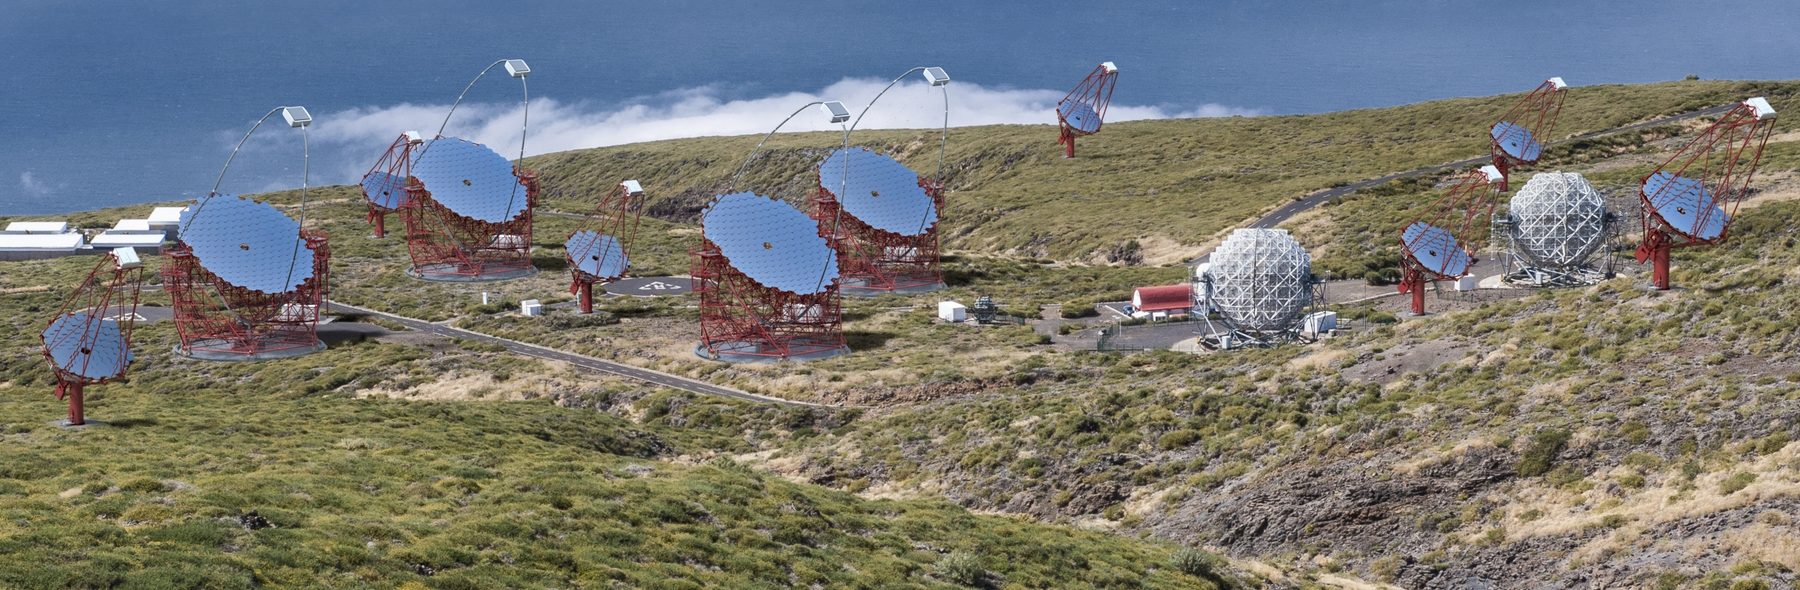
\includegraphics[width=\textwidth]{graphics/cta_north_render.jpg}
      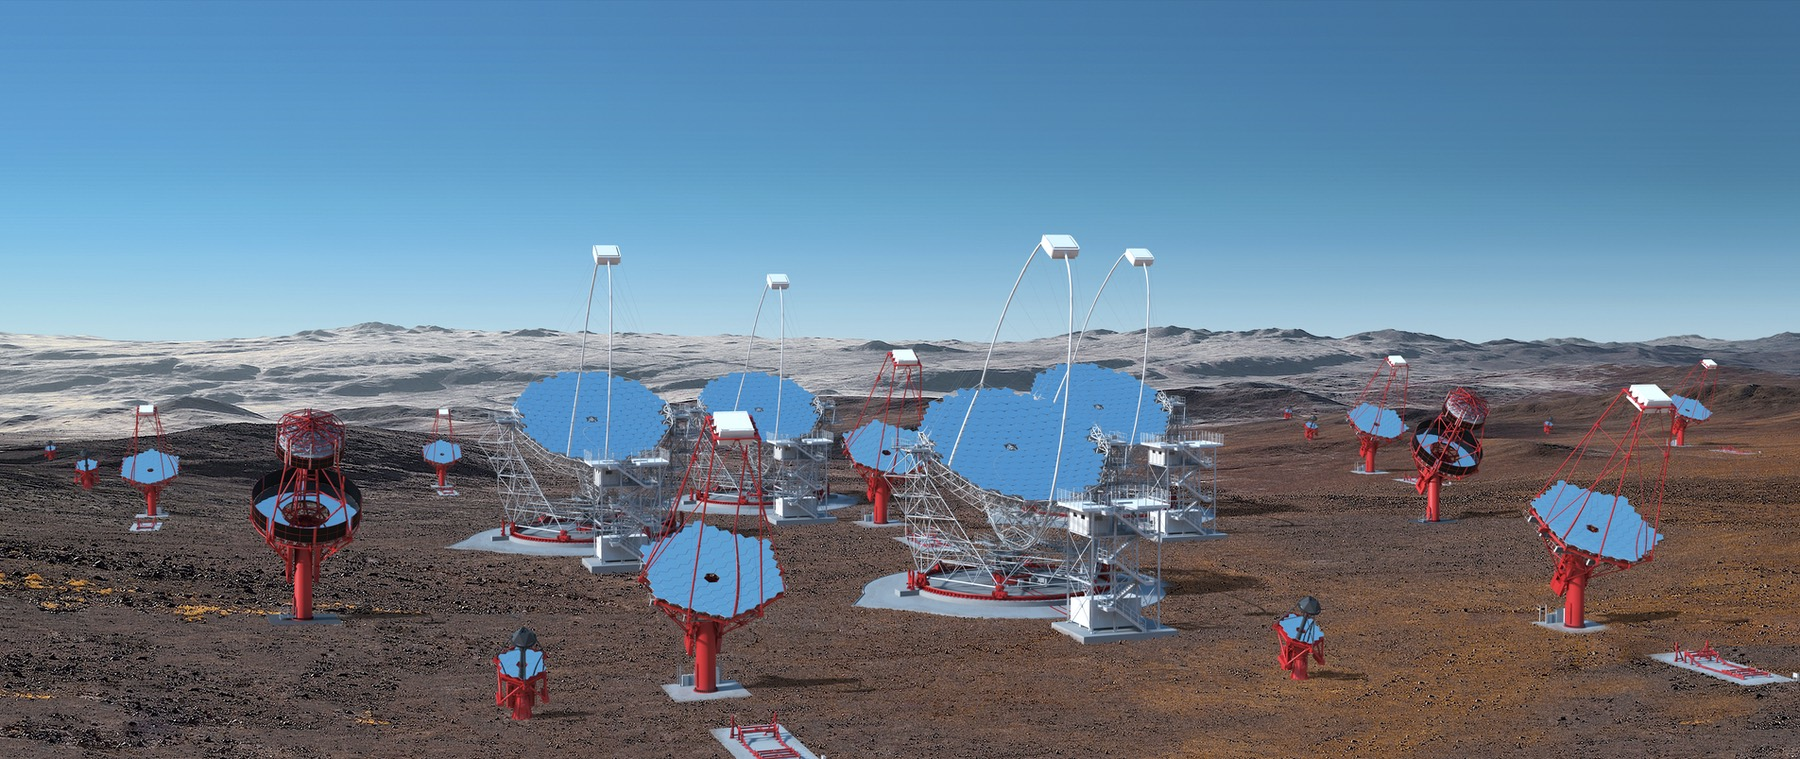
\includegraphics[width=\textwidth]{graphics/cta_south_render.jpg}
      \ifdefined\darktheme
        \footnote{\textcolor{white!85!black}{Image Credit: G.~Pérez Diaz (CTA/IAC)}}
      \else
        \footcite[\textcolor{darkgray!85!black}{Image Credit:}][]{perezdiaz}
      \fi
    \end{center}
  \end{minipage}
\end{frame}


\subsection{CTAs low-level data processing pipeline software: \texttt{ctapipe}}
\begin{frame}{\texttt{ctapipe}}
  \centering
  \ifdefined\darktheme
    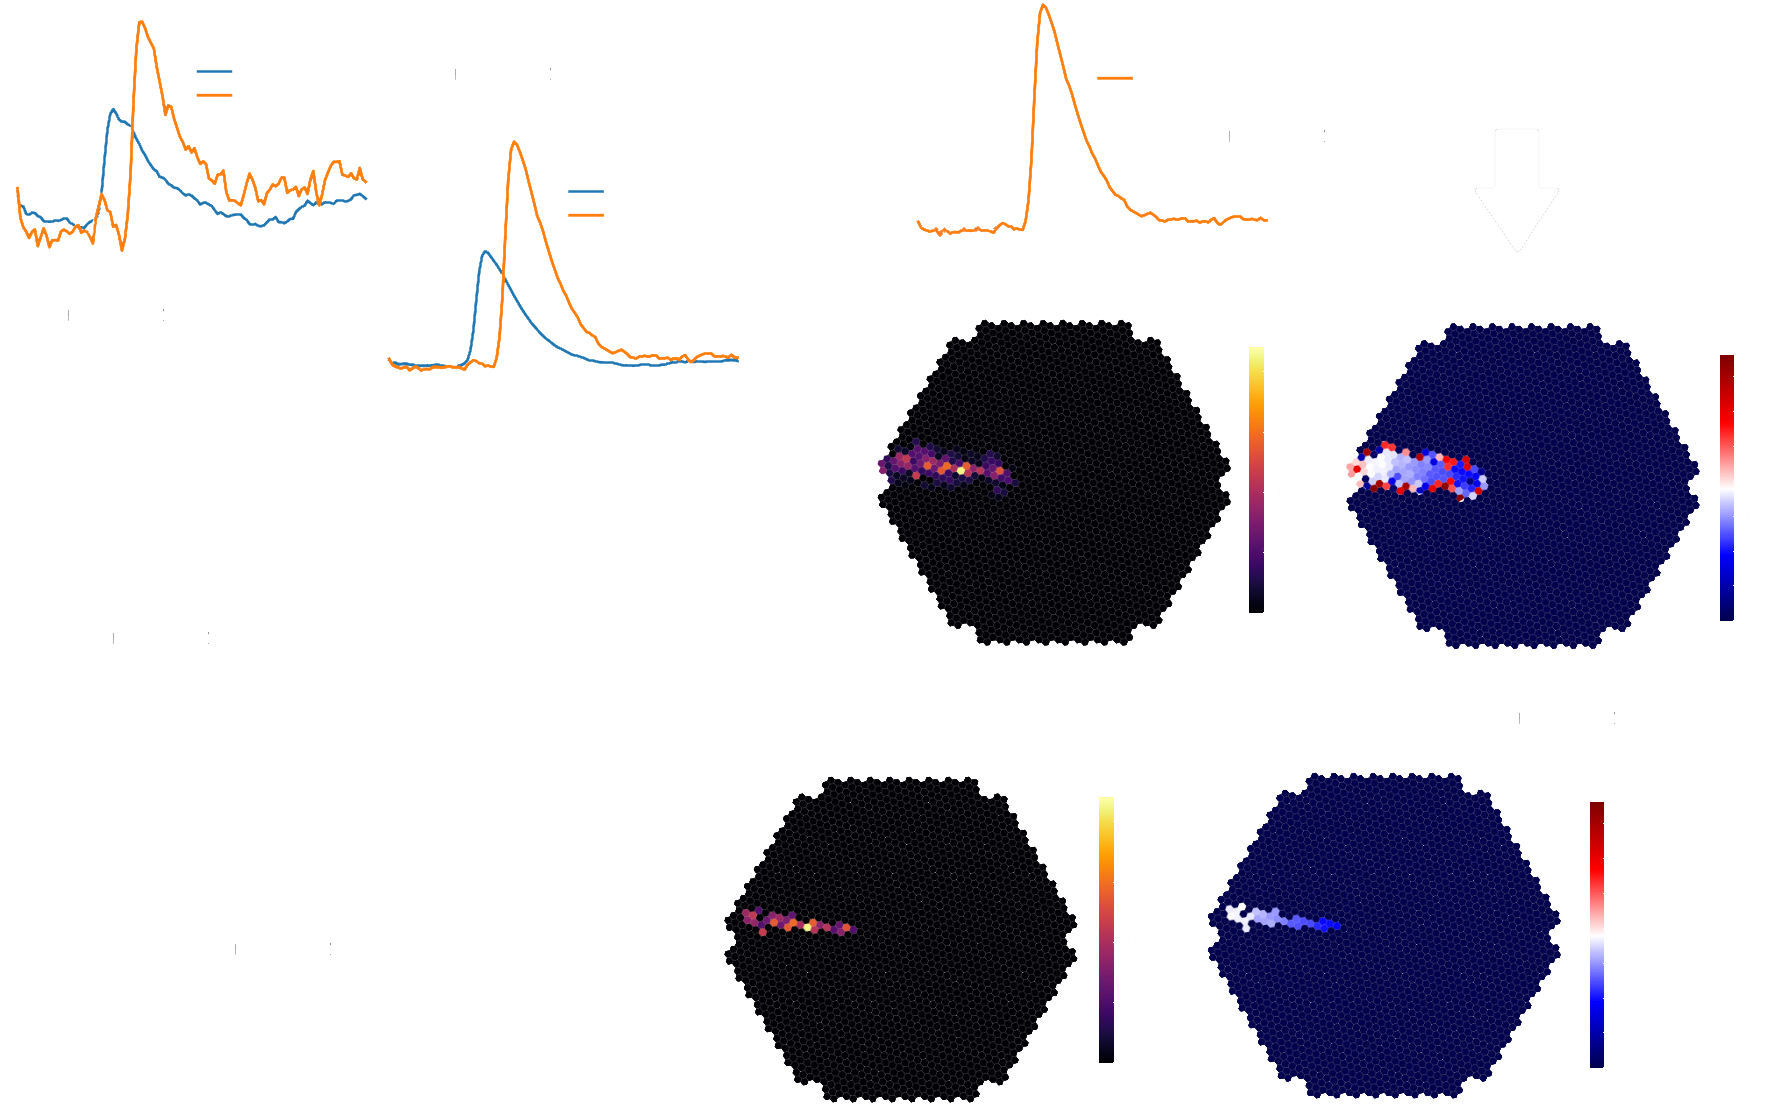
\includegraphics[width=0.7\textwidth]{graphics/ctapipe_darktheme.png}
    \footnote{\textcolor{white!85!black}{Adapted from J.~Hackfeld and M.~Nöthe}}
  \else
    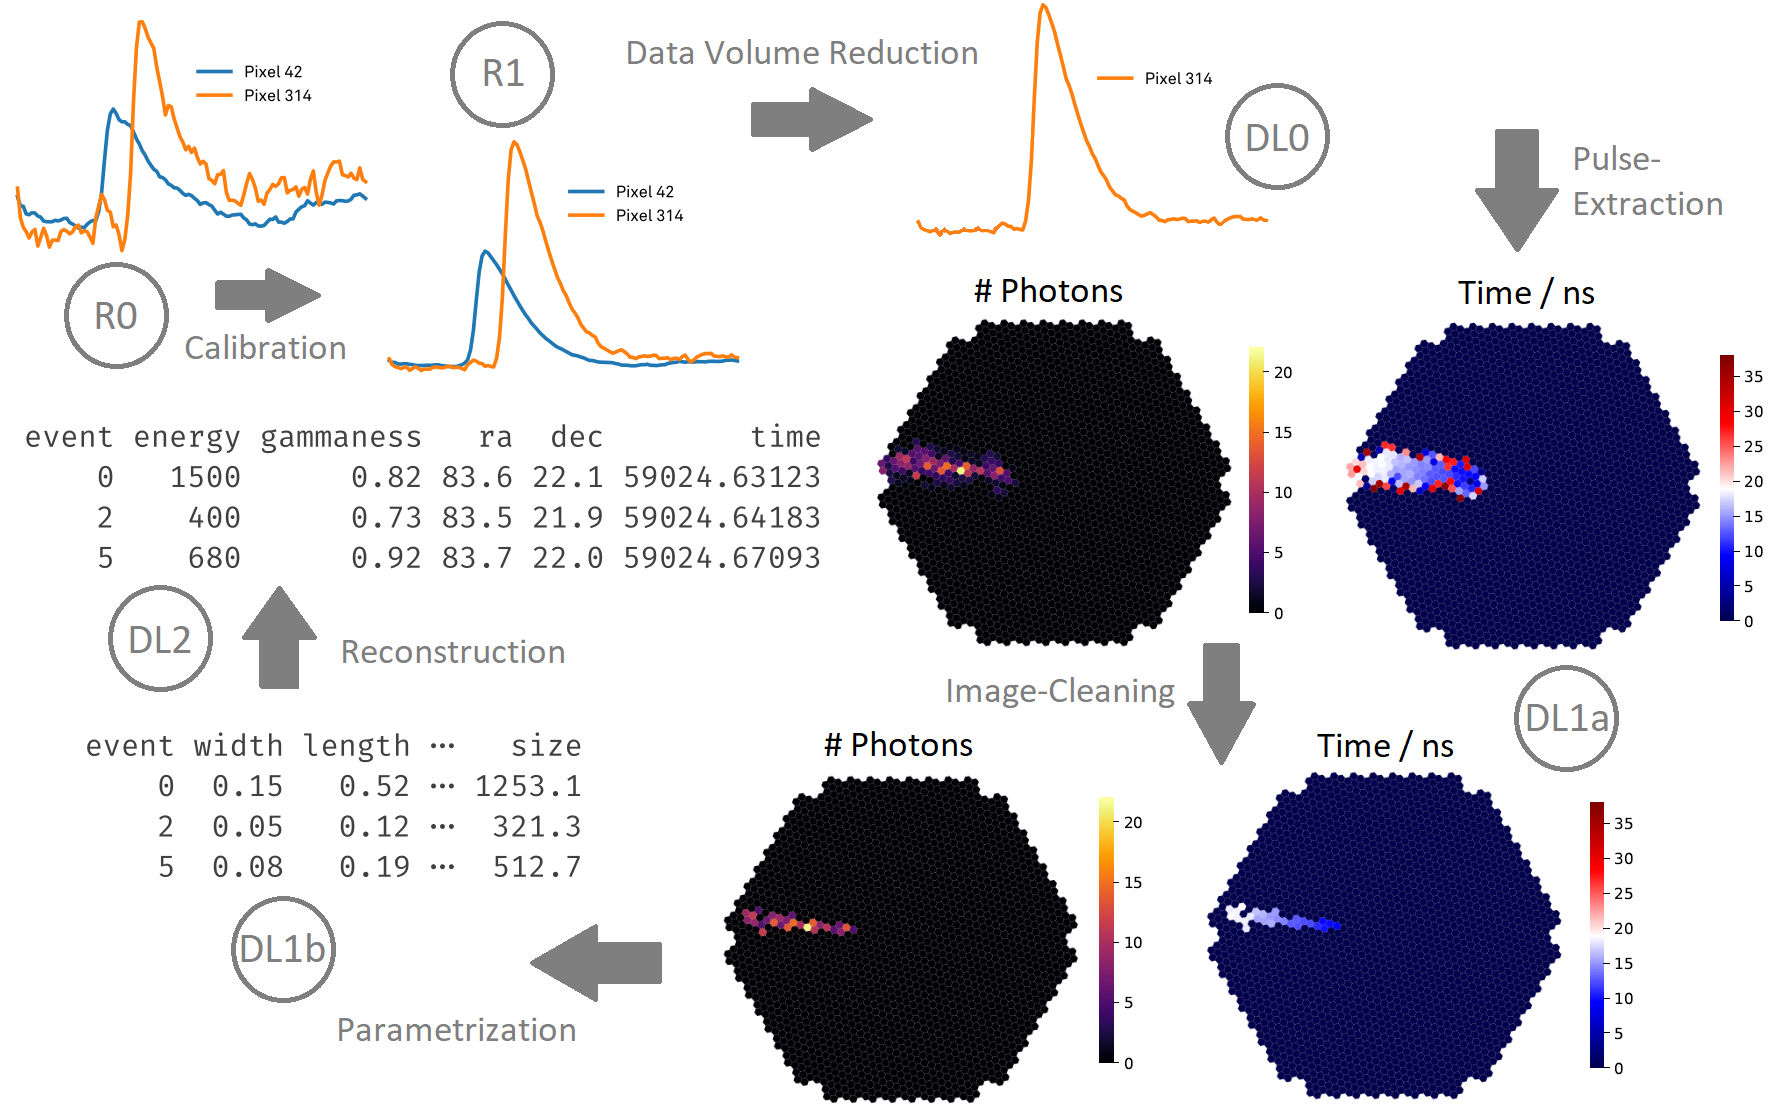
\includegraphics[width=0.7\textwidth]{graphics/ctapipe.png}
    \footcite[\textcolor{darkgray!85!black}{Image Credit:}][]{hackfeld}
  \fi
\end{frame}

\subsection{Cleaning Algorithms}
\ifdefined\darktheme
  \begin{frame}[t]{Cleaning Algorithms}
    \raisebox{10ex}{
    \begin{overlayarea}{0.36\textwidth}{3.5cm}
      \only<1>{
      \begin{itemize}
        \setlength\itemsep{1em}
        \item \code{white}{TailcutsImageCleaner}
        \item \code{white}{MARSImageCleaner}
        \item \code{white}{FACTImageCleaner}
        \item \code{white}{TimeConstrainedImageCleaner}
      \end{itemize}
      }
      \only<2>{
      \begin{itemize}
        \setlength\itemsep{1em}
        \item \code{white}{TailcutsImageCleaner}
        \item \code{white!50!black}{MARSImageCleaner}
        \item \code{white!50!black}{FACTImageCleaner}
        \item \code{white!50!black}{TimeConstrainedImageCleaner}
      \end{itemize}
      }
      \only<3>{
      \begin{itemize}
        \setlength\itemsep{1em}
        \item \code{white!50!black}{TailcutsImageCleaner}
        \item \code{white}{MARSImageCleaner}
        \item \code{white!50!black}{FACTImageCleaner}
        \item \code{white!50!black}{TimeConstrainedImageCleaner}
      \end{itemize}
      }
      \only<4>{
      \begin{itemize}
        \setlength\itemsep{1em}
        \item \code{white!50!black}{TailcutsImageCleaner}
        \item \code{white!50!black}{MARSImageCleaner}
        \item \code{white}{FACTImageCleaner}
        \item \code{white!50!black}{TimeConstrainedImageCleaner}
      \end{itemize}
      }
      \only<5>{
      \begin{itemize}
        \setlength\itemsep{1em}
        \item \code{white!50!black}{TailcutsImageCleaner}
        \item \code{white!50!black}{MARSImageCleaner}
        \item \code{white!50!black}{FACTImageCleaner}
        \item \code{white}{TimeConstrainedImageCleaner}
      \end{itemize}
      }
    \end{overlayarea}
    }
    \raisebox{10ex}{
    \begin{overlayarea}{0.58\textwidth}{3.5cm}
      \only<2>{
      \begin{itemize}%TailcutsImageCleaner
        \item [•] Selects pixels that pass a \code{white!70!black}{picture} and \code{white!70!black}{boundary threshold}
        \item [•] Most basic implementation of the cleaning algorithms
      \end{itemize}
      }
      \only<3>{
      \begin{itemize}%MARSImageCleaner
        \item [•] Selects pixels that pass a \code{white!70!black}{picture} and \code{white!70!black}{boundary threshold}, analogous to \code{white!70!black}{TailcutsImageCleaner}
        \item [•] Also selects pixels that are a neighbor of a neighbor of a core pixel, if they are above the \code{white!70!black}{boundary threshold}
      \end{itemize}
      }
      \only<4>{
      \begin{enumerate}%FACTImageCleaner
        \item Finds all pixels that contain more photons than the \code{white!70!black}{picture threshold}
        \item Removes pixels with less than \(N\) neighbors
        \item Adds remaining neighbors that are above the \code{white!70!black}{boundary threshold}
        \item Removes pixels that have less than \(N\) neighbors, that arrive within a given timeframe
        \item Removes pixels that have less than \(N\) neighbors
        \item Removes pixels that have less than \(N\) neighbors, arriving within a given timeframe
      \end{enumerate}
      }
      \only<5>{
      \begin{enumerate}%TimeConstrainedImageCleaner
        \item Finds all core pixels above the \code{white!70!black}{picture threshold}
        \item Removes pixels with less than \(N\) neighbors
        \item Removes all pixels that arrive within a time limit of the average arrival time
        \item Finds all neighbboring pixels above the \code{white!70!black}{boundary threshold}
        \item Removes all pixels with less than \(N\) neighbors arriving within a given timeframe
      \end{enumerate}
      }
    \end{overlayarea}
    }
    \only<2>{
      \centering
      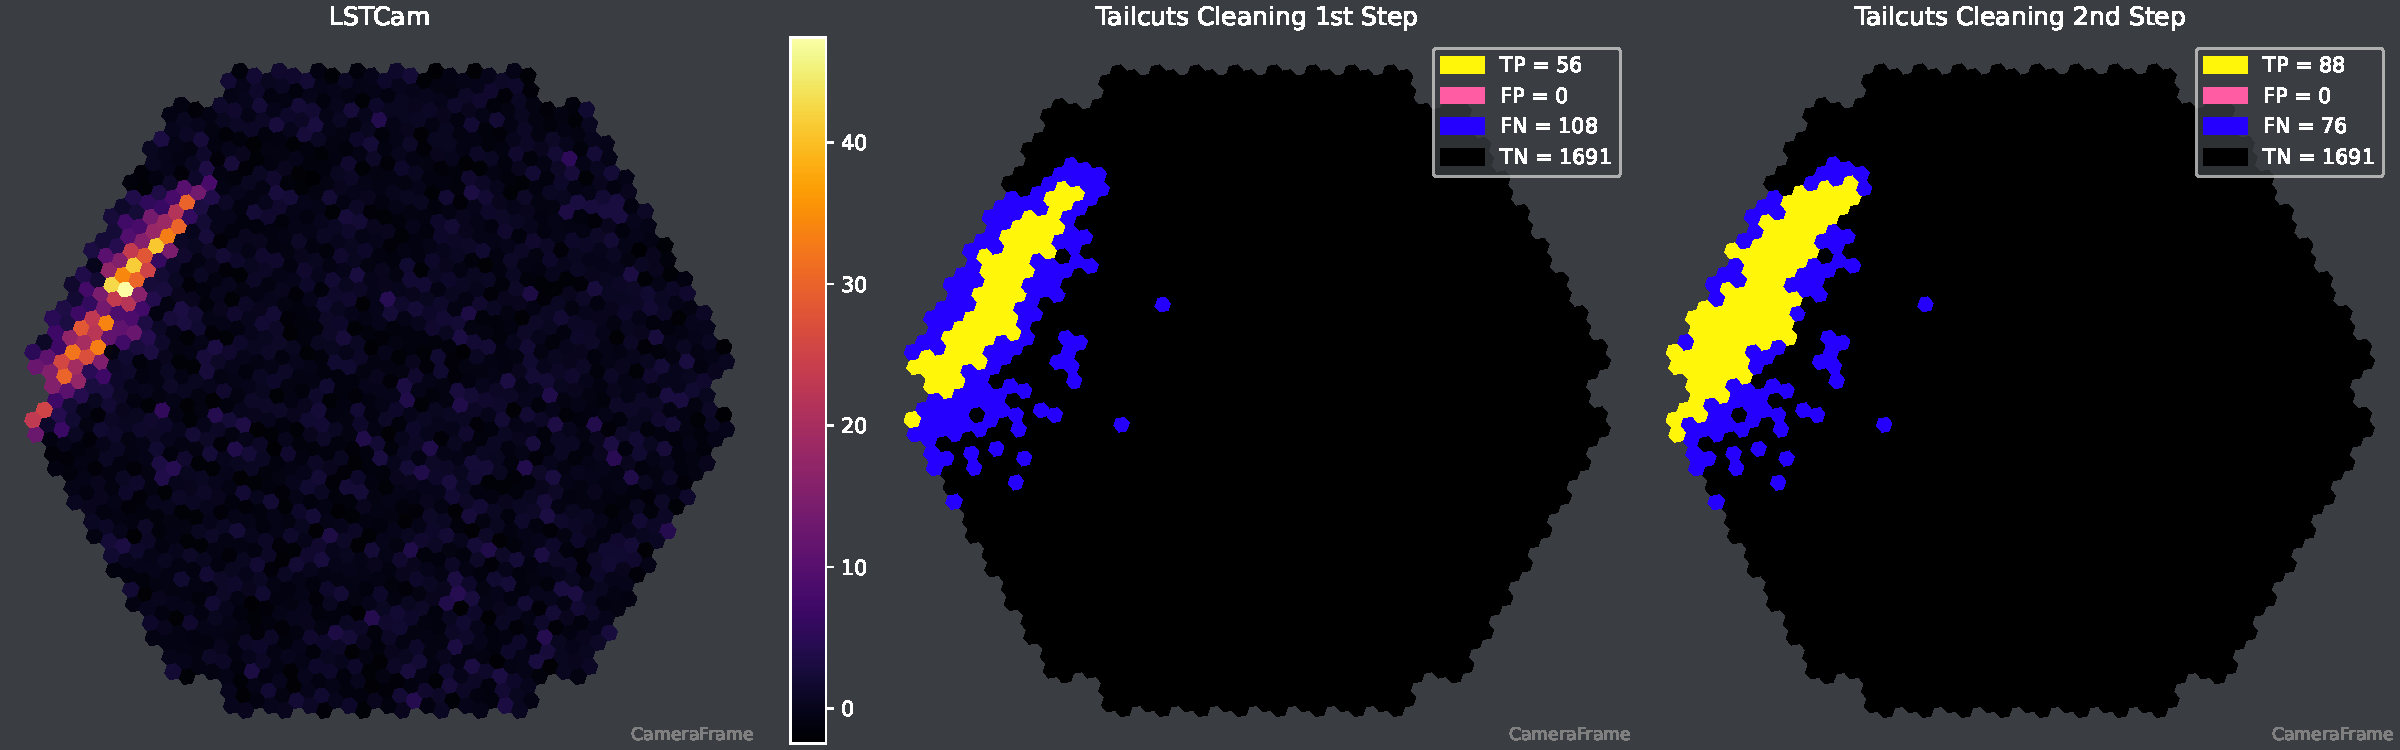
\includegraphics[height=0.15\textwidth]{plots/dl1_plots/run990_999_Tailcuts_event_463.pdf}
    }
    \only<3>{
      \centering
      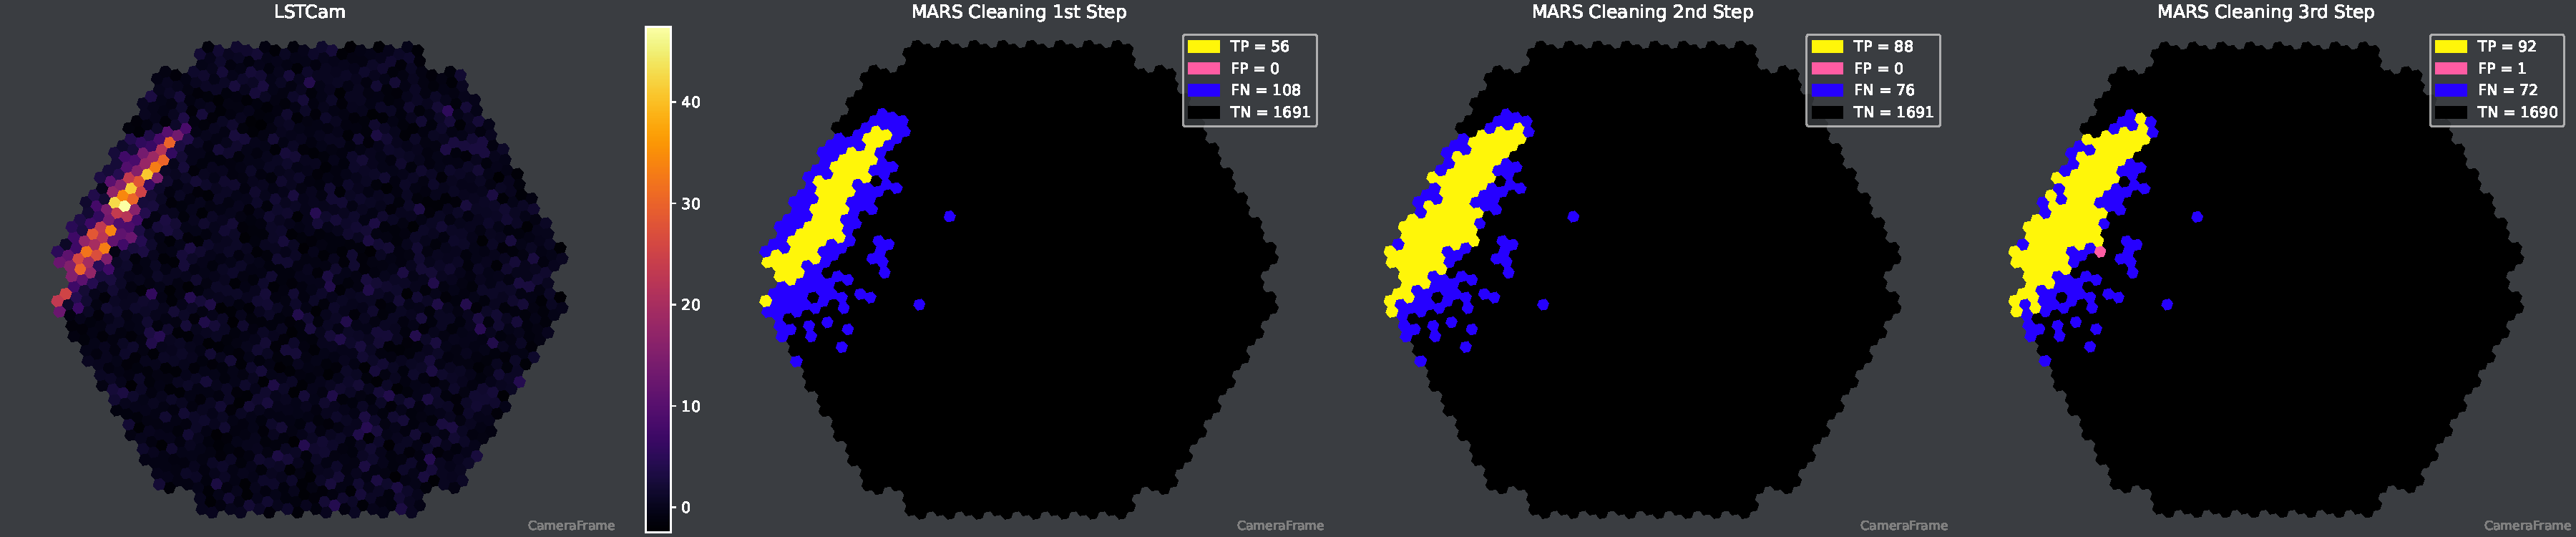
\includegraphics[height=0.15\textwidth]{plots/dl1_plots/run990_999_MARS_event_463.pdf}
    }
    \only<4>{
      \centering
      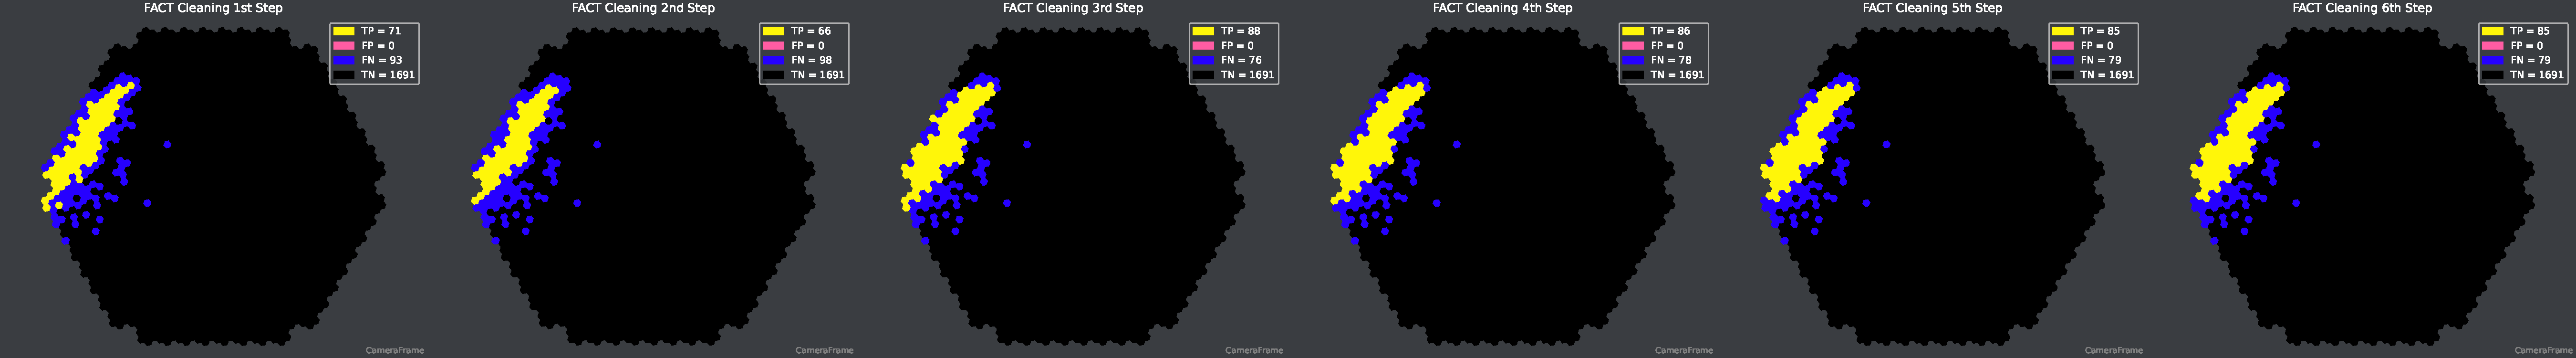
\includegraphics[height=0.13\textwidth]{plots/dl1_plots/run990_999_FACT_event_463.pdf}
    }
    \only<5>{
      \centering
      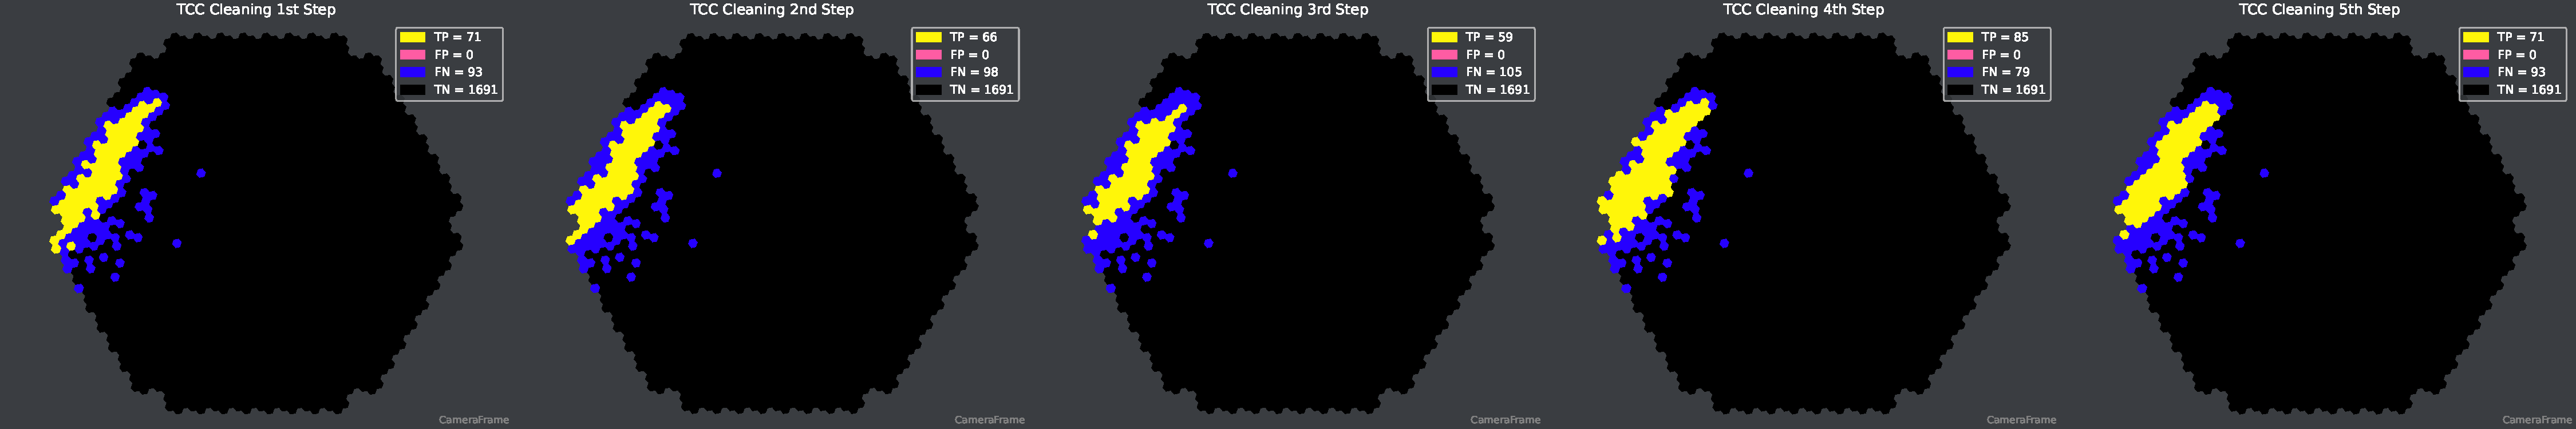
\includegraphics[height=0.15\textwidth]{plots/dl1_plots/run990_999_TCC_event_463.pdf}
    }
  \end{frame}
\else
  \begin{frame}{Cleaning Algorithms}
    \raisebox{10ex}{
    \begin{overlayarea}{0.36\textwidth}{3.5cm}
      \only<1>{
      \begin{itemize}
        \setlength\itemsep{1em}
        \item \code{darkgray}{TailcutsImageCleaner}
        \item \code{darkgray}{MARSImageCleaner}
        \item \code{darkgray}{FACTImageCleaner}
        \item \code{darkgray}{TimeConstrainedImageCleaner}
      \end{itemize}
      }
      \only<2>{
      \begin{itemize}
        \setlength\itemsep{1em}
        \item \code{darkgray}{TailcutsImageCleaner}
        \item \code{lightergray}{MARSImageCleaner}
        \item \code{lightergray}{FACTImageCleaner}
        \item \code{lightergray}{TimeConstrainedImageCleaner}
      \end{itemize}
      }
      \only<3>{
      \begin{itemize}
        \setlength\itemsep{1em}
        \item \code{lightergray}{TailcutsImageCleaner}
        \item \code{darkgray}{MARSImageCleaner}
        \item \code{lightergray}{FACTImageCleaner}
        \item \code{lightergray}{TimeConstrainedImageCleaner}
      \end{itemize}
      }
      \only<4>{
      \begin{itemize}
        \setlength\itemsep{1em}
        \item \code{lightergray}{TailcutsImageCleaner}
        \item \code{lightergray}{MARSImageCleaner}
        \item \code{darkgray}{FACTImageCleaner}
        \item \code{lightergray}{TimeConstrainedImageCleaner}
      \end{itemize}
      }
      \only<5>{
      \begin{itemize}
        \setlength\itemsep{1em}
        \item \code{lightergray}{TailcutsImageCleaner}
        \item \code{lightergray}{MARSImageCleaner}
        \item \code{lightergray}{FACTImageCleaner}
        \item \code{darkgray}{TimeConstrainedImageCleaner}
      \end{itemize}
      }
    \end{overlayarea}
    }
    \raisebox{10ex}{
    \begin{overlayarea}{0.58\textwidth}{3.5cm}
      \only<2>{
      \begin{itemize}%TailcutsImageCleaner
        \item [•] Selects pixels that pass a \code{lightgray}{picture} and \code{lightgray}{boundary threshold}
        \item [•] Most basic implementation of the cleaning algorithms
      \end{itemize}
      }
      \only<3>{
      \begin{itemize}%MARSImageCleaner
        \item [•] Selects pixels that pass a \code{lightgray}{picture} and \code{lightgray}{boundary threshold}, analogous to \code{lightgray}{TailcutsImageCleaner}
        \item [•] Also selects pixels that are a neighbor of a neighbor of a core pixel, if they are above the \code{lightgray}{boundary threshold}
      \end{itemize}
      }
      \only<4>{
      \begin{enumerate}%FACTImageCleaner
        \item Finds all pixels that contain more photons than the \code{lightgray}{picture threshold}
        \item Removes pixels with less than \(N\) neighbors
        \item Adds remaining neighbors that are above the \code{lightgray}{boundary threshold}
        \item Removes pixels that have less than \(N\) neighbors, that arrive within a given timeframe
        \item Removes pixels that have less than \(N\) neighbors
        \item Removes pixels that have less than \(N\) neighbors, arriving within a given timeframe
      \end{enumerate}
      }
      \only<5>{
      \begin{enumerate}%TimeConstrainedImageCleaner
        \item Finds all core pixels above the \code{lightgray}{picture threshold}
        \item Removes pixels with less than \(N\) neighbors
        \item Removes all pixels that arrive within a time limit of the average arrival time
        \item Finds all neighbboring pixels above the \code{lightgray}{boundary threshold}
        \item Removes all pixels with less than \(N\) neighbors arriving within a given timeframe
      \end{enumerate}
      }
    \end{overlayarea}
    }
    \only<2>{
      \centering
      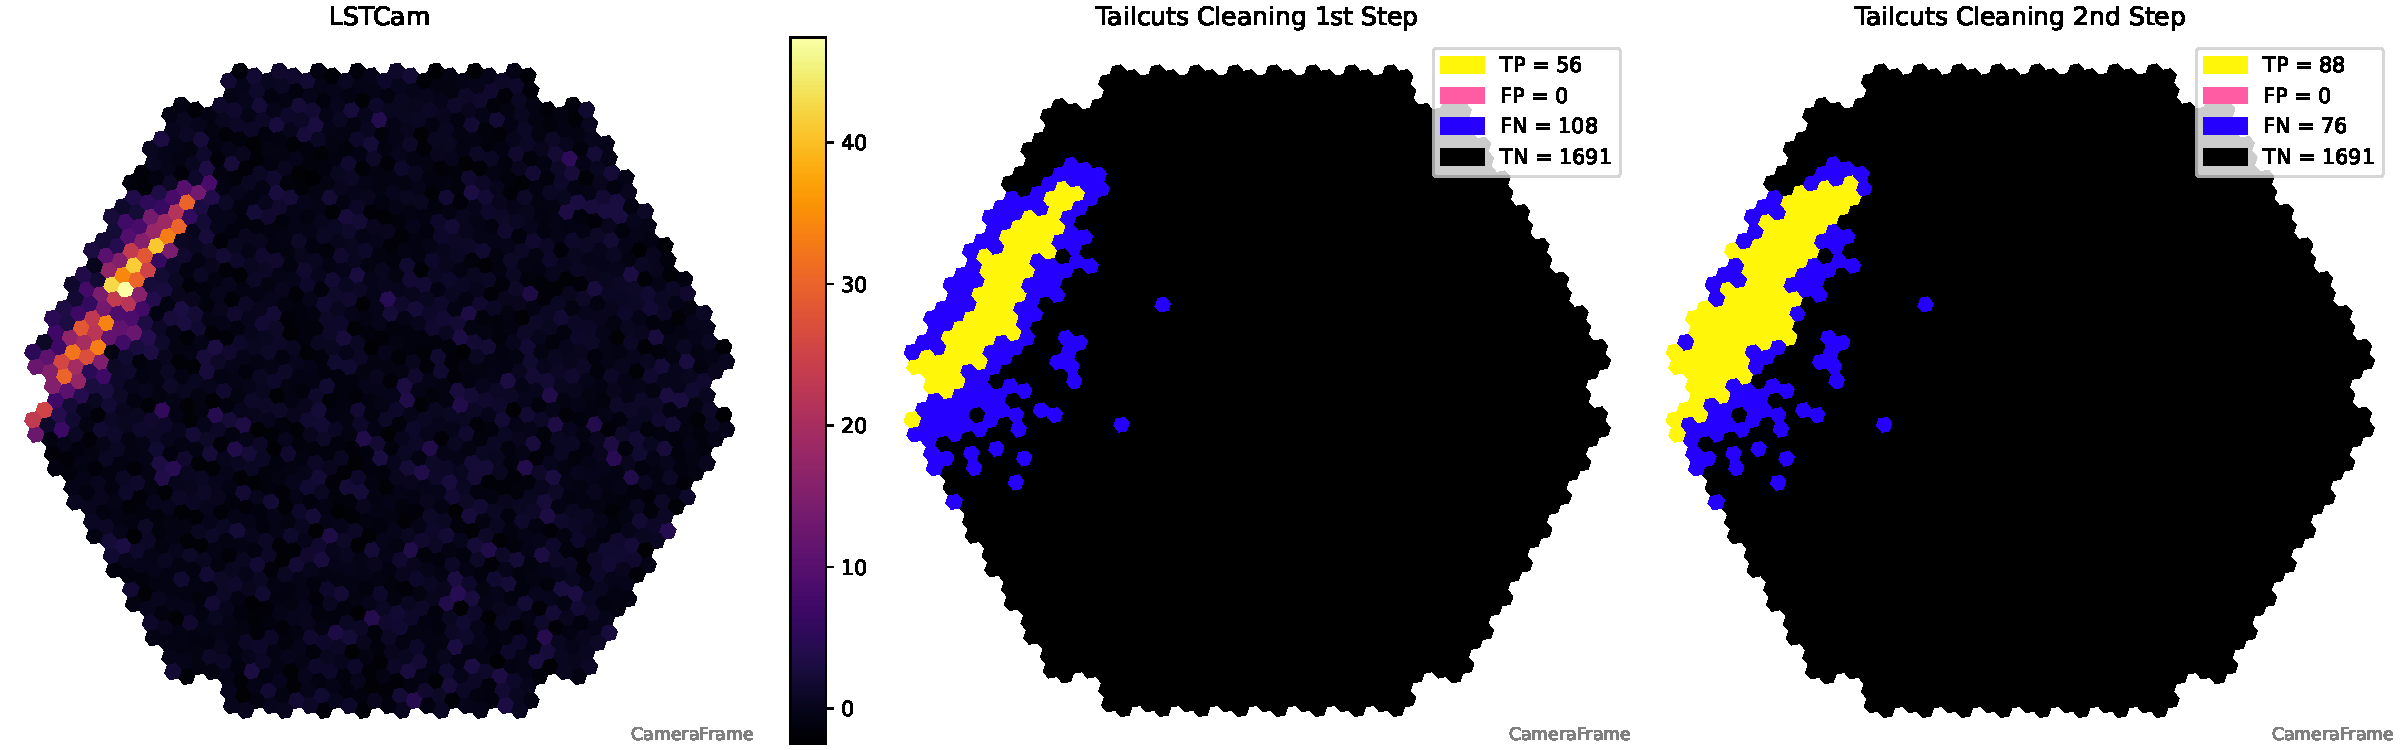
\includegraphics[height=0.15\textwidth]{plots/dl1_plots/run990_999_Tailcuts_event_463_light.pdf}
    }
    \only<3>{
      \centering
      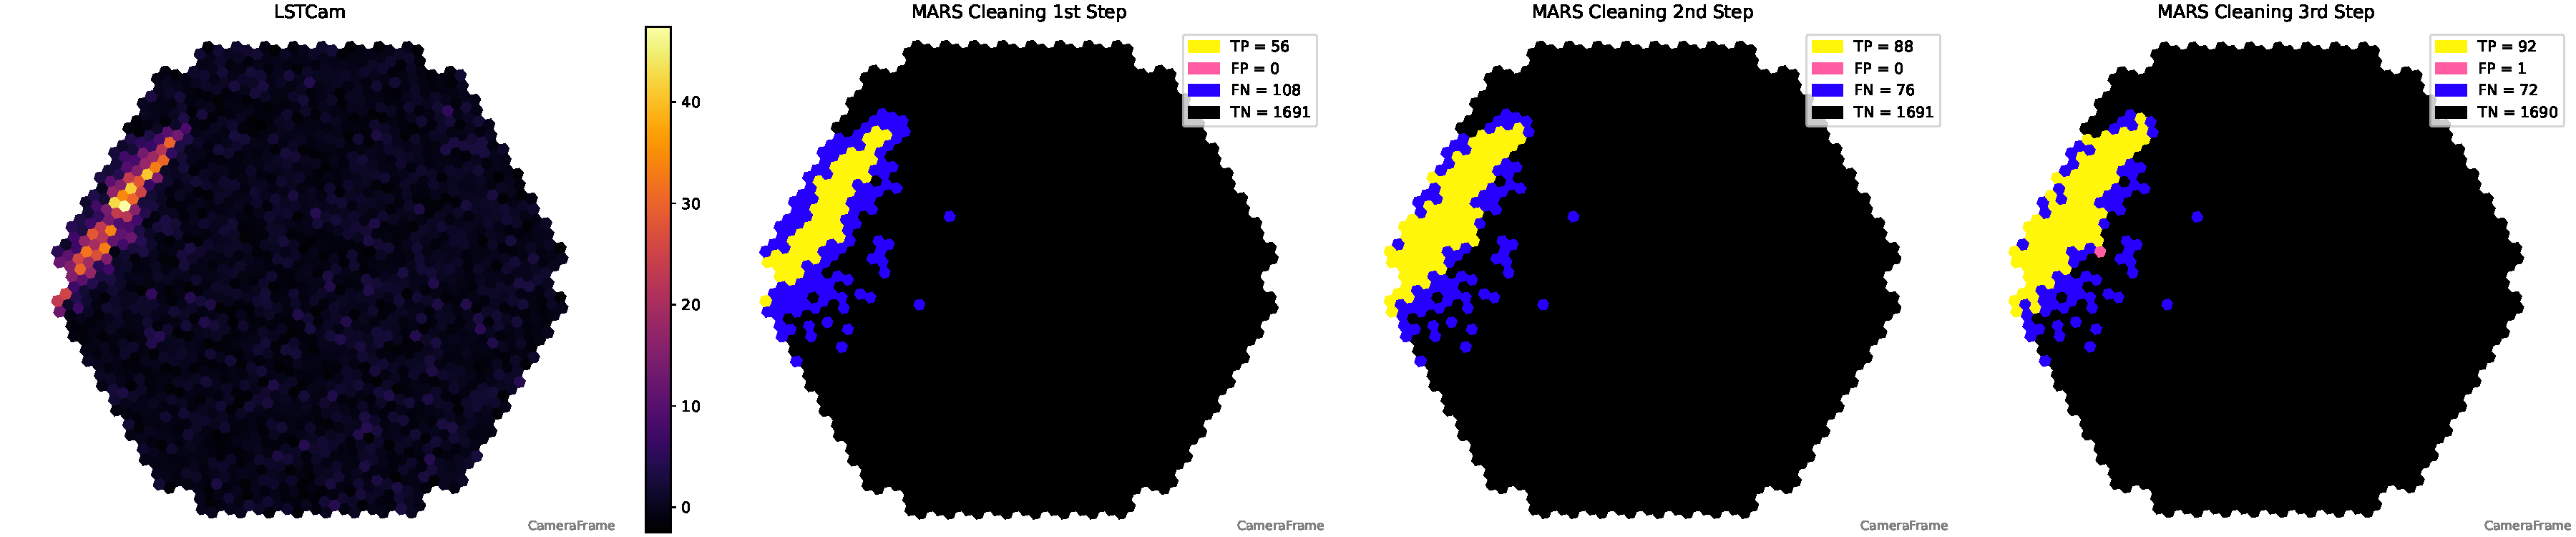
\includegraphics[height=0.15\textwidth]{plots/dl1_plots/run990_999_MARS_event_463_light.pdf}
    }
    \only<4>{
      \centering
      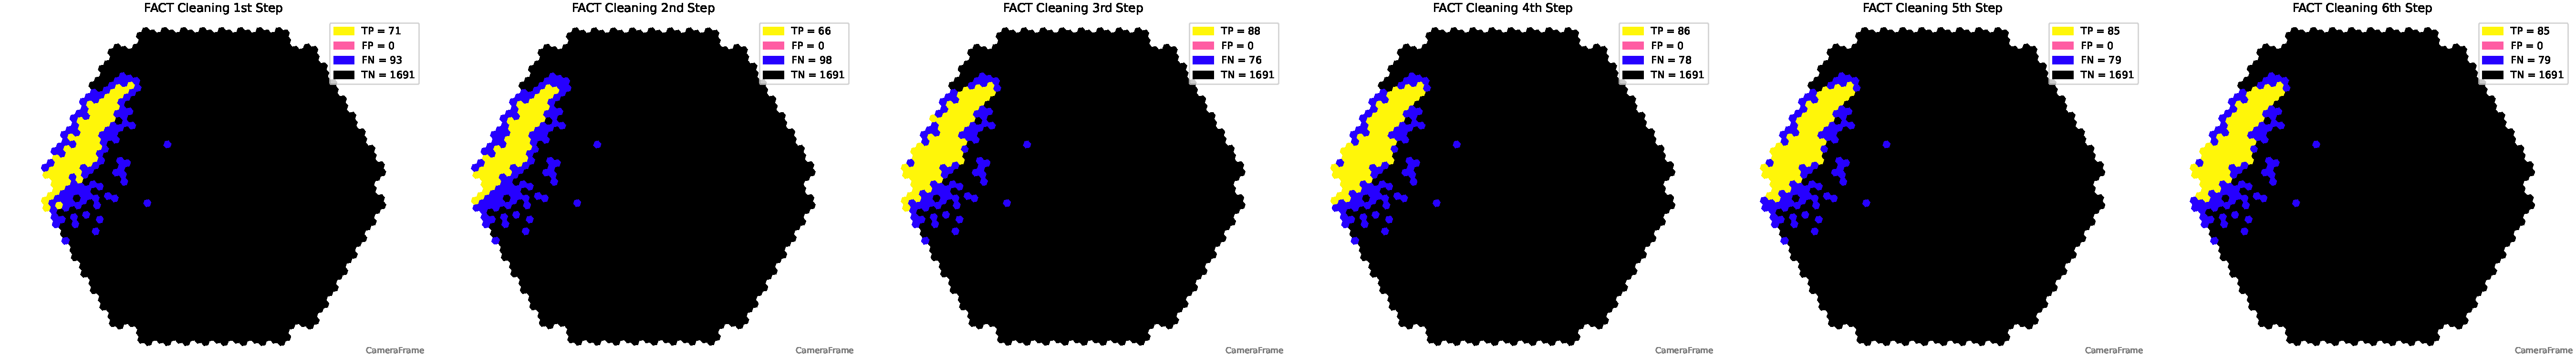
\includegraphics[height=0.13\textwidth]{plots/dl1_plots/run990_999_FACT_event_463_light.pdf}
    }
    \only<5>{
      \centering
      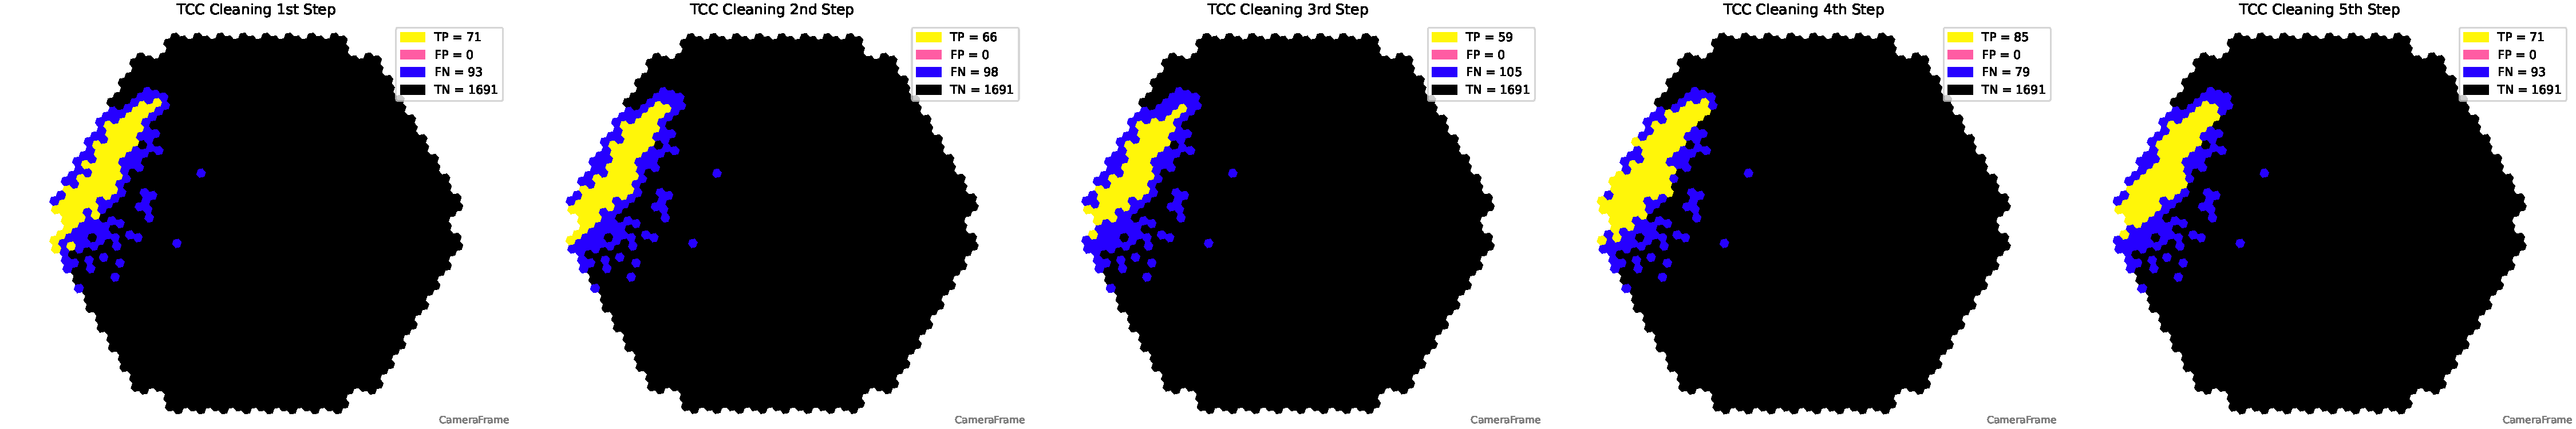
\includegraphics[height=0.15\textwidth]{plots/dl1_plots/run990_999_TCC_event_463_light.pdf}
    }
  \end{frame}
\fi

\section{Data Processing with \texttt{ctapipe}}
\begin{frame}
  \begin{center}
    \textbf{\huge Data Processing with \texttt{ctapipe}}\\
    \begin{tikzpicture}
      \ifdefined\darktheme
        \draw [color=white] (0,0) -- (6,0);
        \draw [color=tugreen] (0,0) -- (2,0);
      \else
        \draw [color=darkgray] (0,0) -- (6,0);
        \draw [color=tugreen] (0,0) -- (2,0);
      \fi
    \end{tikzpicture}
  \end{center}
\end{frame}
\begin{frame}
  \begin{tikzpicture}[scale=0.750, every node/.style={scale=0.8}]
    \node [draw, circle, minimum size=1, align=left] (A) at (0,0) {Simulation Data};

    \uncover<2->{
    \ifdefined\darktheme
        \fill [color=tulightgreen, fill opacity=0.7] (1.5,3) rectangle (7.5, -3);
        \node at (4.5,2) [above] {
\includegraphics[width=2cm]{logos/ctapipe_logo_light.pdf}};
        \node at (4.5,2) {\code{white}{v0.15.1}}; %v0.15.1.dev166+gf26107f
    \else
        \fill [color=tugreen, fill opacity=0.3] (1.5,3) rectangle (7.5, -3);
        \node at (4.5,2) [above] {
\includegraphics[width=2cm]{logos/ctapipe_logo.png}};
        \node at (4.5,2) [below] {\code{darkgray}{v0.15.1}};
    \fi
    \node [draw, circle, minimum size=1] (B) at (3,0) {\texttt{ctapipe-process}};
    \draw [->, >=latex, to path={-- (\tikztotarget)}] (A) edge (B);
    }

    \uncover<3->{
    \node [above] at (4.5,-2) {Run with python scripts and configs};
    \node [draw, align=left] (BC) at (4.5,-2.5) {\texttt{cleaner\_config.yml}\\\texttt{prod5b\_lapalma\_alpha.yml}};
    }

    \only<3>{
        \ifdefined\darktheme
            \node [draw, color=darkmode, align=left] at (13.5,-0.11) {
                \code{yamlblue}{ImageProcessor}\code{white}{:}\\
                \bigskip
                \quad\code{yamlblue}{image_cleaner_type}\code{white}{:} \code{yamlblue}{MARSImageCleaner}\\
                \quad\quad\code{yamlblue}{MARSImageCleaner}\code{white}{:}\\
                \quad\quad\quad\code{yamlblue}{picture_threshold_pe}\code{white}{:}\\
                \quad\quad\quad\quad\code{white}{-} \code{yamlyellow}{[}\code{white}{type,} \code{yamlorange}{"LST*"}\code{white}{, 8.5}\code{yamlyellow}{]}\\
                \quad\quad\quad\quad\code{white}{-} \code{yamlyellow}{[}\code{white}{type,} \code{yamlorange}{"MST*NectarCam"}\code{white}{, 9.0}\code{yamlyellow}{]}\\
                \quad\quad\quad\code{yamlblue}{boundary_threshold_pe}\code{white}{:}\\
                \quad\quad\quad\quad\code{white}{-} \code{yamlyellow}{[}\code{white}{type,} \code{yamlorange}{"LST*"}\code{white}{, 4.75}\code{yamlyellow}{]}\\
                \quad\quad\quad\quad\code{white}{-} \code{yamlyellow}{[}\code{white}{type,} \code{yamlorange}{"MST*NectarCam"}\code{white}{, 4.5}\code{yamlyellow}{]}\\
                \quad\quad\quad\code{yamlblue}{keep_isolated_pixels}\code{white}{:} \code{yamlblue}{false}\\
                \bigskip
                \quad\quad\quad\code{yamlblue}{min_picture_neighbors}\code{white}{: 2}\\
                \quad\quad\code{yamlblue}{ImageQualityQuery}\code{white}{:}\\
                \quad\quad\quad\code{yamlblue}{quality_criteria}\code{white}{:}\\
                \quad\quad\quad\quad\code{white}{-} \code{yamlyellow}{[}\code{yamlorange}{"enough_pixels"}\code{white}{,} \code{yamlorange}{"np.count_nonzero(image) > 2"}\code{yamlyellow}{]}\\
                \quad\quad\quad\quad\code{white}{-} \code{yamlyellow}{[}\code{yamlorange}{"enough_charge"}\code{white}{,} \code{yamlorange}{"image.sum() > 50"}\code{yamlyellow}{]}
            };
        \else
            \node [draw, color=white, align=left] at (13.5,-0.11) {
                \code{yamlblue}{ImageProcessor}\code{darkgray}{:}\\
                \bigskip
                \quad\code{yamlblue}{image_cleaner_type}\code{darkgray}{:} \code{yamlblue}{MARSImageCleaner}\\
                \quad\quad\code{yamlblue}{MARSImageCleaner}\code{darkgray}{:}\\
                \quad\quad\quad\code{yamlblue}{picture_threshold_pe}\code{darkgray}{:}\\
                \quad\quad\quad\quad\code{darkgray}{-} \code{yamlyellow}{[}\code{darkgray}{type,} \code{yamlorange}{"LST*"}\code{darkgray}{, 8.5}\code{yamlyellow}{]}\\
                \quad\quad\quad\quad\code{darkgray}{-} \code{yamlyellow}{[}\code{darkgray}{type,} \code{yamlorange}{"MST*NectarCam"}\code{darkgray}{, 9.0}\code{yamlyellow}{]}\\
                \quad\quad\quad\code{yamlblue}{boundary_threshold_pe}\code{darkgray}{:}\\
                \quad\quad\quad\quad\code{darkgray}{-} \code{yamlyellow}{[}\code{darkgray}{type,} \code{yamlorange}{"LST*"}\code{darkgray}{, 4.75}\code{yamlyellow}{]}\\
                \quad\quad\quad\quad\code{darkgray}{-} \code{yamlyellow}{[}\code{darkgray}{type,} \code{yamlorange}{"MST*NectarCam"}\code{darkgray}{, 4.5}\code{yamlyellow}{]}\\
                \quad\quad\quad\code{yamlblue}{keep_isolated_pixels}\code{darkgray}{:} \code{yamlblue}{false}\\
                \bigskip
                \quad\quad\quad\code{yamlblue}{min_picture_neighbors}\code{darkgray}{: 2}\\
                \quad\quad\code{yamlblue}{ImageQualityQuery}\code{darkgray}{:}\\
                \quad\quad\quad\code{yamlblue}{quality_criteria}\code{darkgray}{:}\\
                \quad\quad\quad\quad\code{darkgray}{-} \code{yamlyellow}{[}\code{yamlorange}{"enough_pixels"}\code{darkgray}{,} \code{yamlorange}{"np.count_nonzero(image) > 2"}\code{yamlyellow}{]}\\
                \quad\quad\quad\quad\code{darkgray}{-} \code{yamlyellow}{[}\code{yamlorange}{"enough_charge"}\code{darkgray}{,} \code{yamlorange}{"image.sum() > 50"}\code{yamlyellow}{]}
            };
        \fi
        \draw [to path={-| (\tikztotarget)}] (BC) to (7.8,0);
        \draw [->, >=latex, to path={-- (\tikztotarget)}] (7.8,0) to (9,0);
    }

    \uncover<4->{
    \node [draw, circle, minimum size=1] (C) at (6,0) {\texttt{ctapipe-merge}};
    \draw [->, >=latex, to path={-- (\tikztotarget)}] (B) edge (C);
    }

    \uncover<5->{
    \fill [color=tublue, fill opacity=0.3] (7.7,3) rectangle (19, -3);
    \node [draw, circle, minimum size=1, align=center] (D) at (9,0) {Processing\\of\\Telescope-\\Level Data};
    \draw [->, >=latex, to path={-- (\tikztotarget)}] (C) edge (D);
    }

    \uncover<6->{
    \node [draw, circle, minimum size=1] (E1) at (12,2) {dl1 plots};
    \node [draw, circle, minimum size=1, align=center] (E2) at (12,0) {Angular\\Resolution\\\&\\Separation};
    \node [draw, circle, minimum size=1] (E3) at (12,-2) {Metrics};

    \draw [->, >=latex, to path={|- (\tikztotarget)}] (D) edge (E1);
    \draw [->, >=latex, to path={-- (\tikztotarget)}] (D) edge (E2);
    \draw [->, >=latex, to path={|- (\tikztotarget)}] (D) edge (E3);
    }

    \uncover<7->{
    \node [draw, circle, minimum size=1, align=center] (F) at (15,0) {Effective\\Area};
    \draw [->, >=latex, to path={-- (\tikztotarget)}] (E2) edge (F);
    }

    \uncover<8->{
    \node [draw, circle, minimum size=1, align=center] (G) at (18,0) {Results/\\Plots};
    \draw [->, >=latex, to path={-- (\tikztotarget)}] (F) edge (G);

    \coordinate (FG) at (16.5,0) {};
    \draw [to path={-| (\tikztotarget)}] (E1) to (FG);
    \draw [to path={-| (\tikztotarget)}] (E3) to (FG);
    }
\end{tikzpicture}
\end{frame}

\section{Results}
\begin{frame}
  \begin{center}
    \textbf{\huge Results}\\
    \begin{tikzpicture}
      \ifdefined\darktheme
        \draw [color=white] (0,0) -- (6,0);
        \draw [color=tugreen] (0,0) -- (4,0);
      \else
        \draw [color=darkgray] (0,0) -- (6,0);
        \draw [color=tugreen] (0,0) -- (4,0);
      \fi
    \end{tikzpicture}
  \end{center}
\end{frame}
\begin{frame}{Angular Separation}
  \begin{minipage}{0.32\textwidth}
    \ifdefined\darktheme
      \centering
      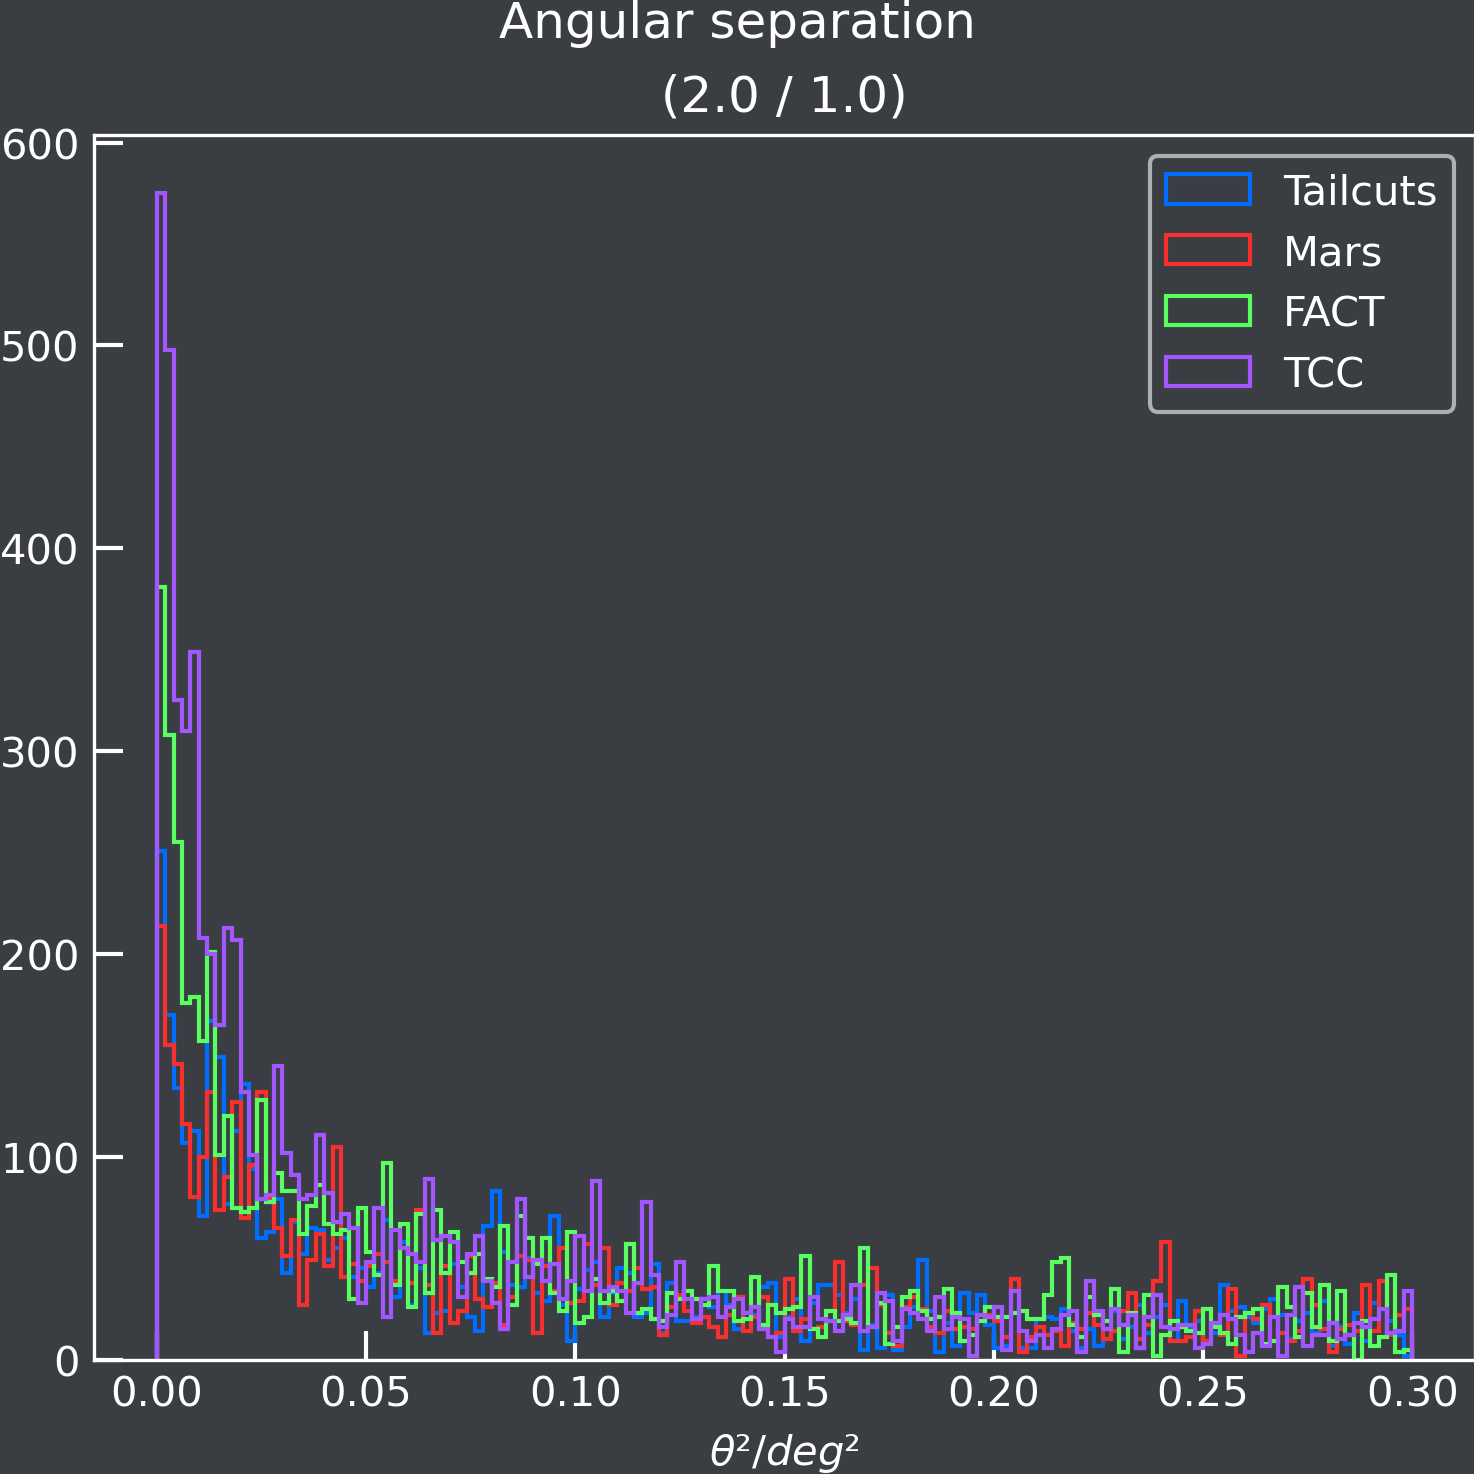
\includegraphics[width=\textwidth]{plots/ang_sep/ang_sep__2.0_1.0_dark.png}
    \else
      \centering
      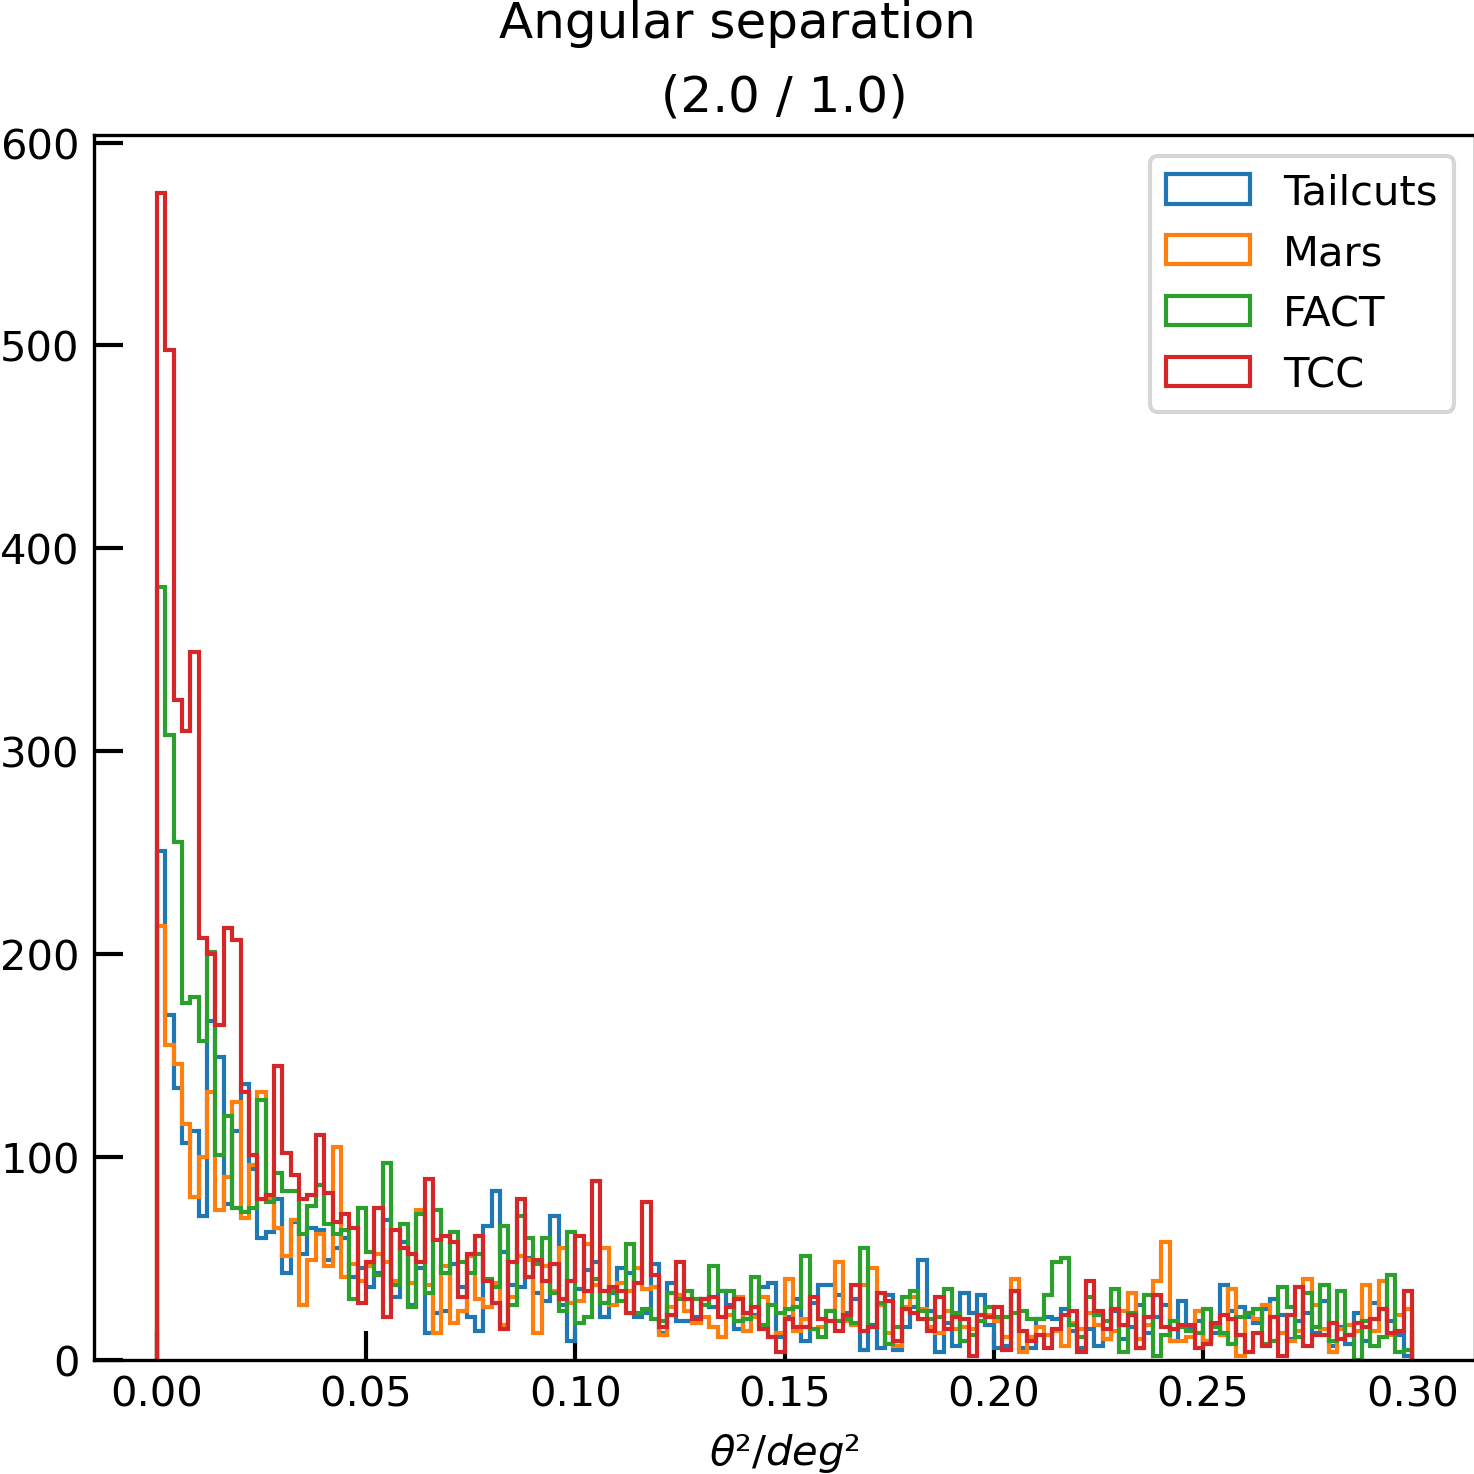
\includegraphics[width=\textwidth]{plots/ang_sep/ang_sep__2.0_1.0_light.png}
    \fi
  \end{minipage}
  \begin{minipage}{0.32\textwidth}
    \ifdefined\darktheme
      \centering
      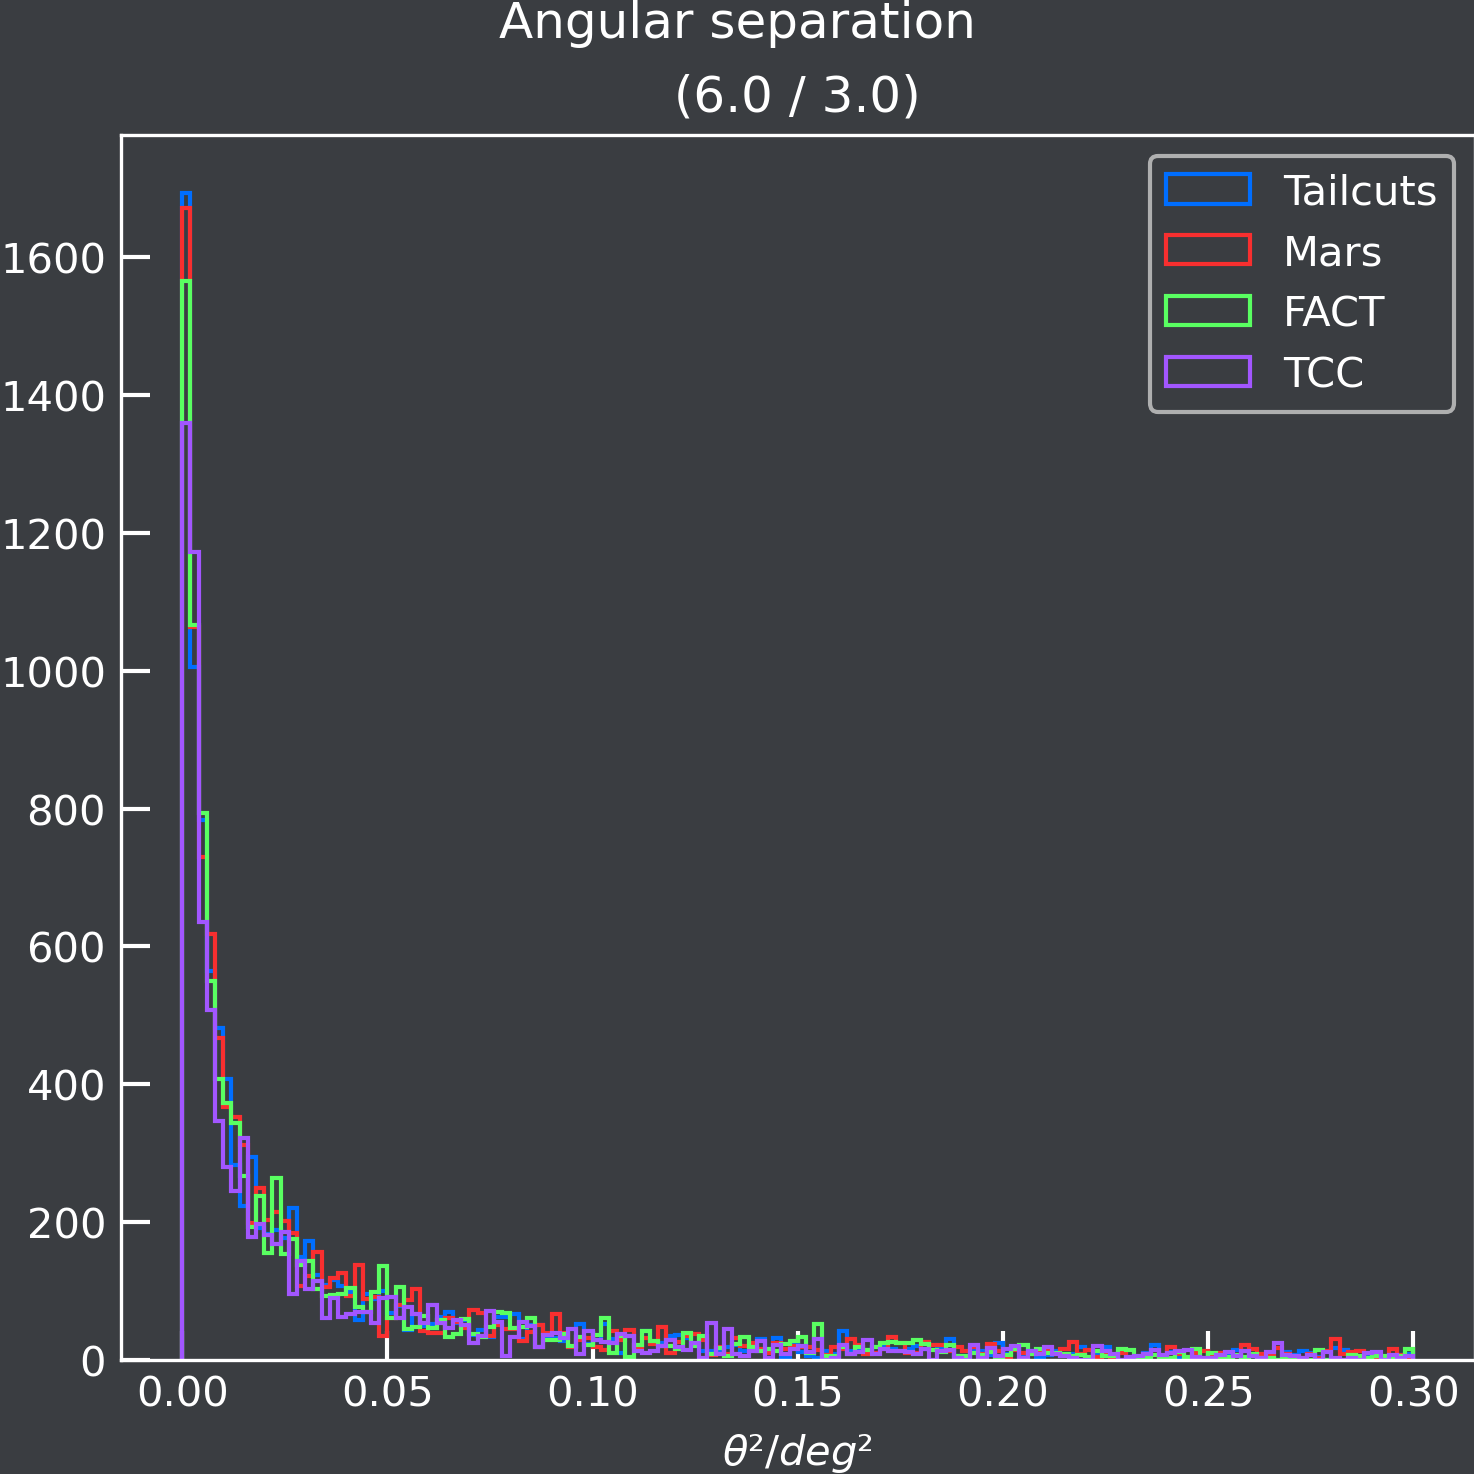
\includegraphics[width=\textwidth]{plots/ang_sep/ang_sep__6.0_3.0_dark.png}
    \else
      \centering
      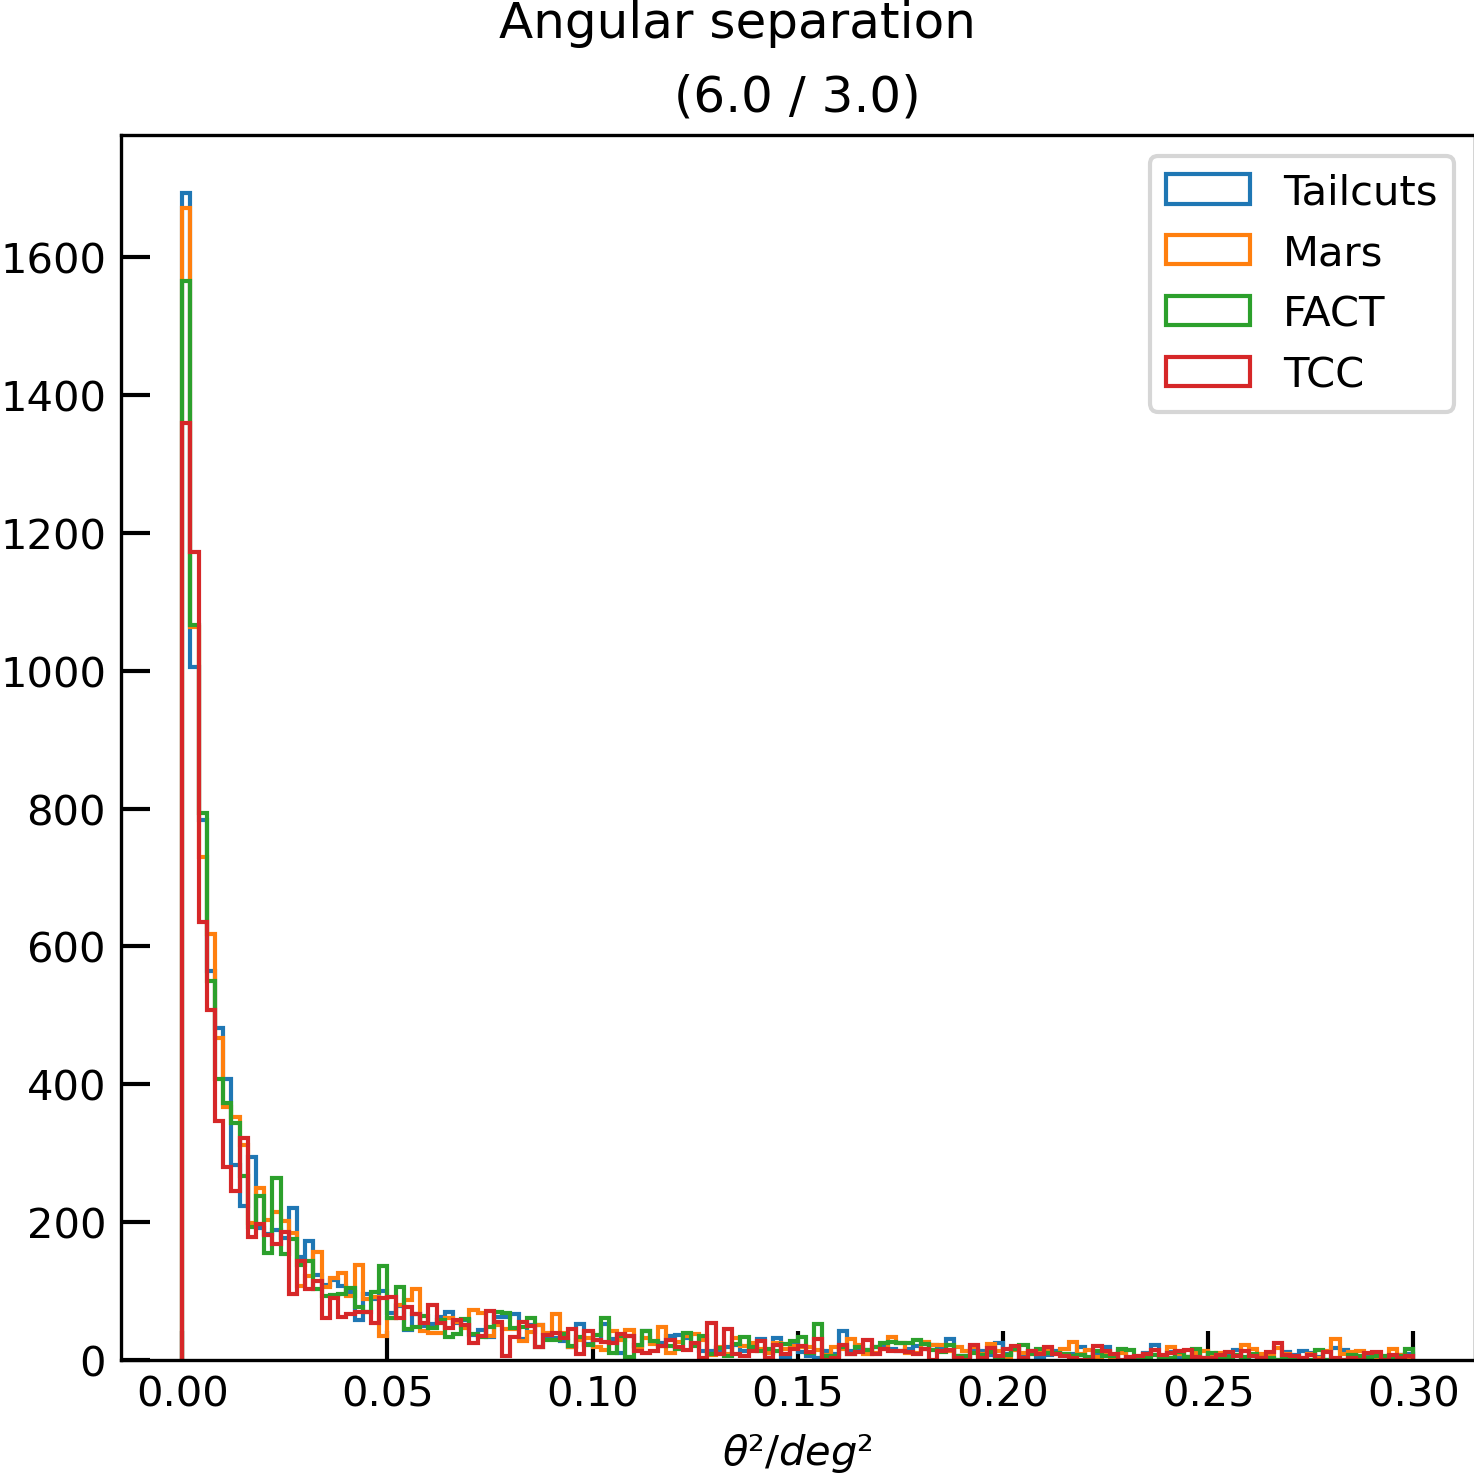
\includegraphics[width=\textwidth]{plots/ang_sep/ang_sep__6.0_3.0_light.png}
    \fi
  \end{minipage}
  \begin{minipage}{0.32\textwidth}
    \ifdefined\darktheme
      \centering
      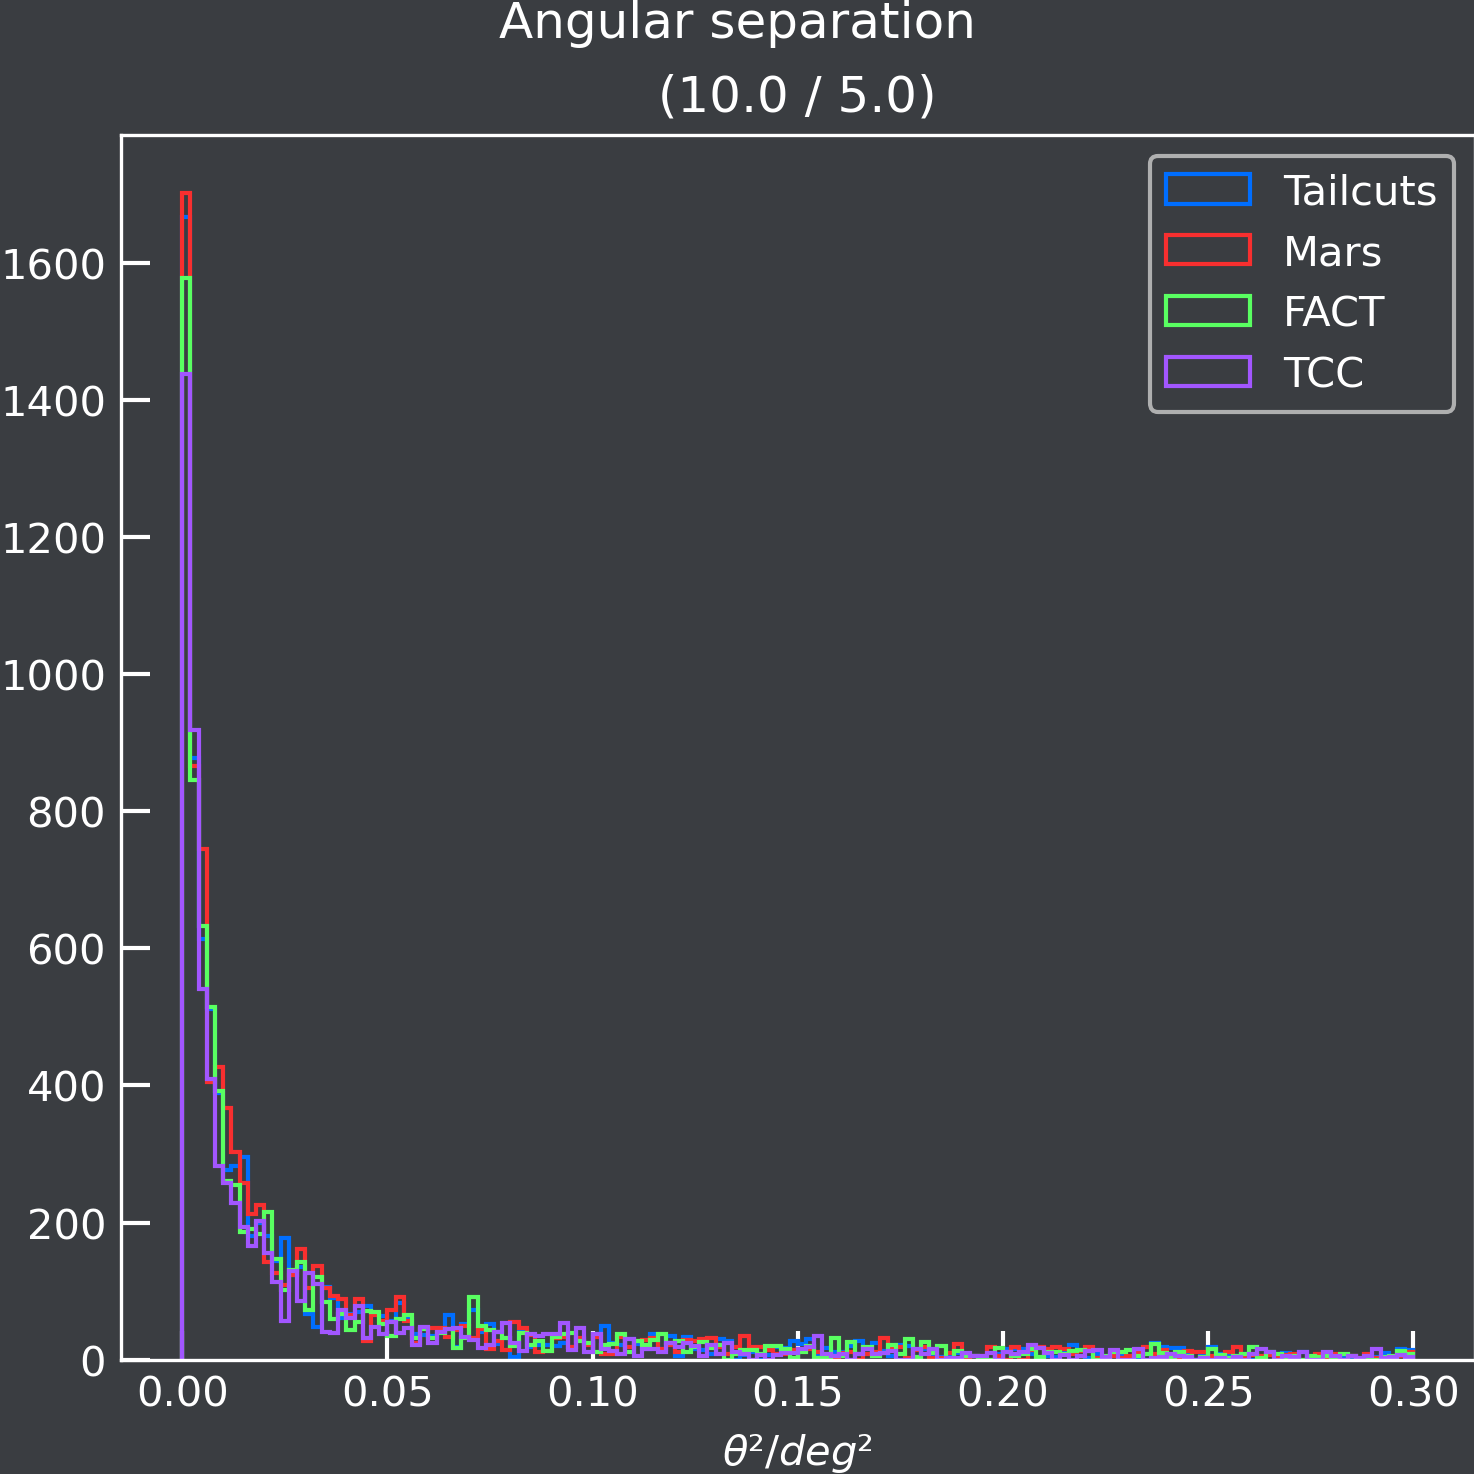
\includegraphics[width=\textwidth]{plots/ang_sep/ang_sep__10.0_5.0_dark.png}
    \else
      \centering
      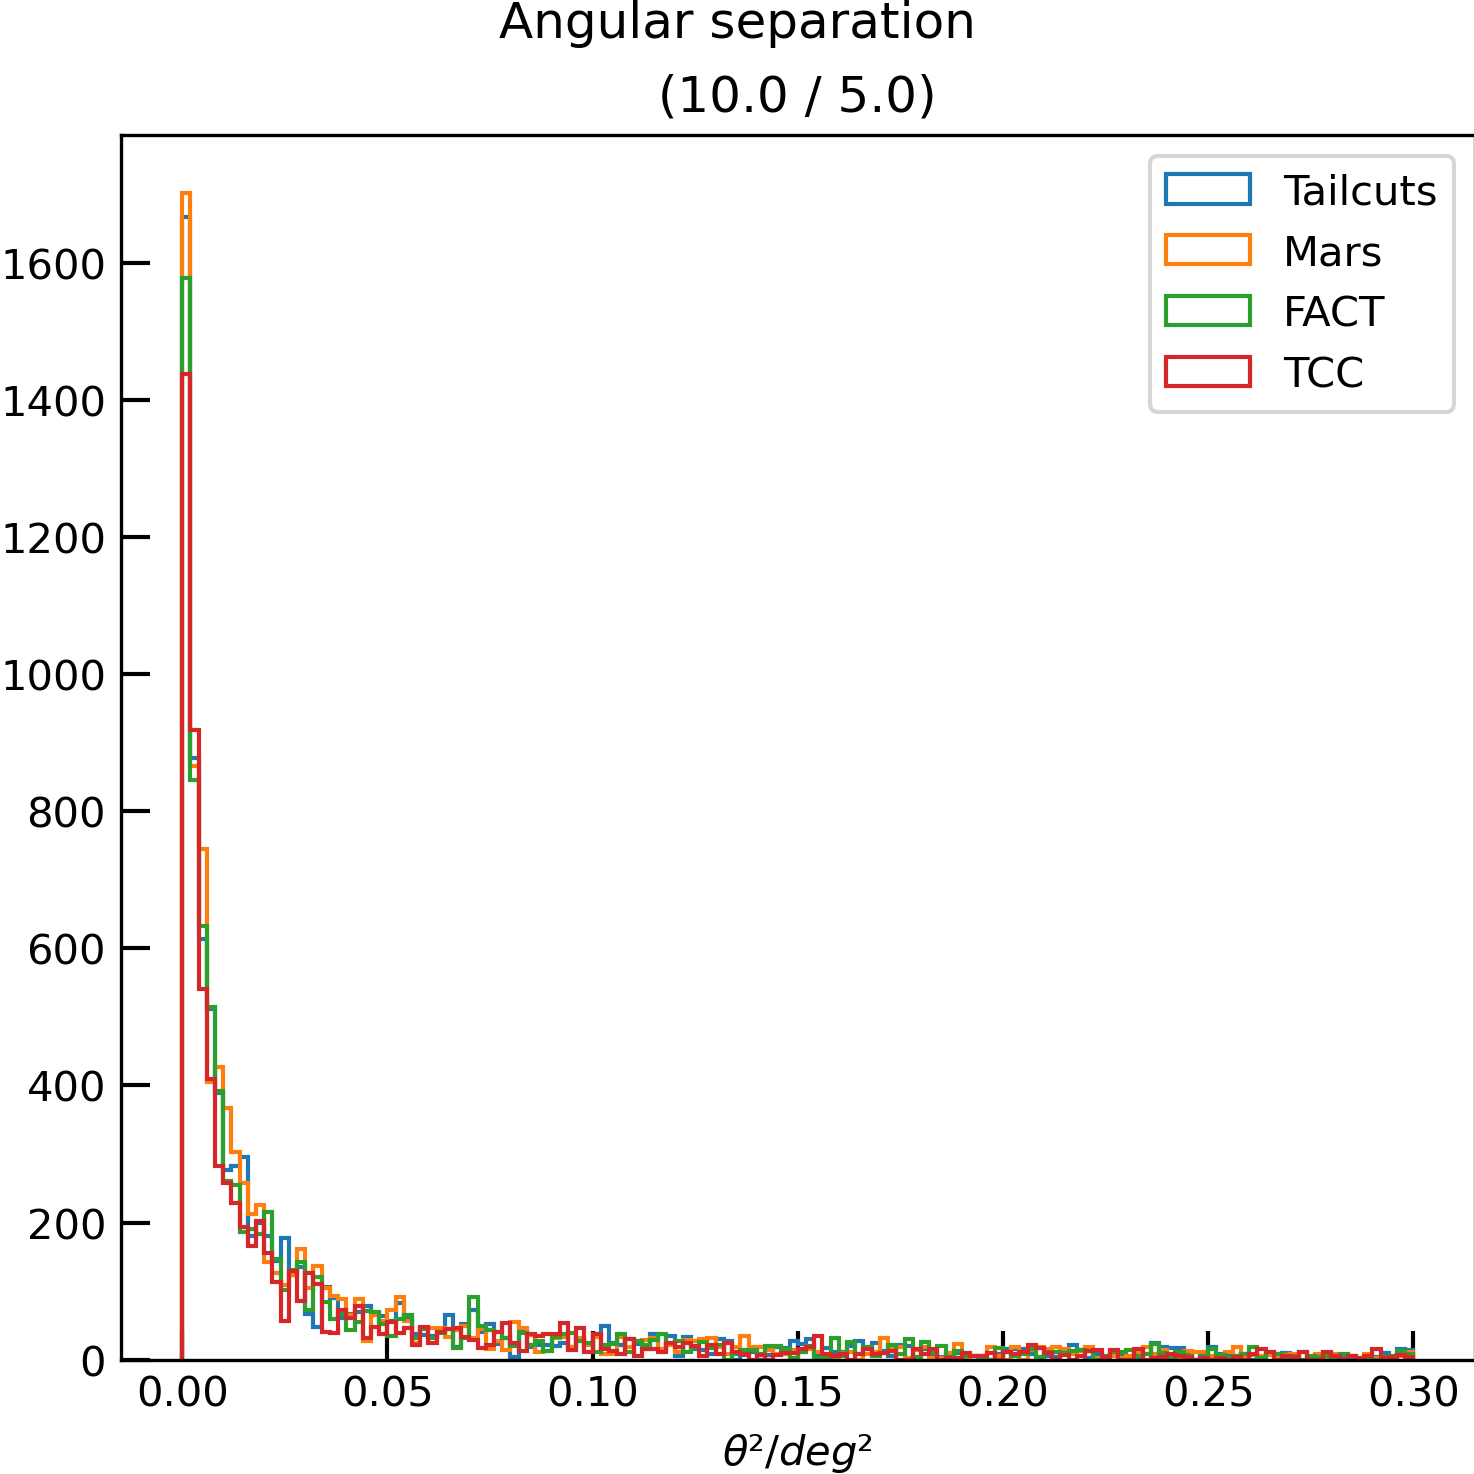
\includegraphics[width=\textwidth]{plots/ang_sep/ang_sep__10.0_5.0_light.png}
    \fi
  \end{minipage}
\end{frame}

\begin{frame}{Angular Resolution}
  \begin{minipage}{0.32\textwidth}
    \ifdefined\darktheme
      \centering
      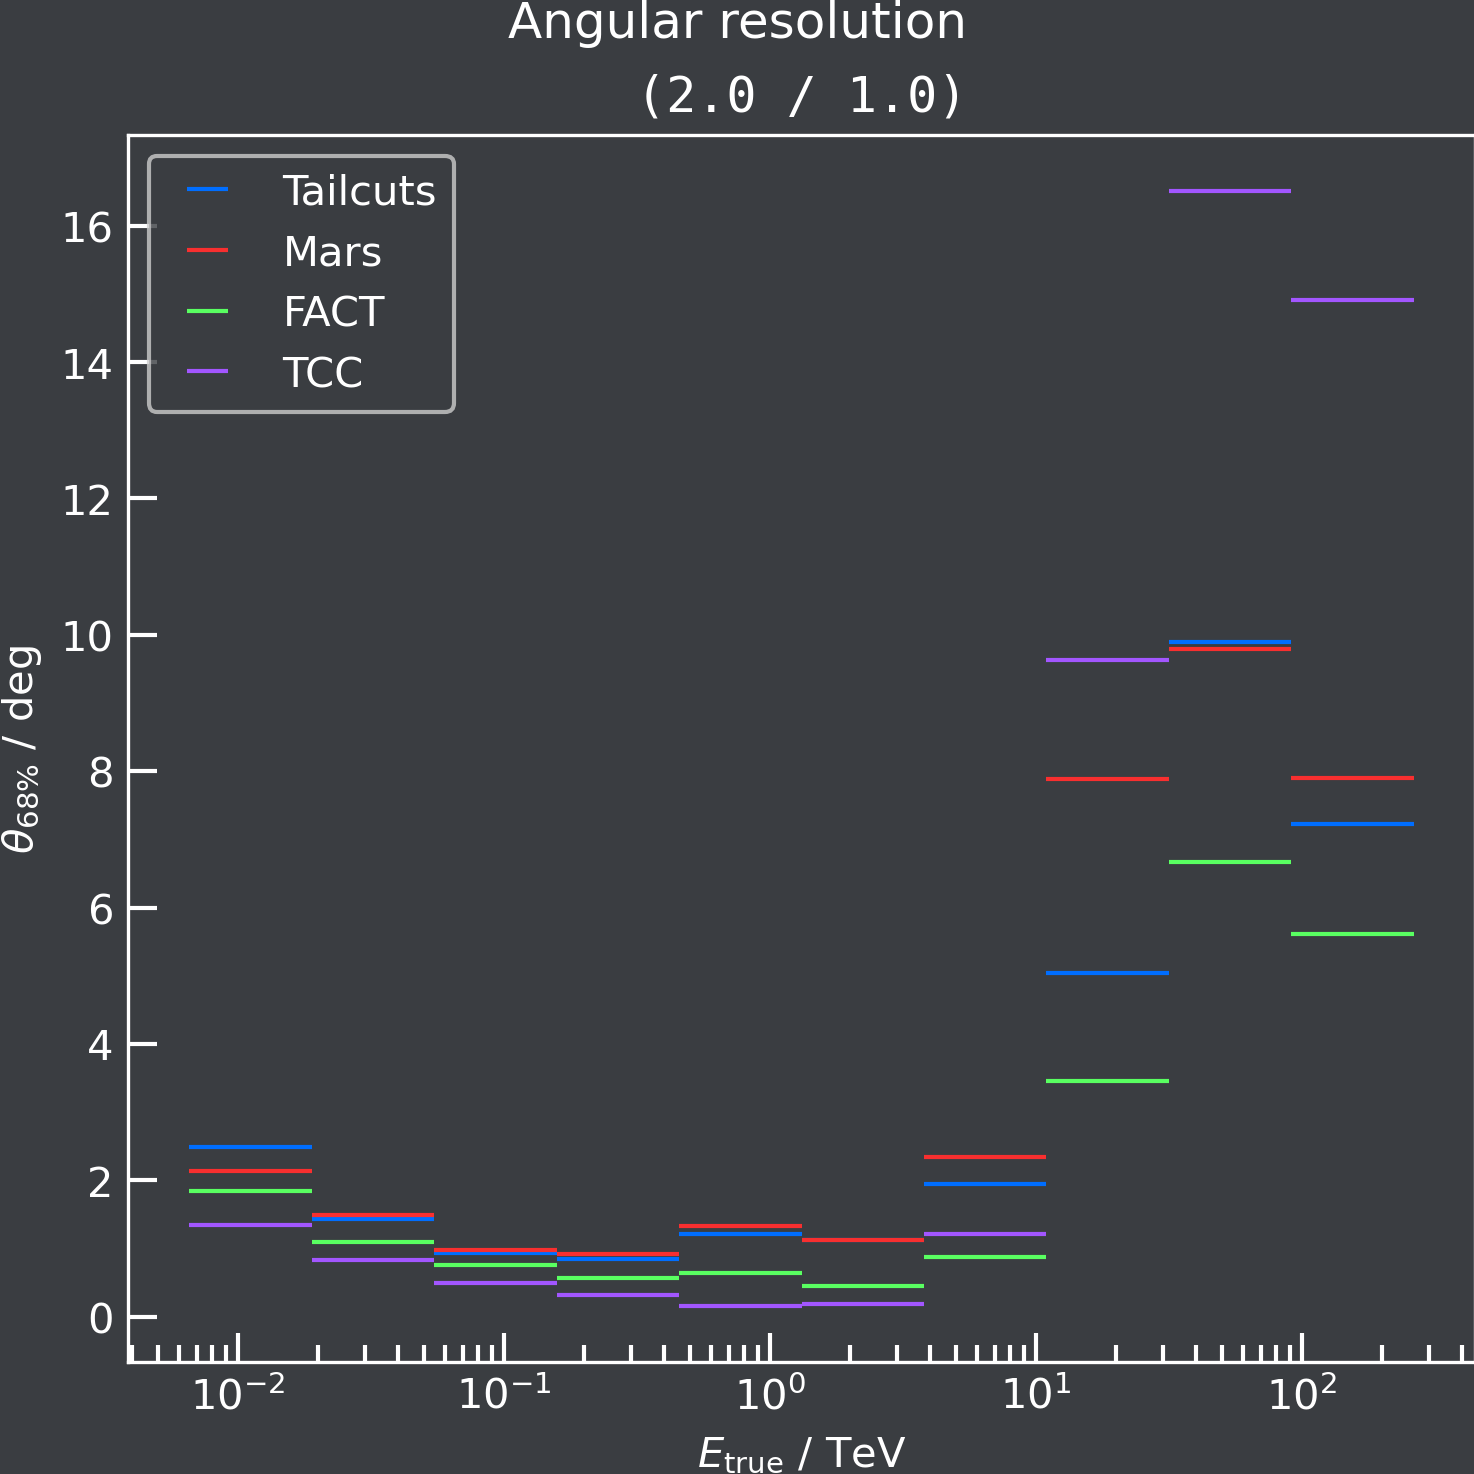
\includegraphics[width=\textwidth]{plots/ang_res/ang_res_2.0_1.0_dark.png}
    \else
      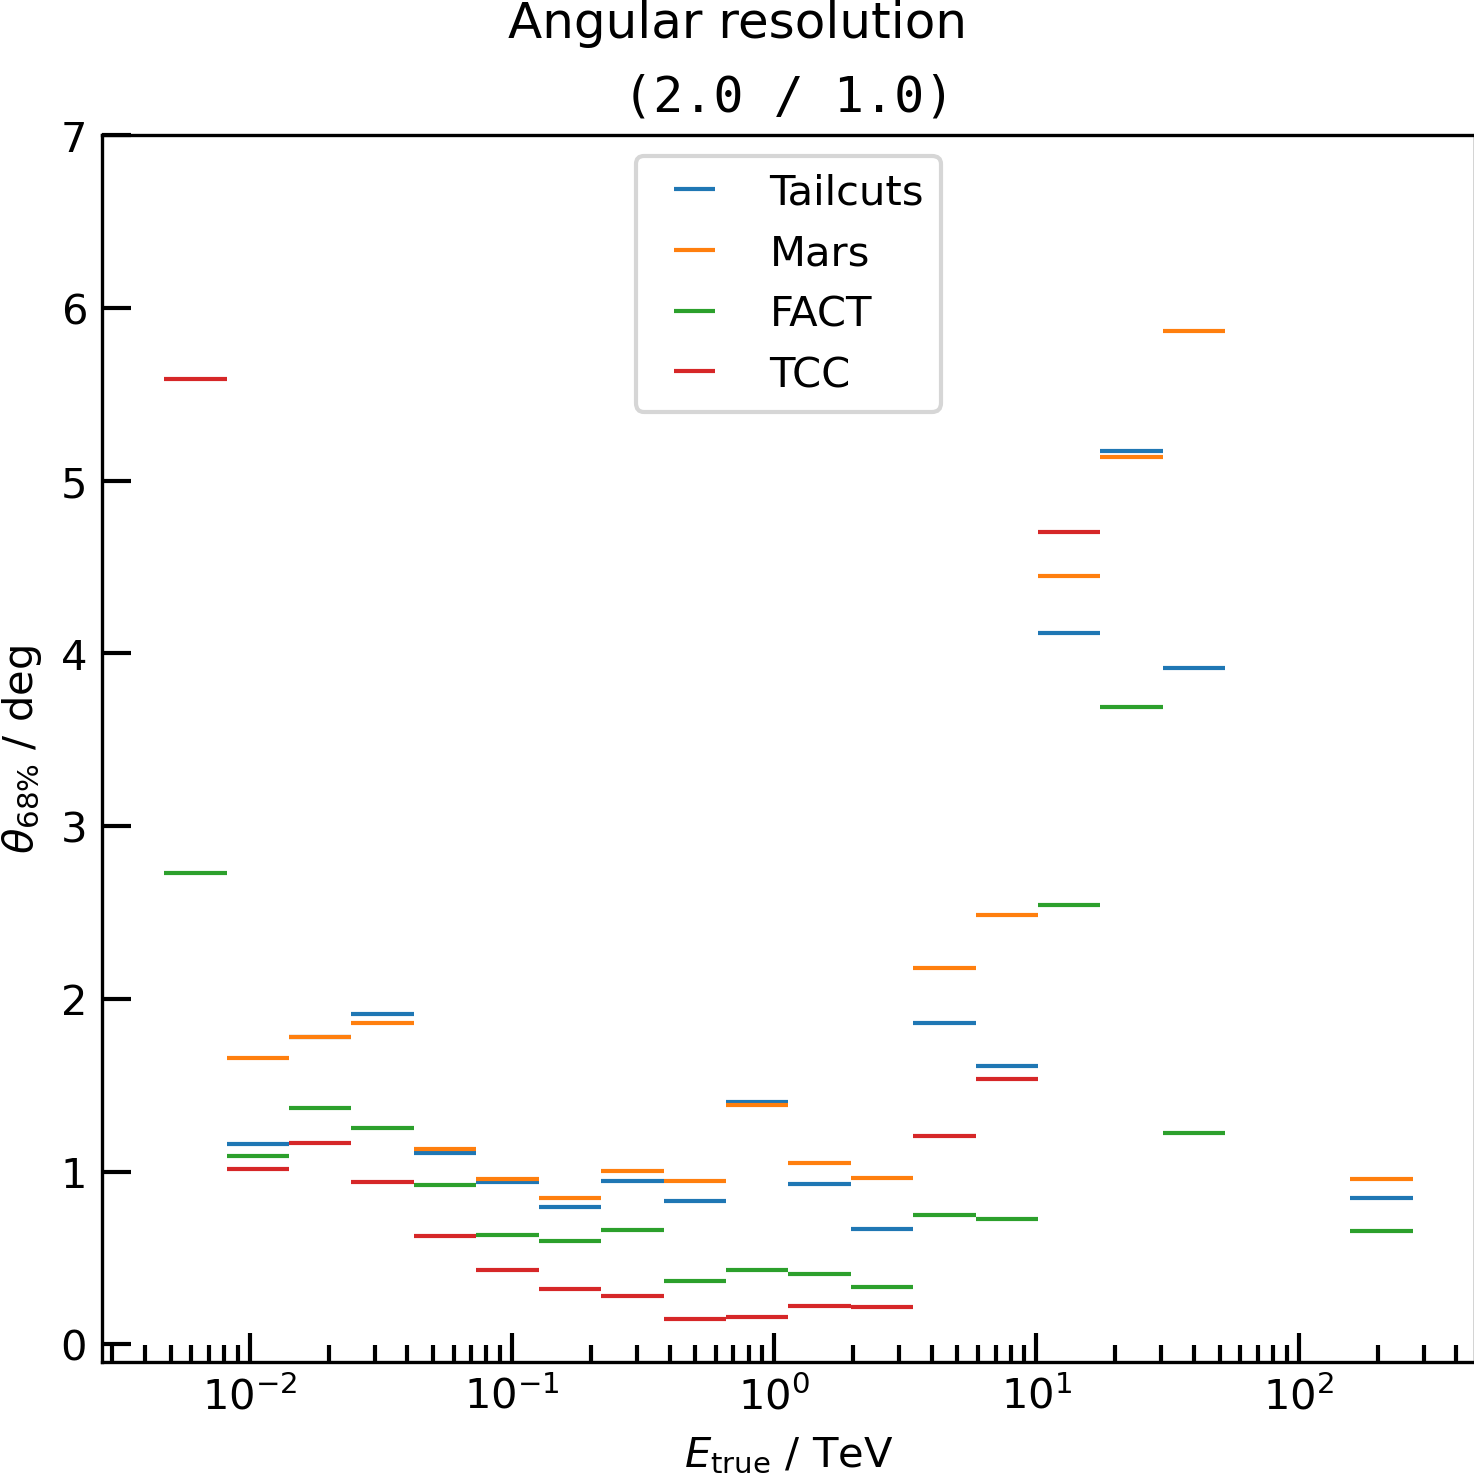
\includegraphics[width=\textwidth]{plots/ang_res/ang_res_2.0_1.0_light.png}
    \fi
  \end{minipage}
  \begin{minipage}{0.32\textwidth}
    \ifdefined\darktheme
      \centering
      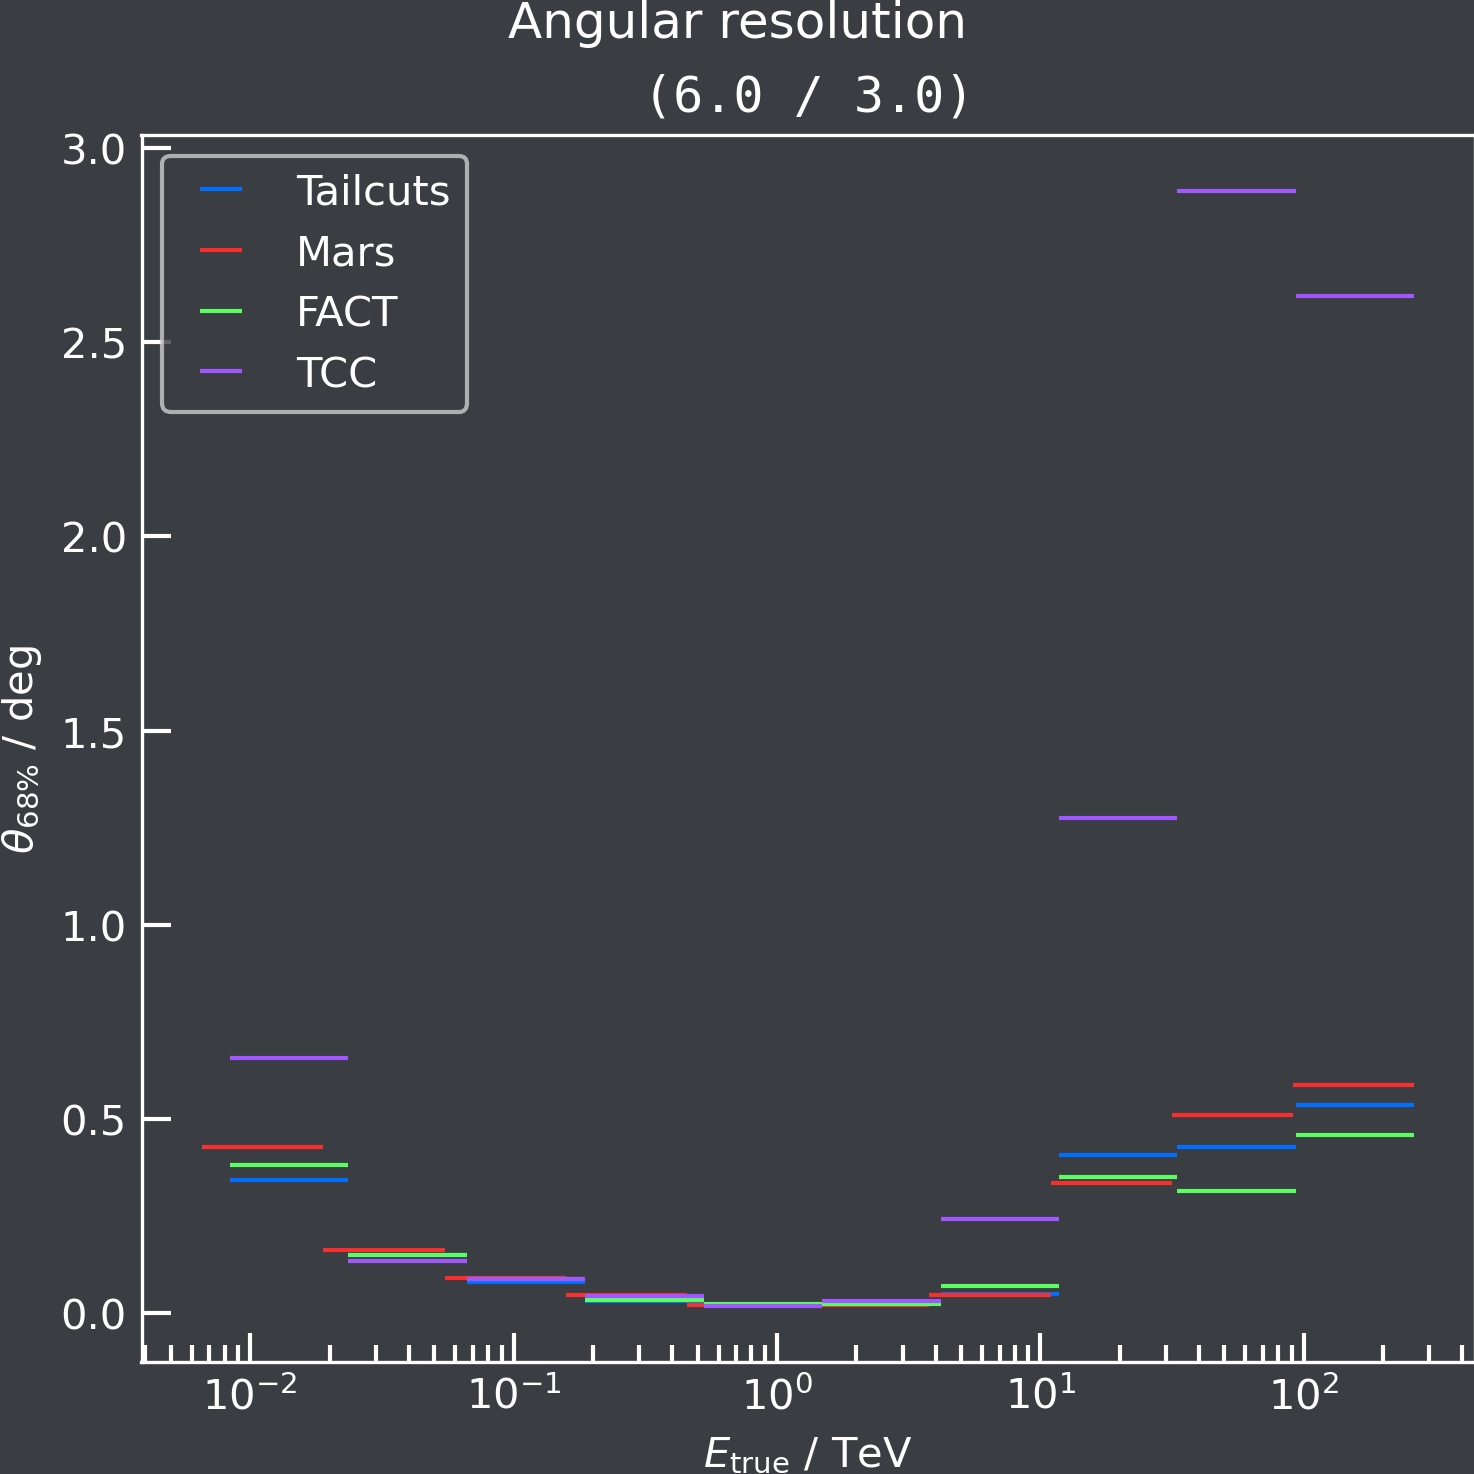
\includegraphics[width=\textwidth]{plots/ang_res/ang_res_6.0_3.0_dark.png}
    \else
      \centering
      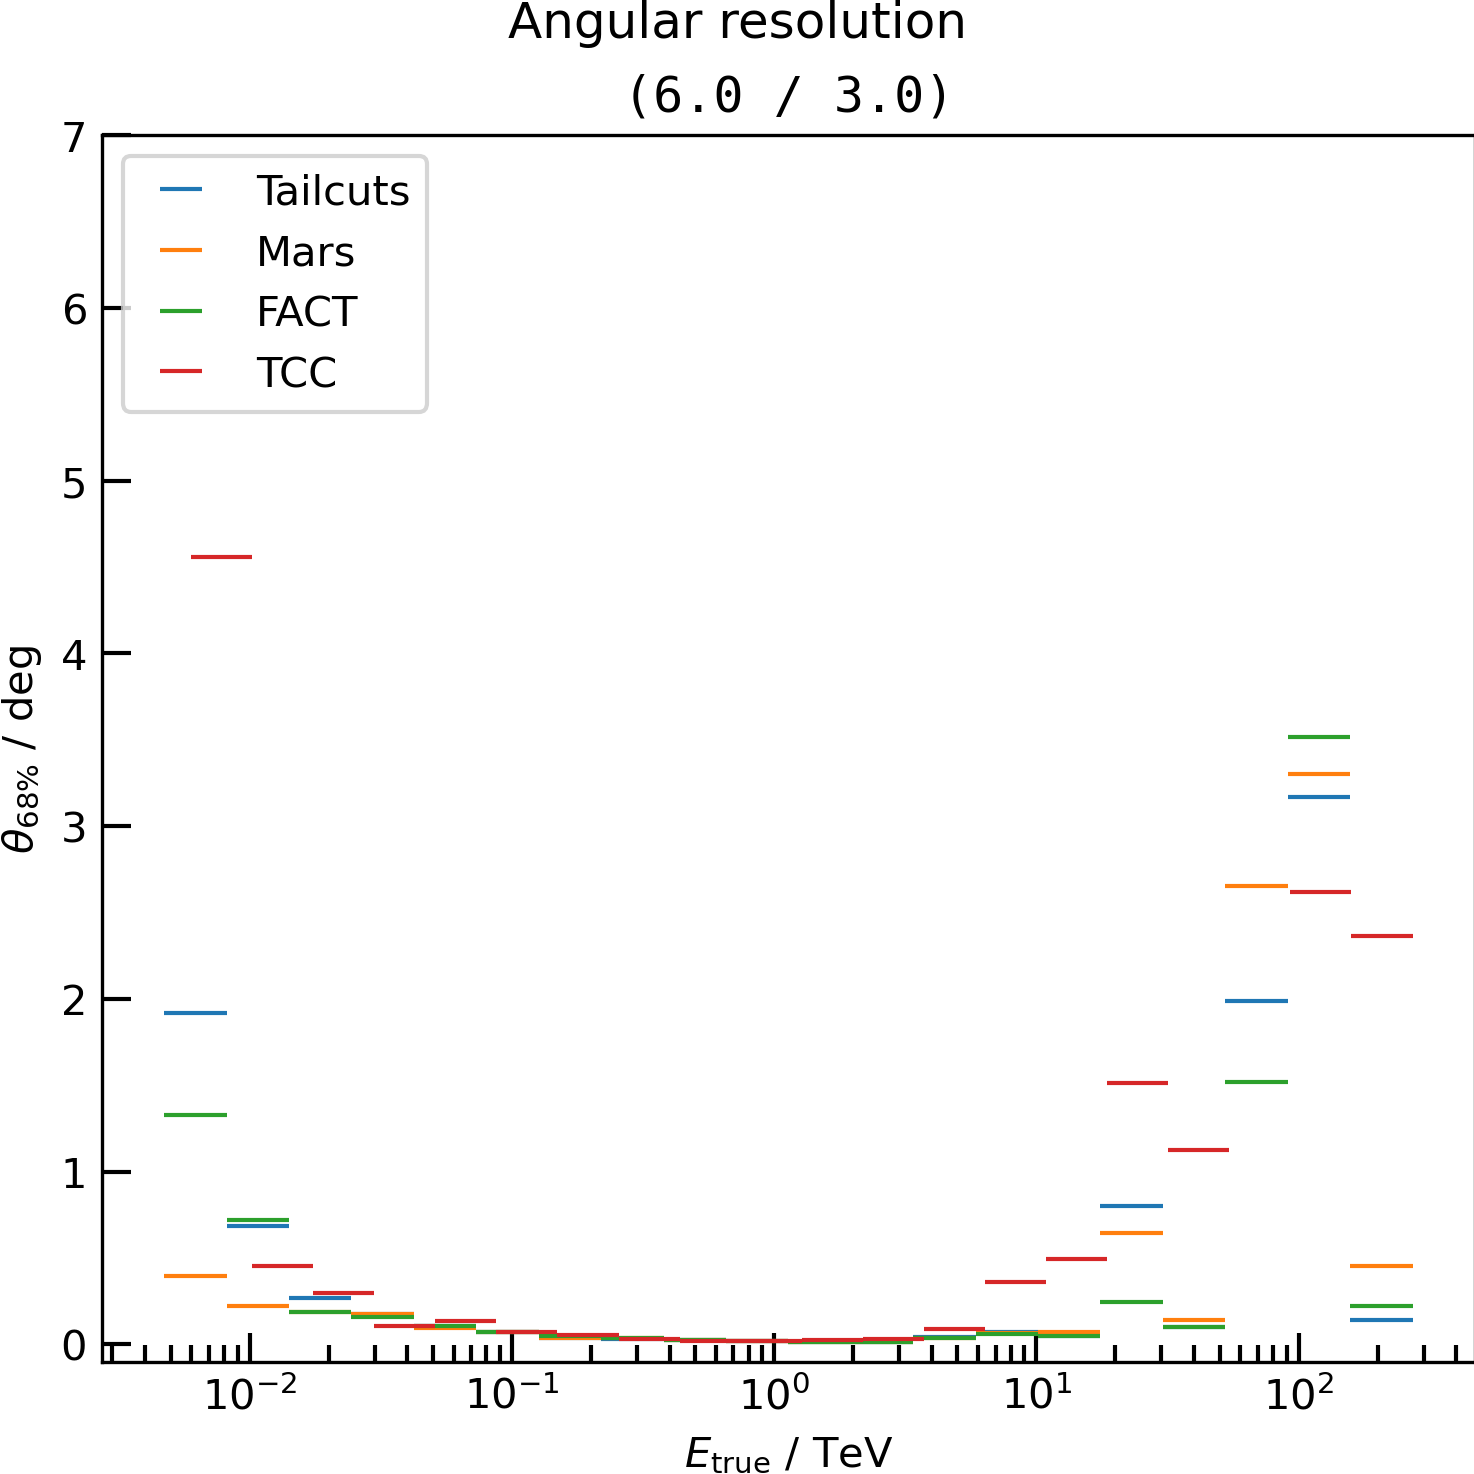
\includegraphics[width=\textwidth]{plots/ang_res/ang_res_6.0_3.0_light.png}
    \fi
  \end{minipage}
  \begin{minipage}{0.32\textwidth}
    \ifdefined\darktheme
      \centering
      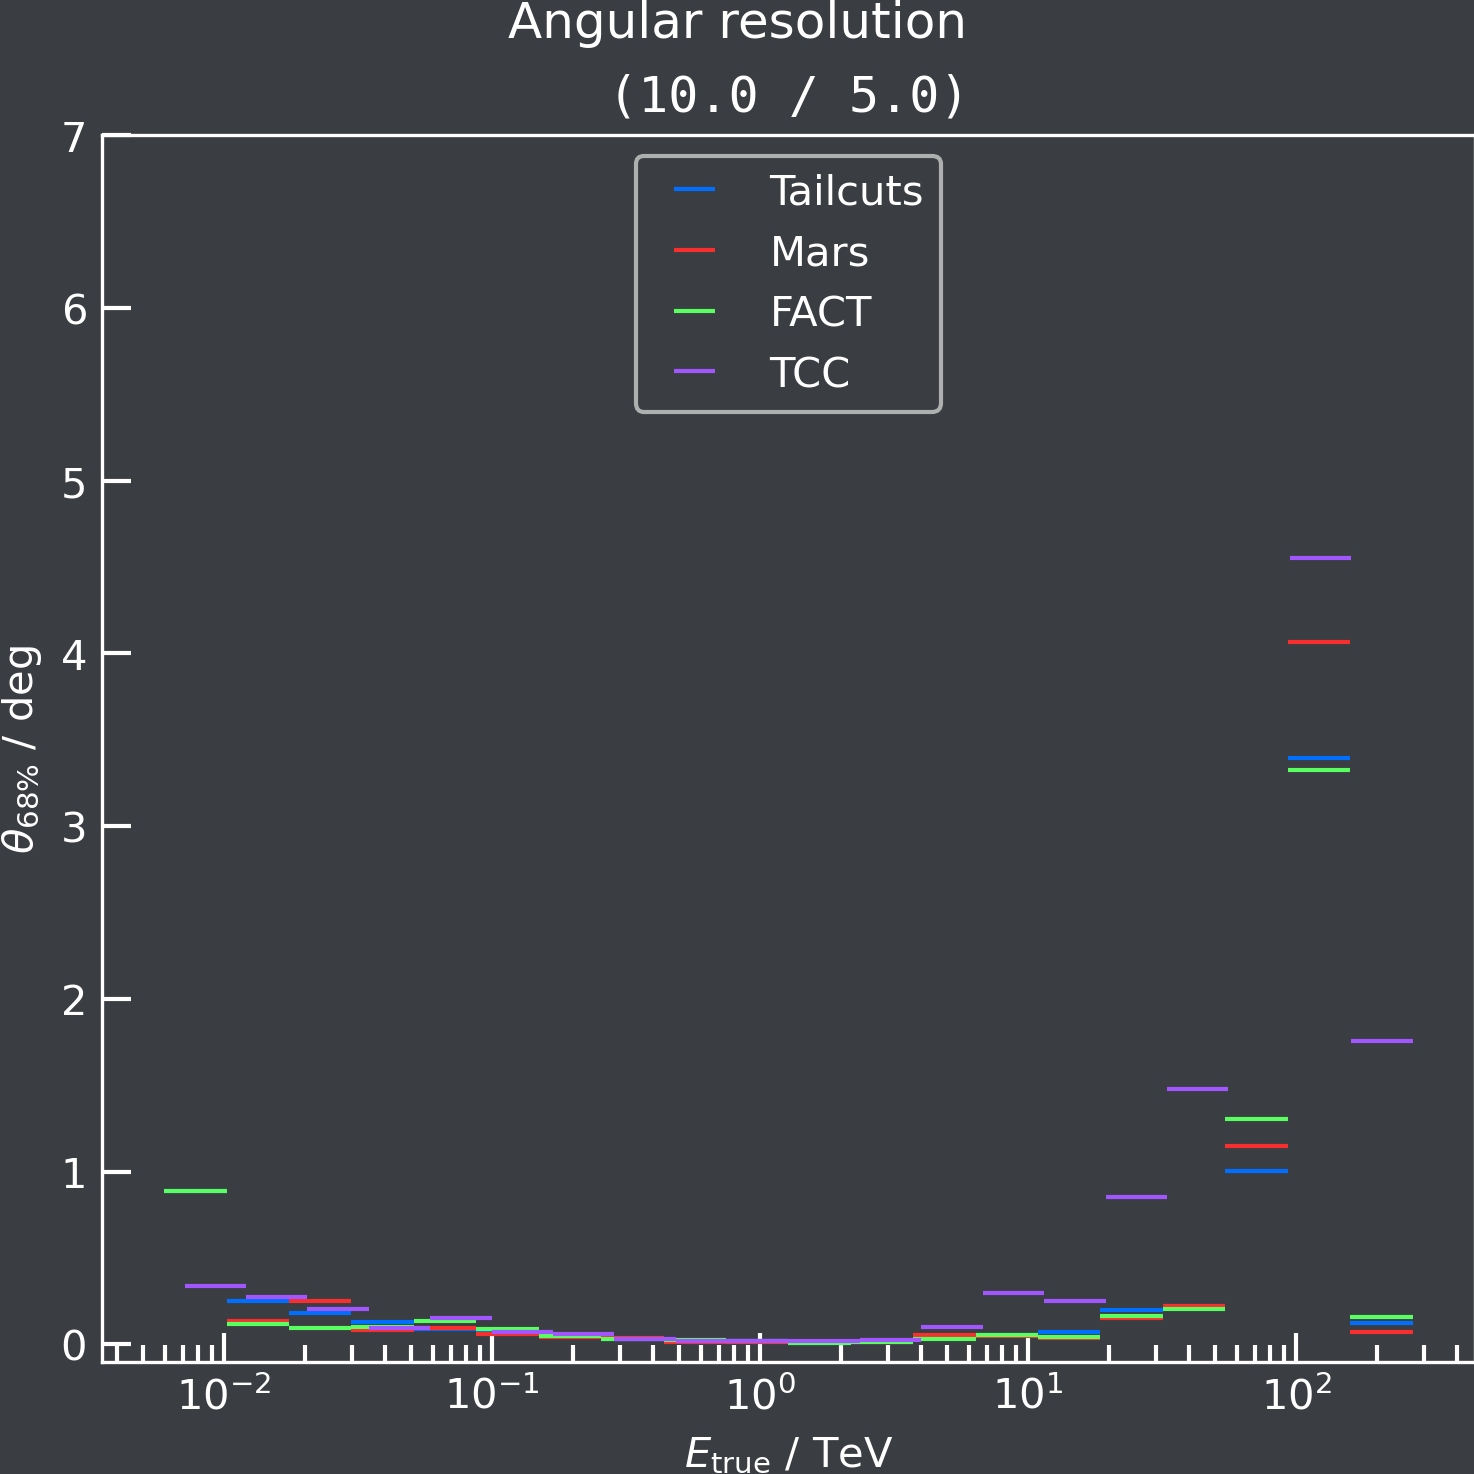
\includegraphics[width=\textwidth]{plots/ang_res/ang_res_10.0_5.0_dark.png}
    \else
      \centering
      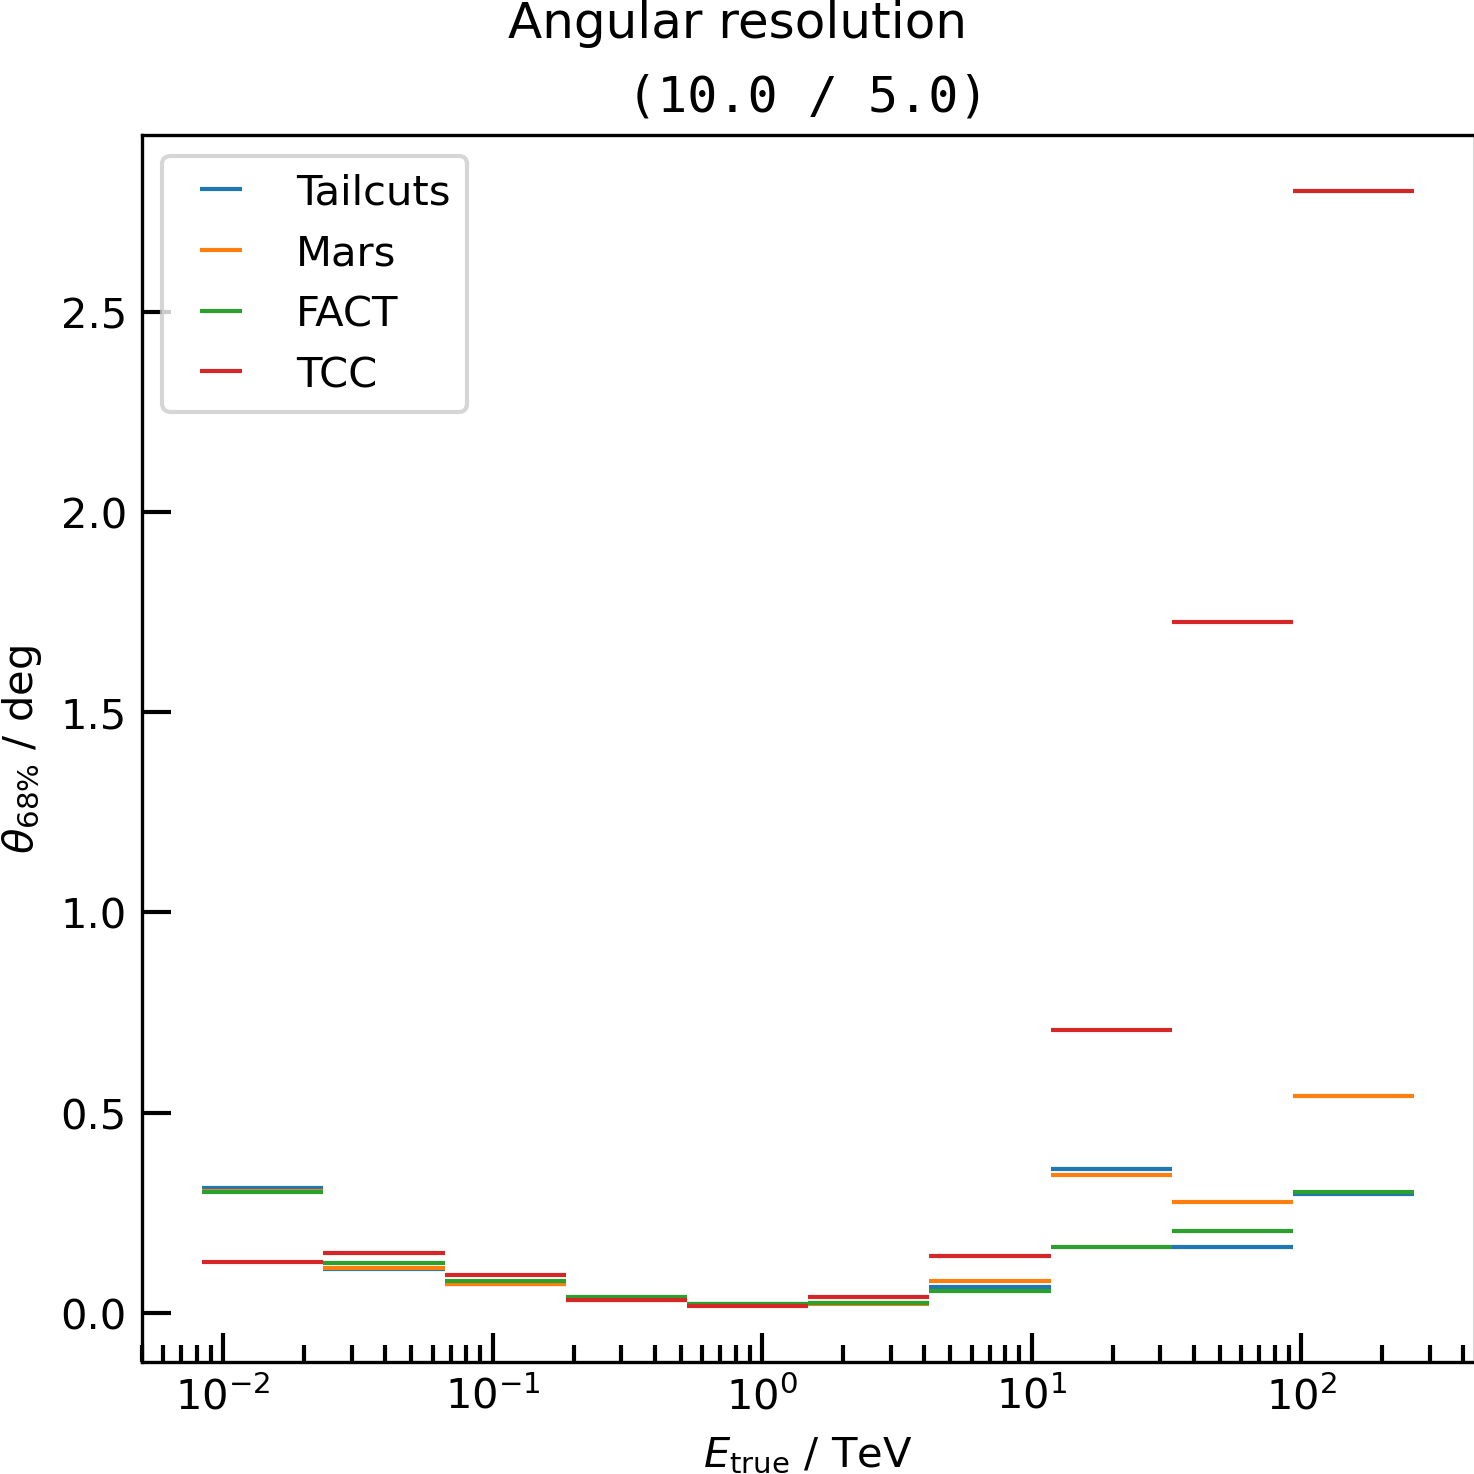
\includegraphics[width=\textwidth]{plots/ang_res/ang_res_10.0_5.0_light.png}
    \fi
  \end{minipage}
\end{frame}

\subsection{ROC Curves}
\begin{frame}{ROC curves and precision and recall curves}
  \ifdefined\darktheme
    \centering
    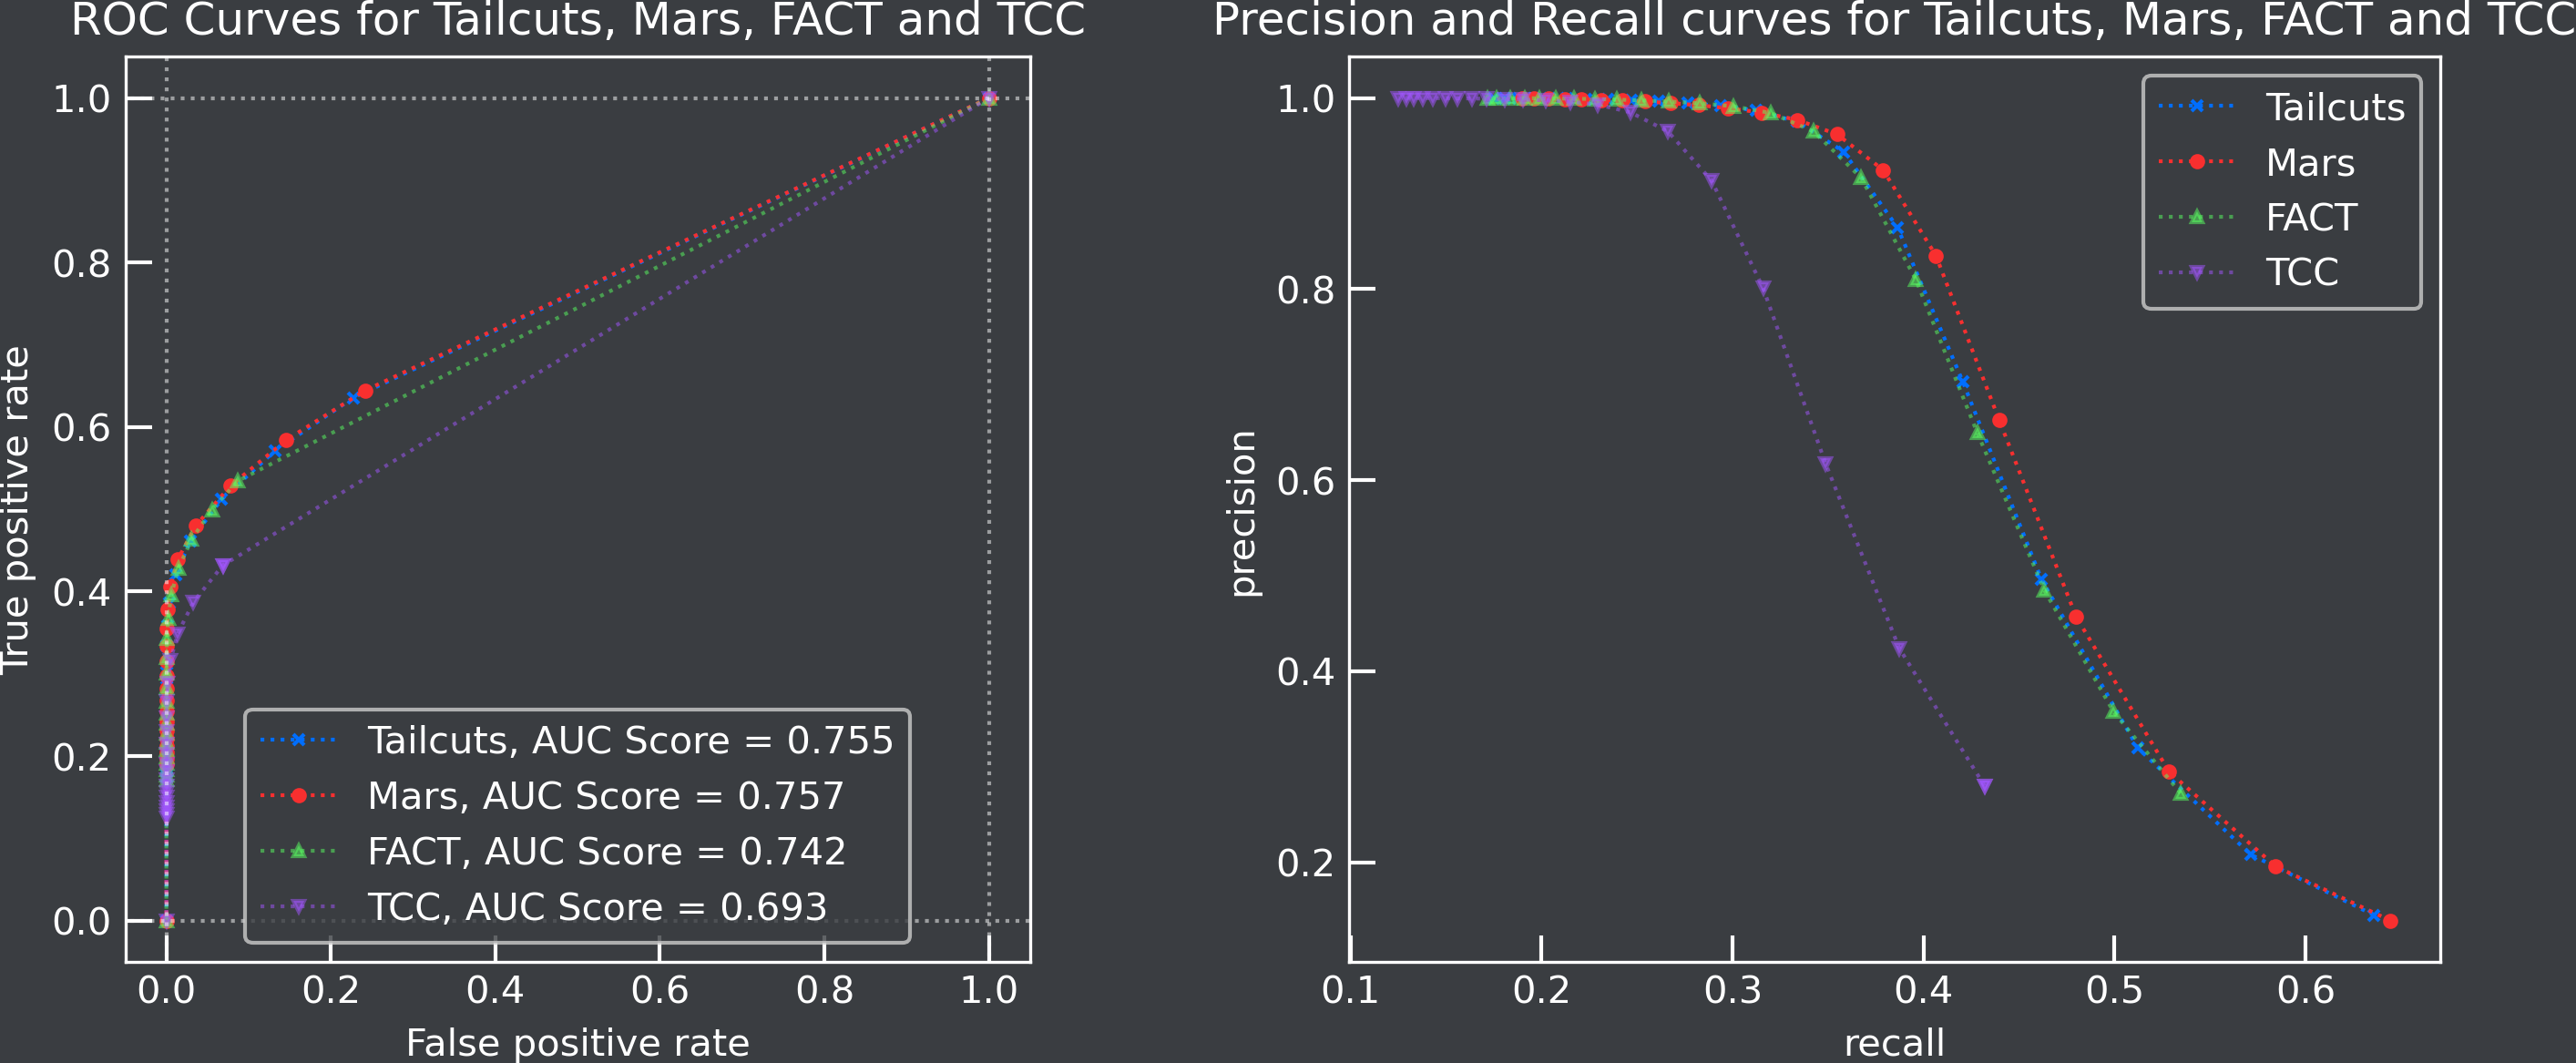
\includegraphics[width=\textwidth]{plots/roc_prec_rec_duo_dark.png}
  \else
    \centering
    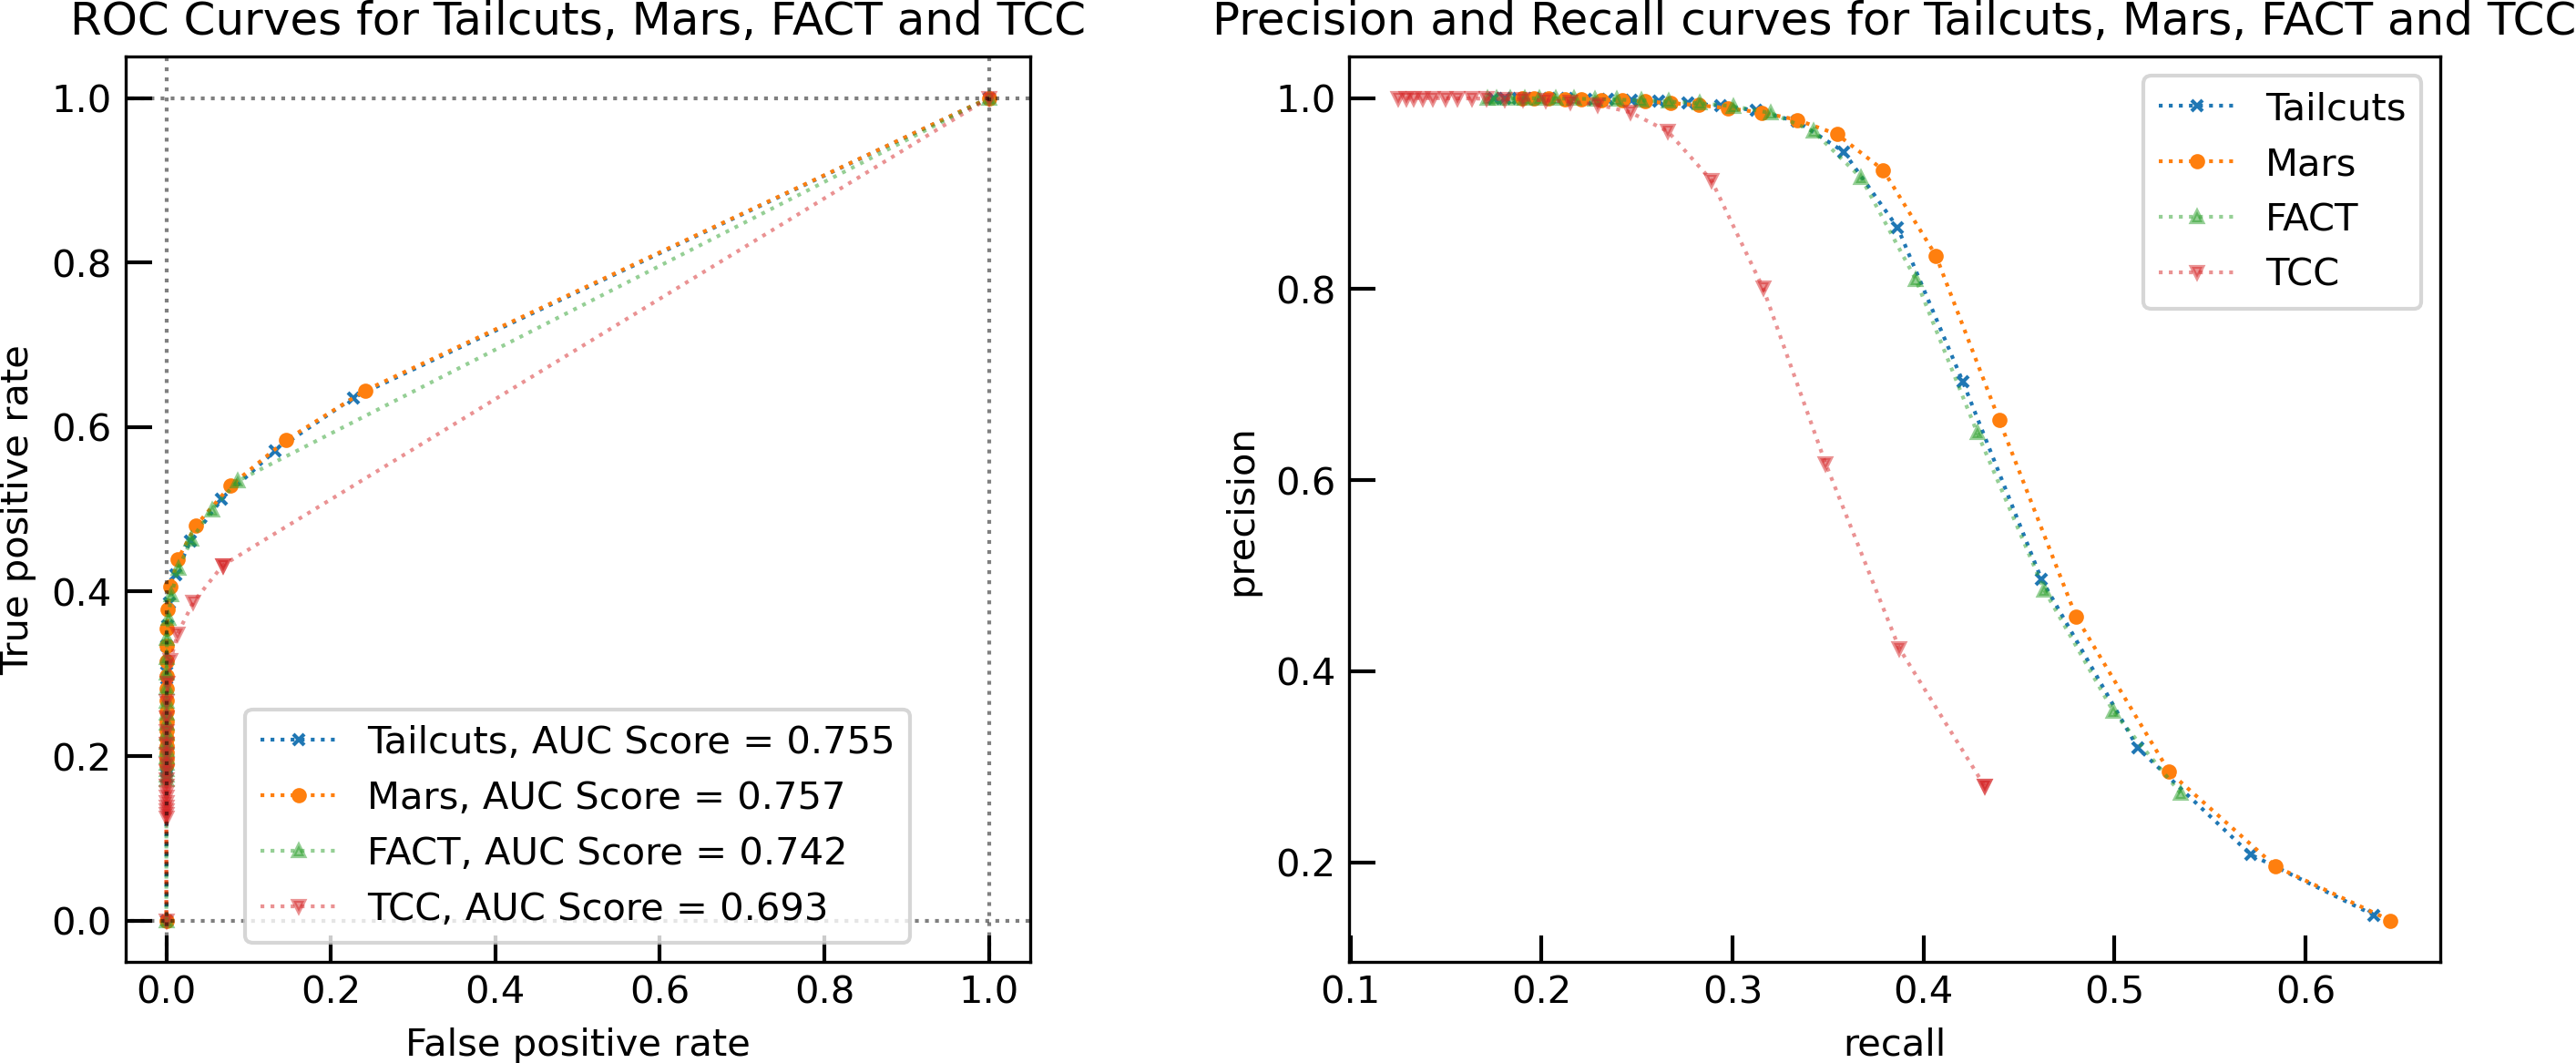
\includegraphics[width=\textwidth]{plots/roc_prec_rec_duo_light.png}
  \fi
\end{frame}
\begin{frame}{Picture Thresholds}
  \ifdefined\darktheme
    \centering
    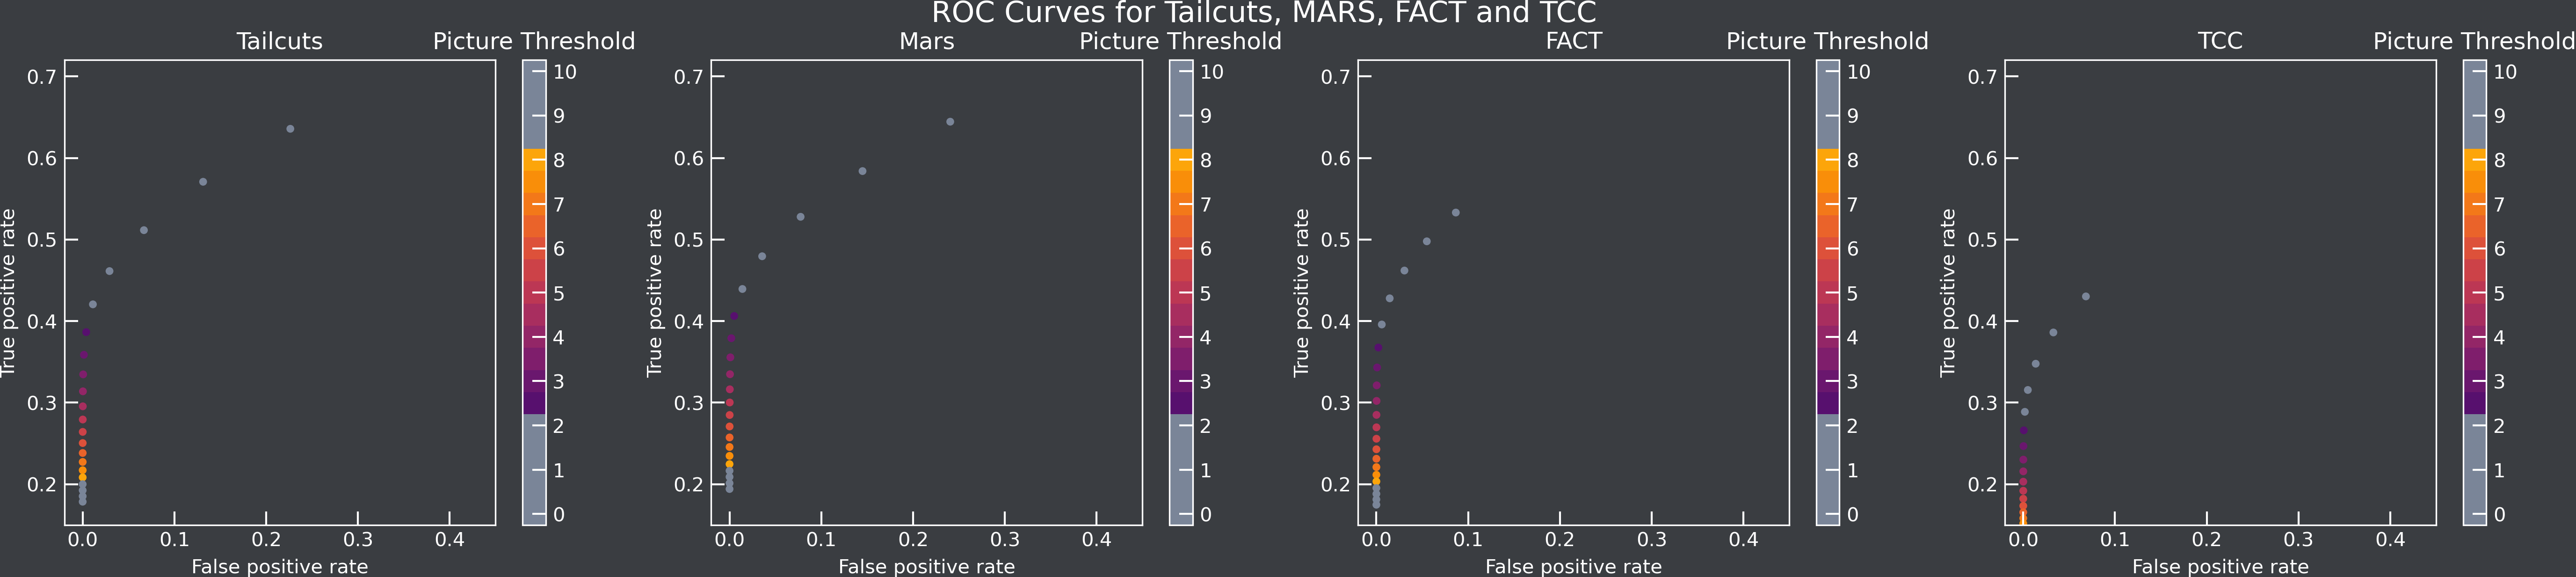
\includegraphics[width=\textwidth]{plots/pic_thresh_roc_dark.png}
  \else
    \centering
    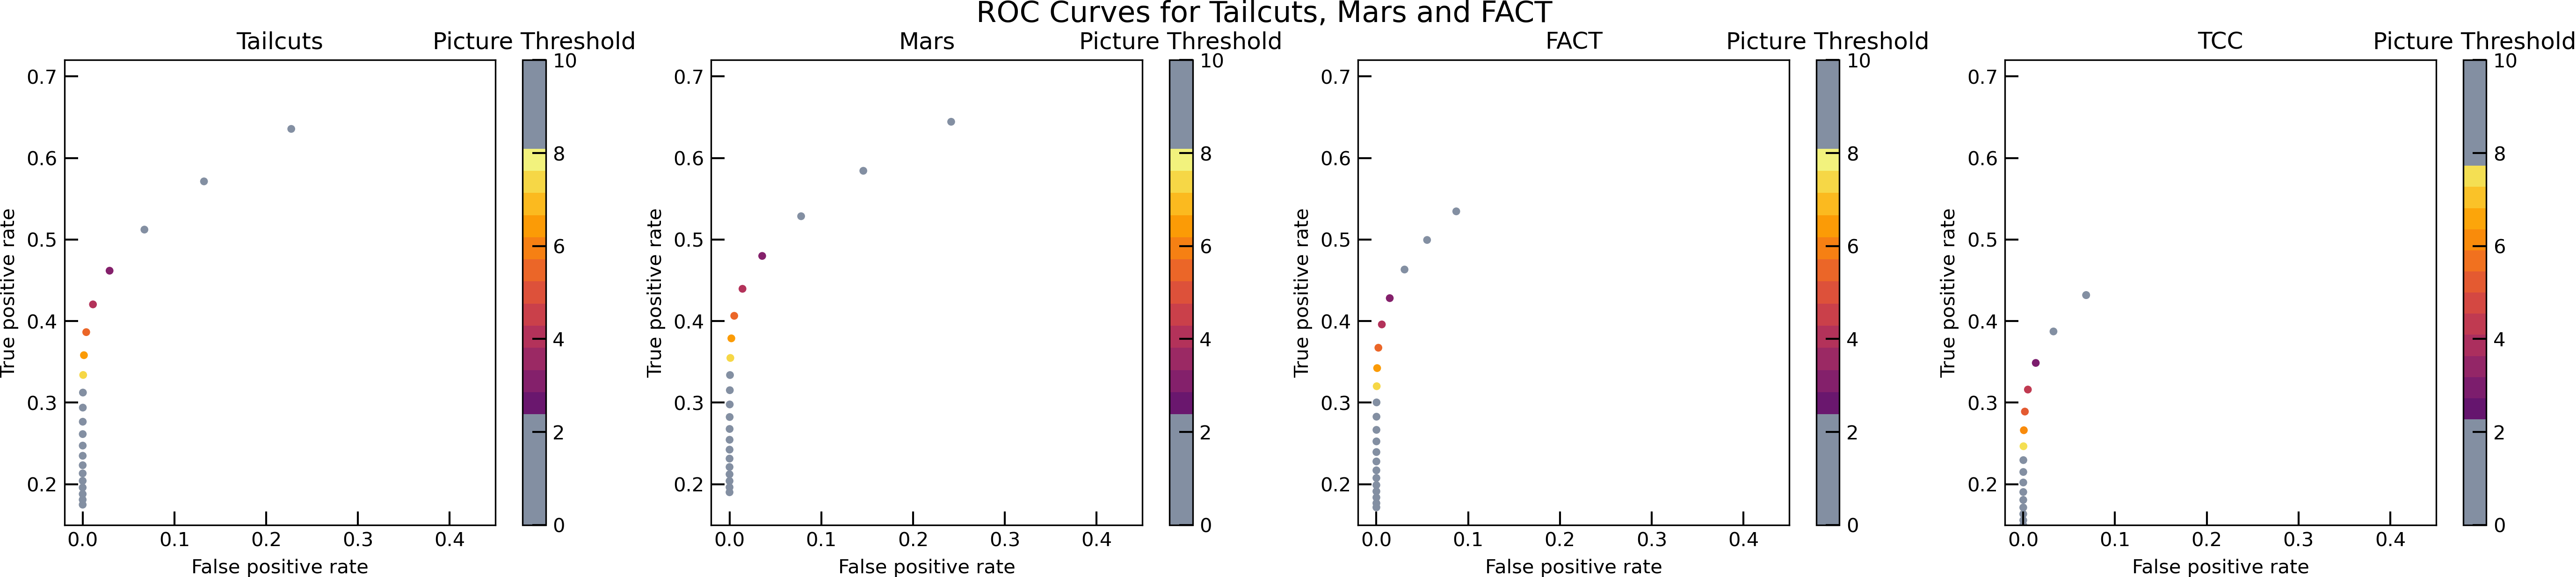
\includegraphics[width=\textwidth]{plots/pic_thresh_roc_light.png}
  \fi
\end{frame}

\subsection{Ratio of Surviving Pixels}
\begin{frame}{Ratio of Surviving Pixels}
  \ifdefined\darktheme
    \centering
    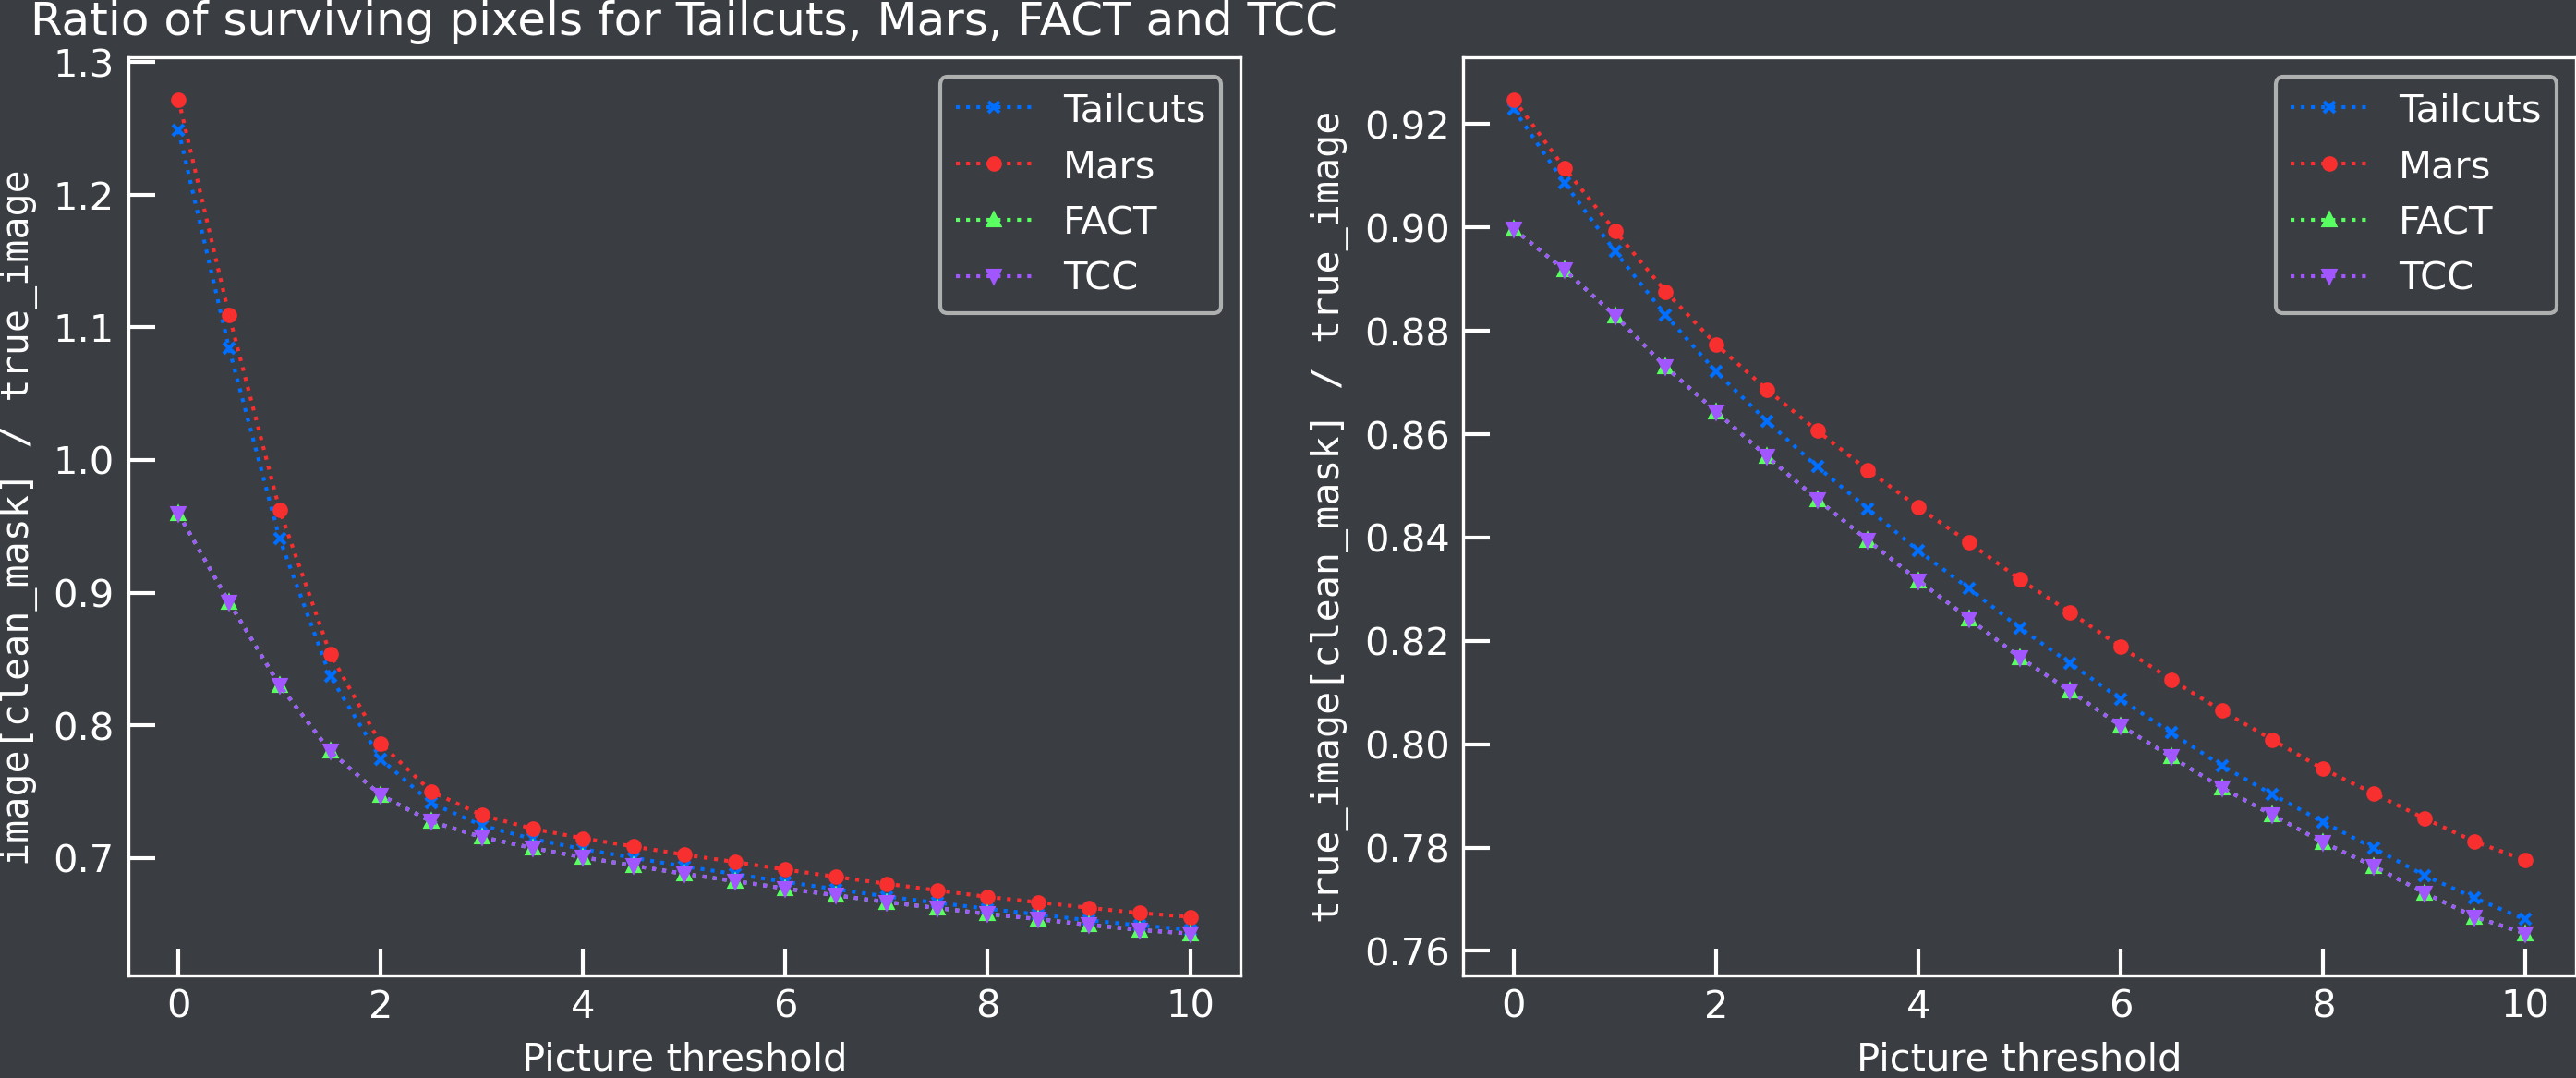
\includegraphics[width=\textwidth]{plots/surv_pixels_dark.png}
  \else
    \centering
    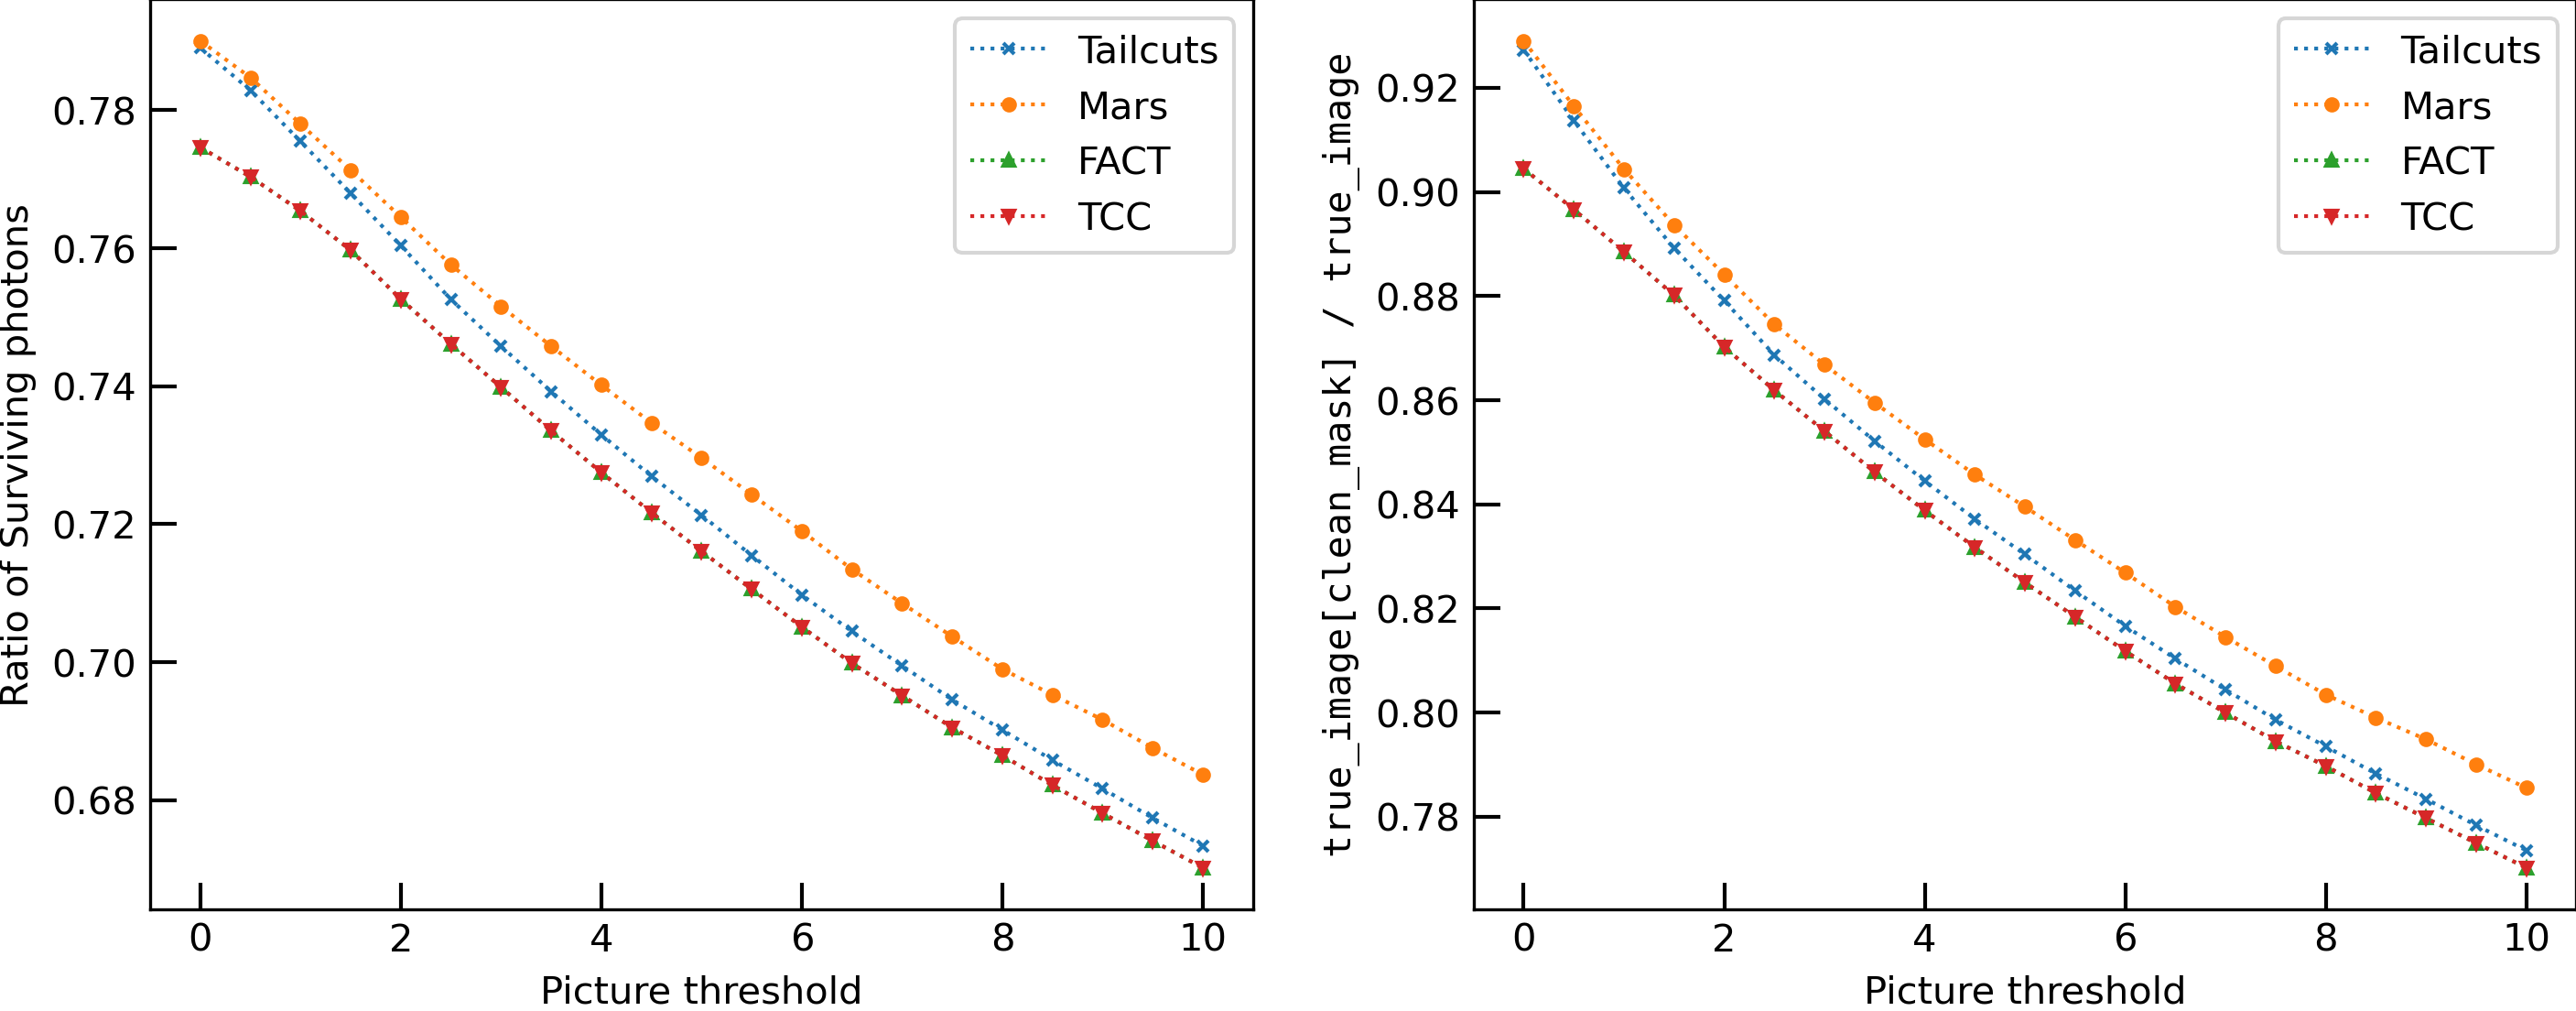
\includegraphics[width=\textwidth]{plots/surv_pixels_light.png}
  \fi
\end{frame}

\subsection{Metrics}
\begin{frame}{Metrics}
  \only<1>{
    \ifdefined\darktheme
      \centering
      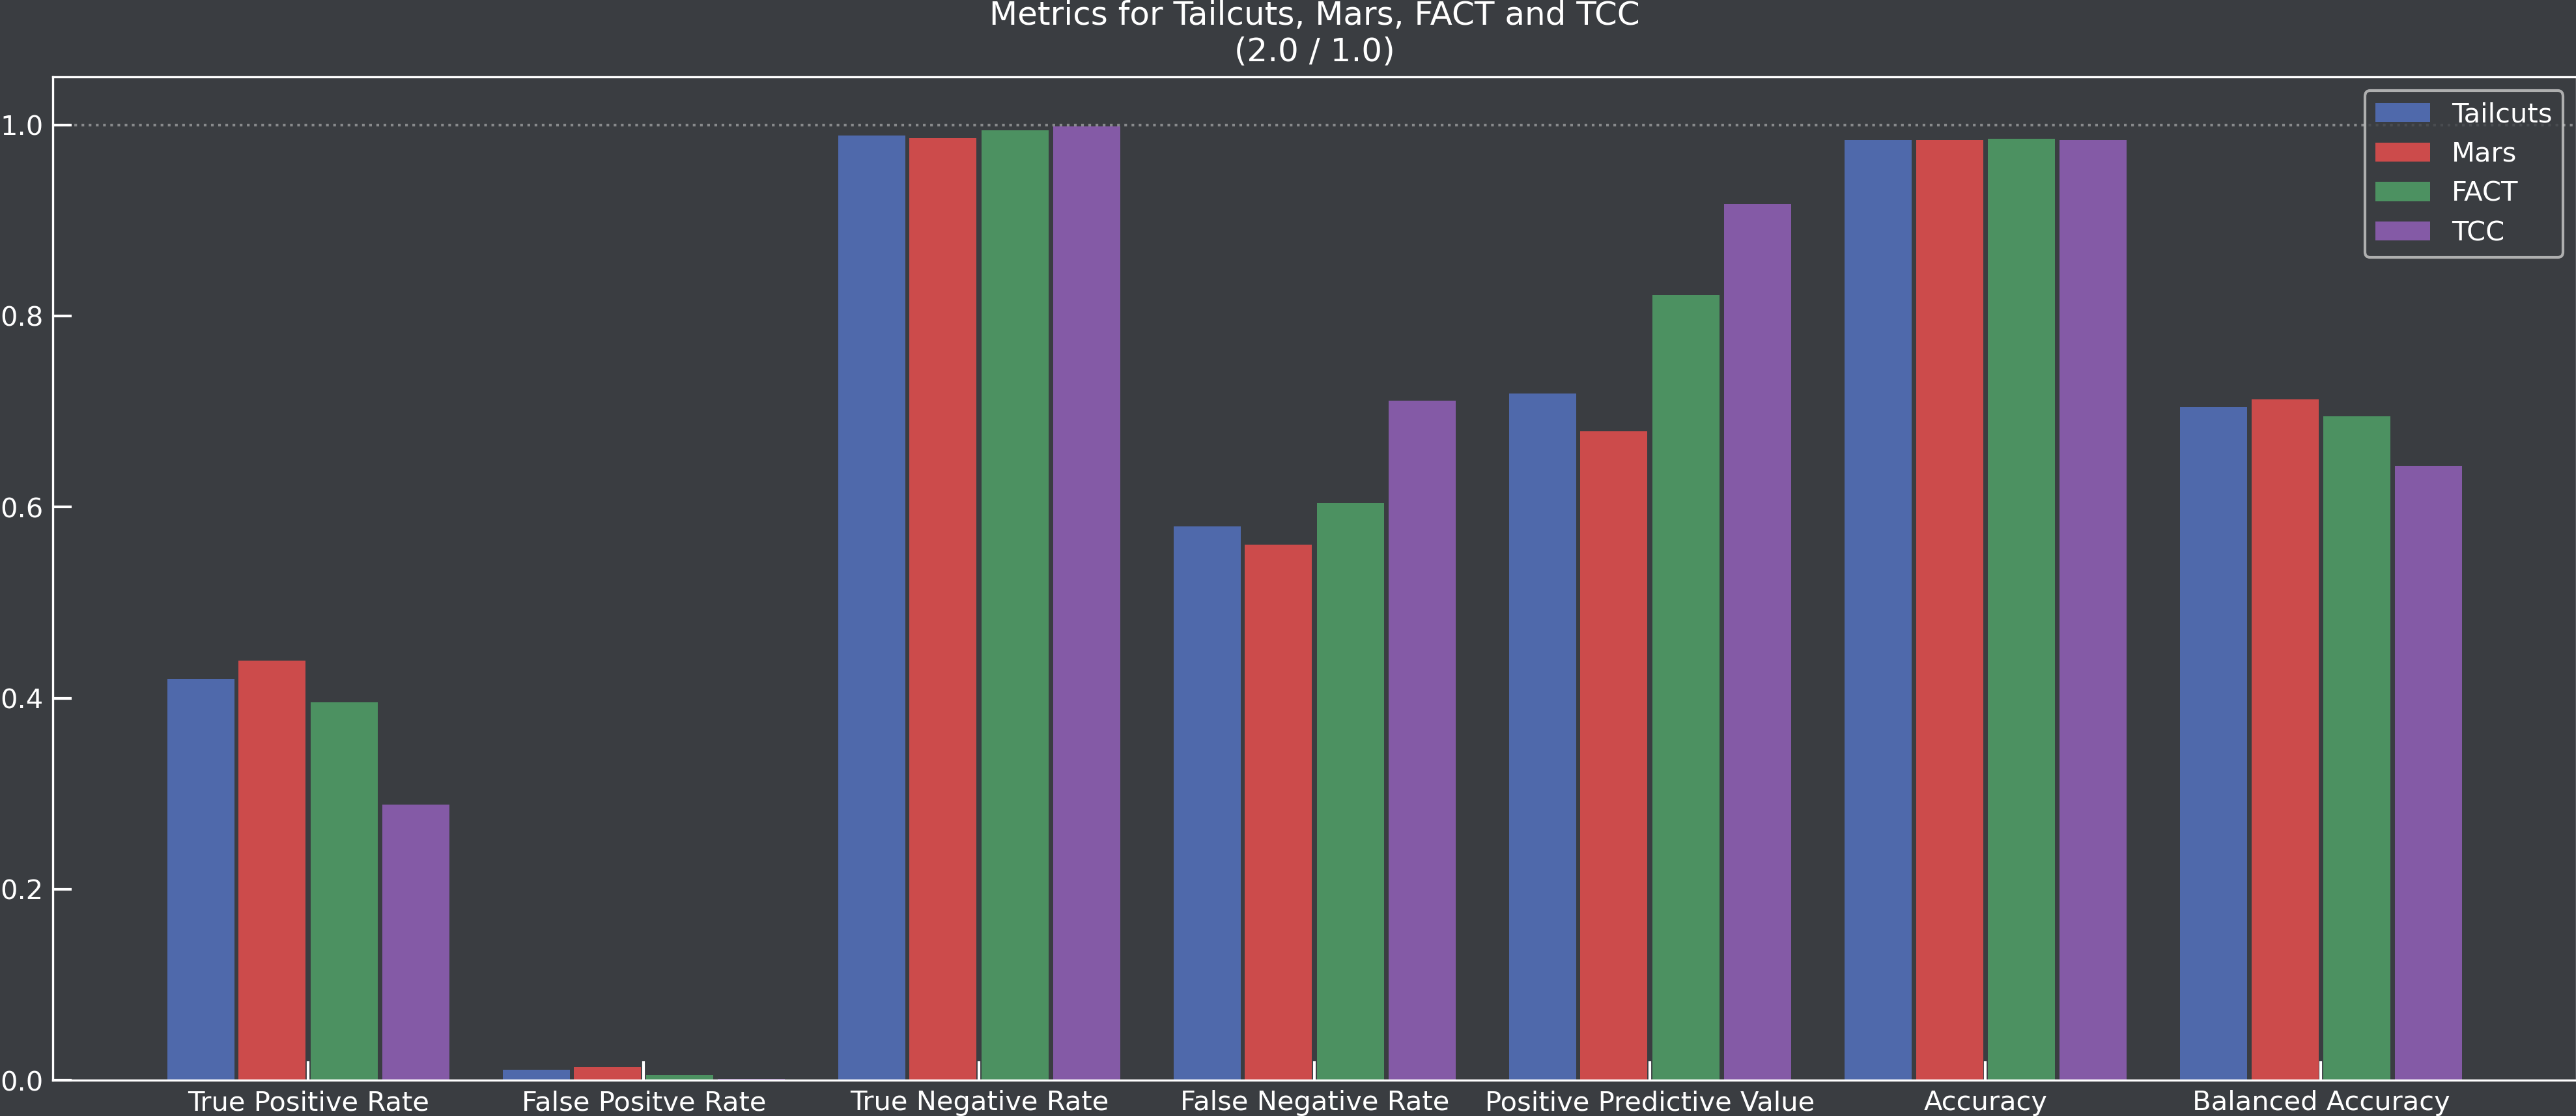
\includegraphics[width=\textwidth]{plots/metrics/metrics_2.0_1.0_dark.png}
    \else
      \centering
      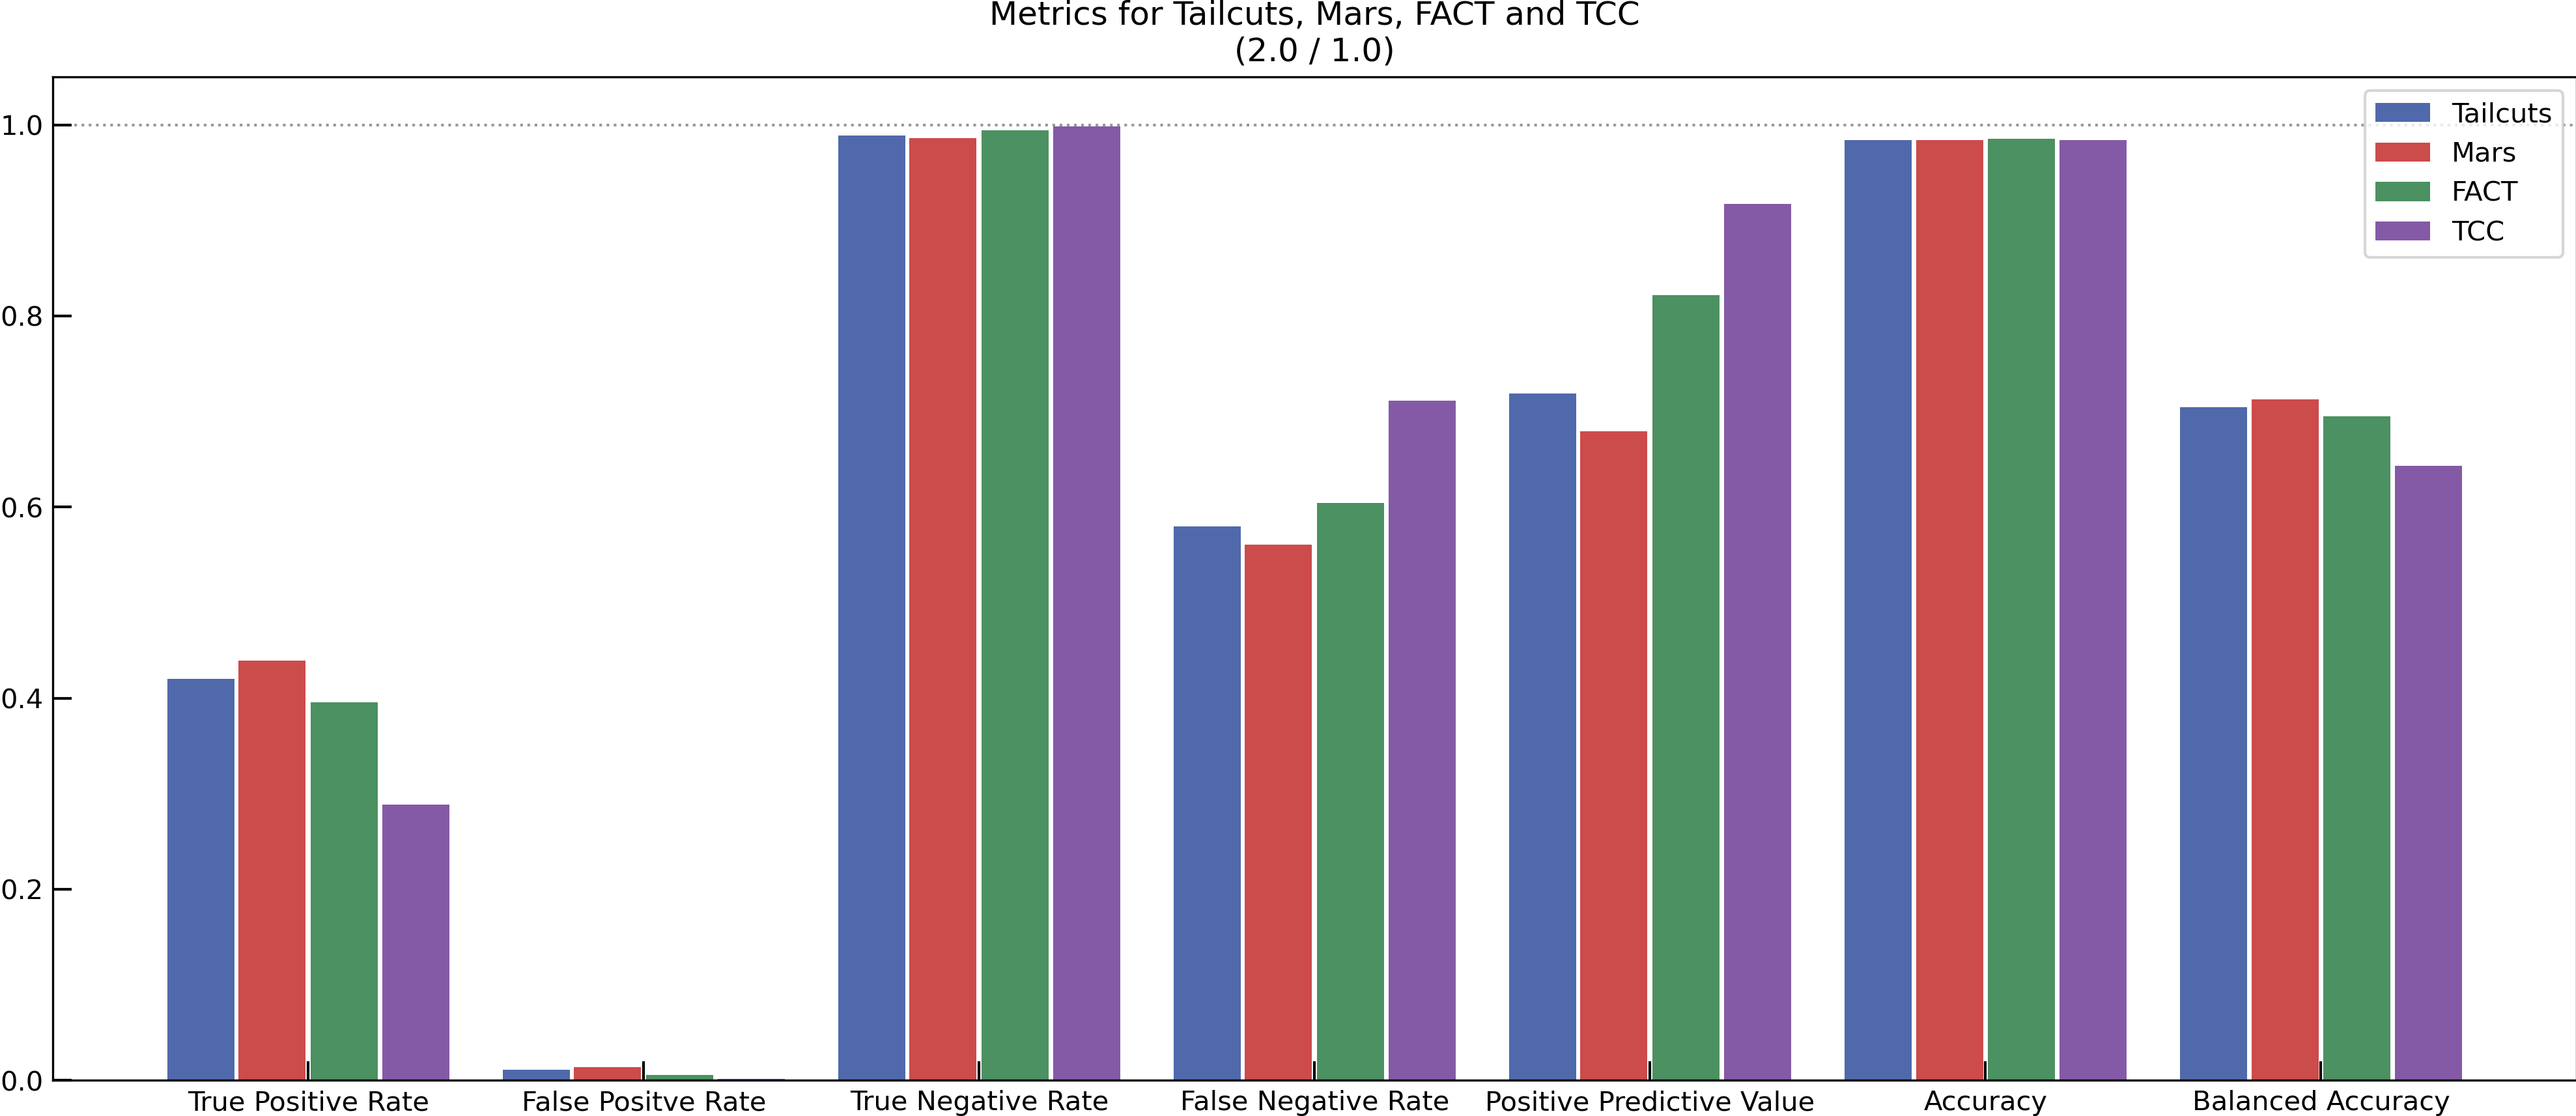
\includegraphics[width=\textwidth]{plots/metrics/metrics_2.0_1.0_light.png}
    \fi
  }
  \only<2>{
    \ifdefined\darktheme
      \centering
      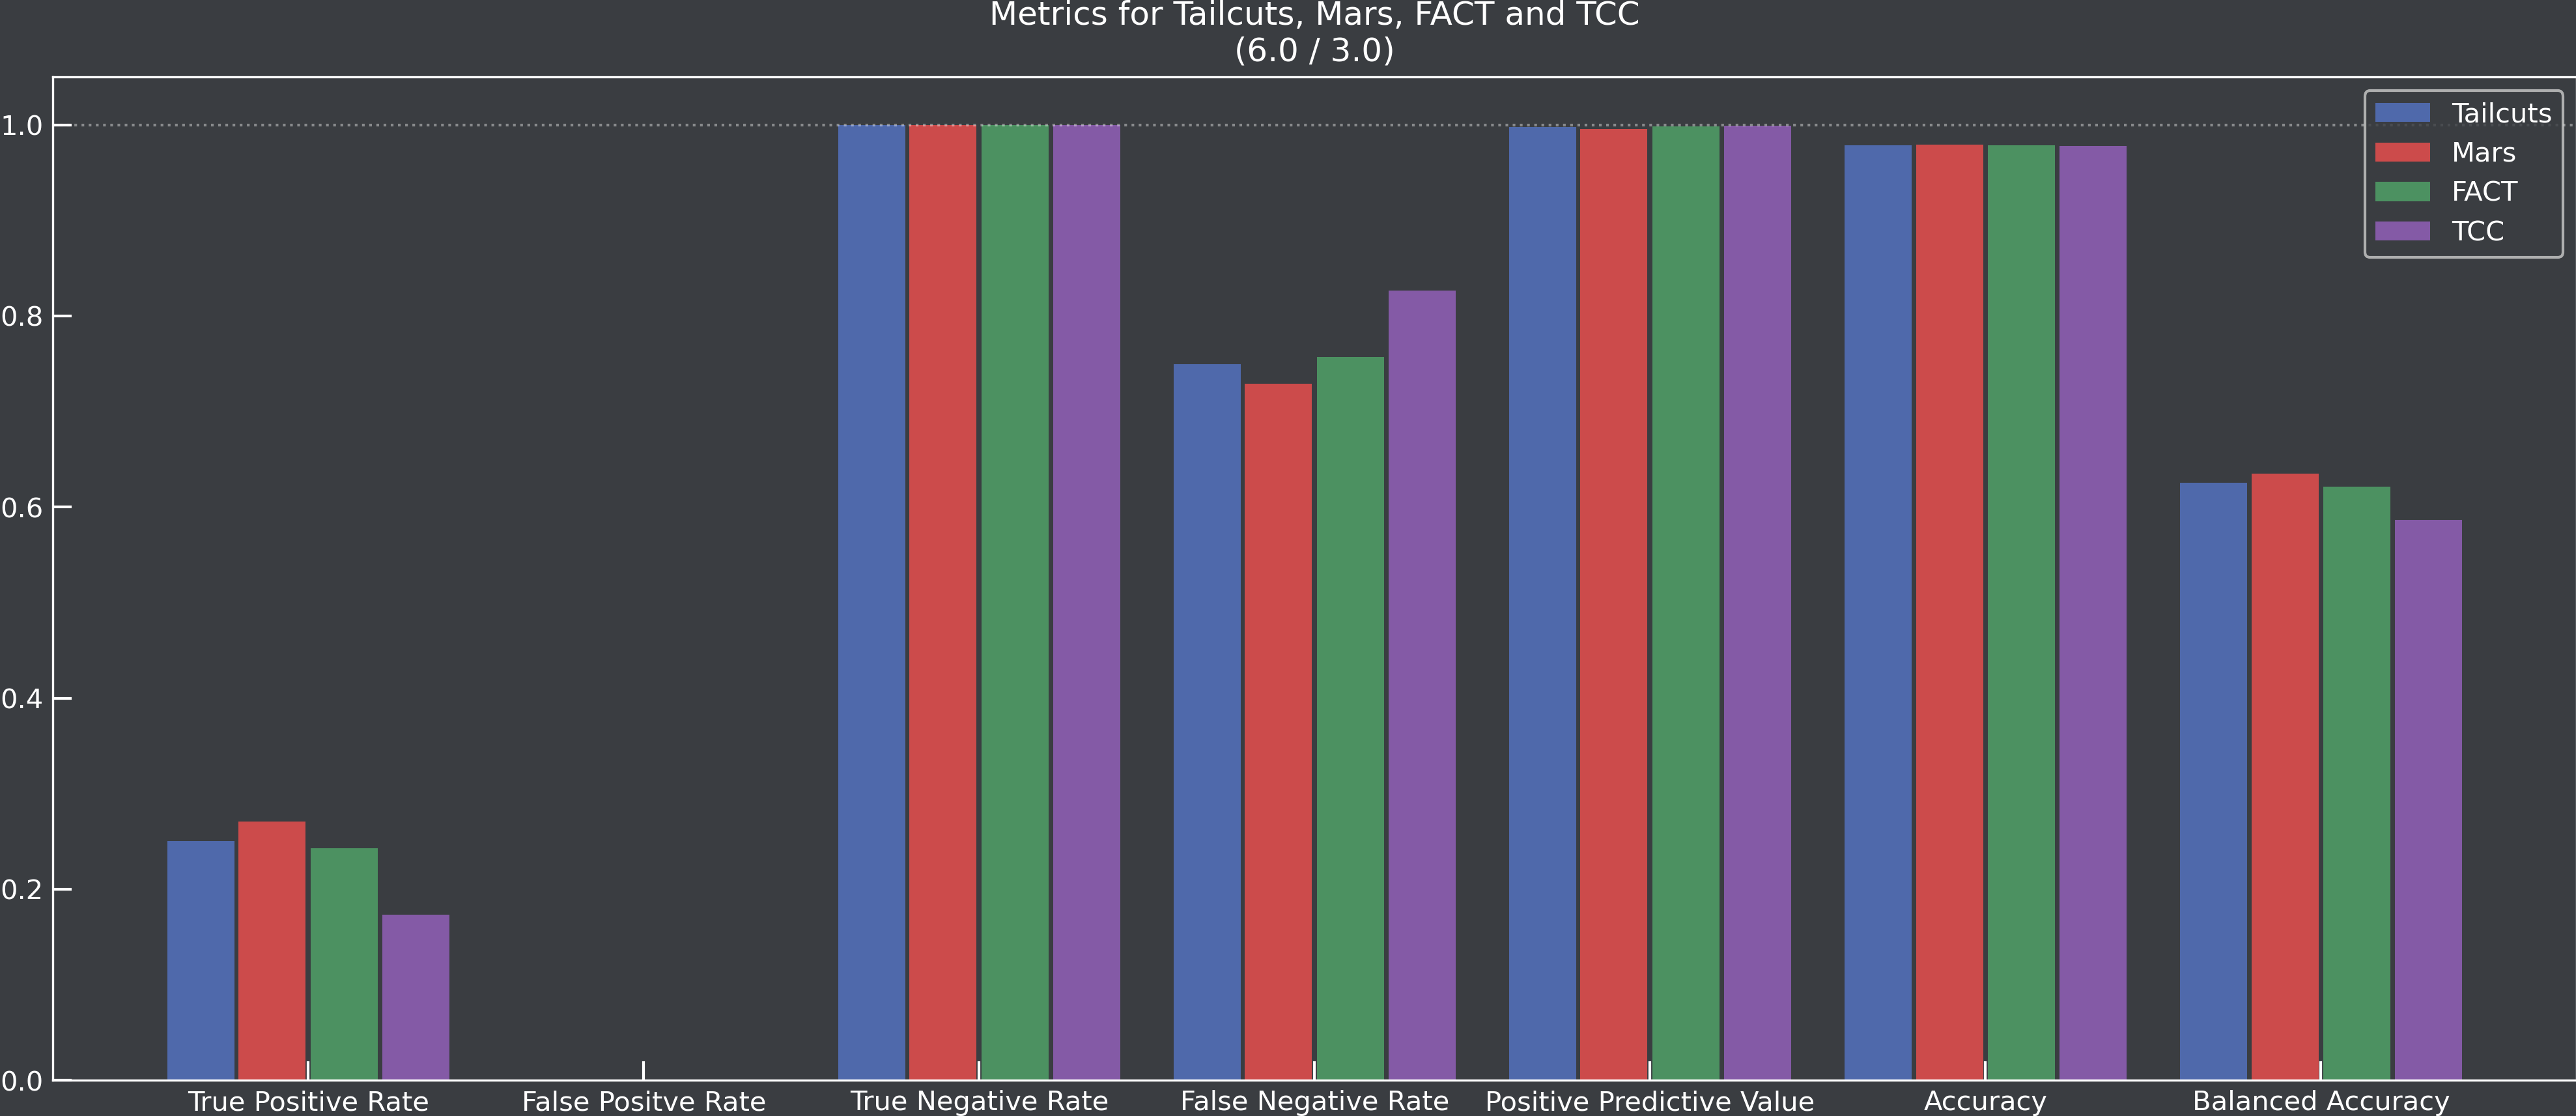
\includegraphics[width=\textwidth]{plots/metrics/metrics_6.0_3.0_dark.png}
    \else
      \centering
      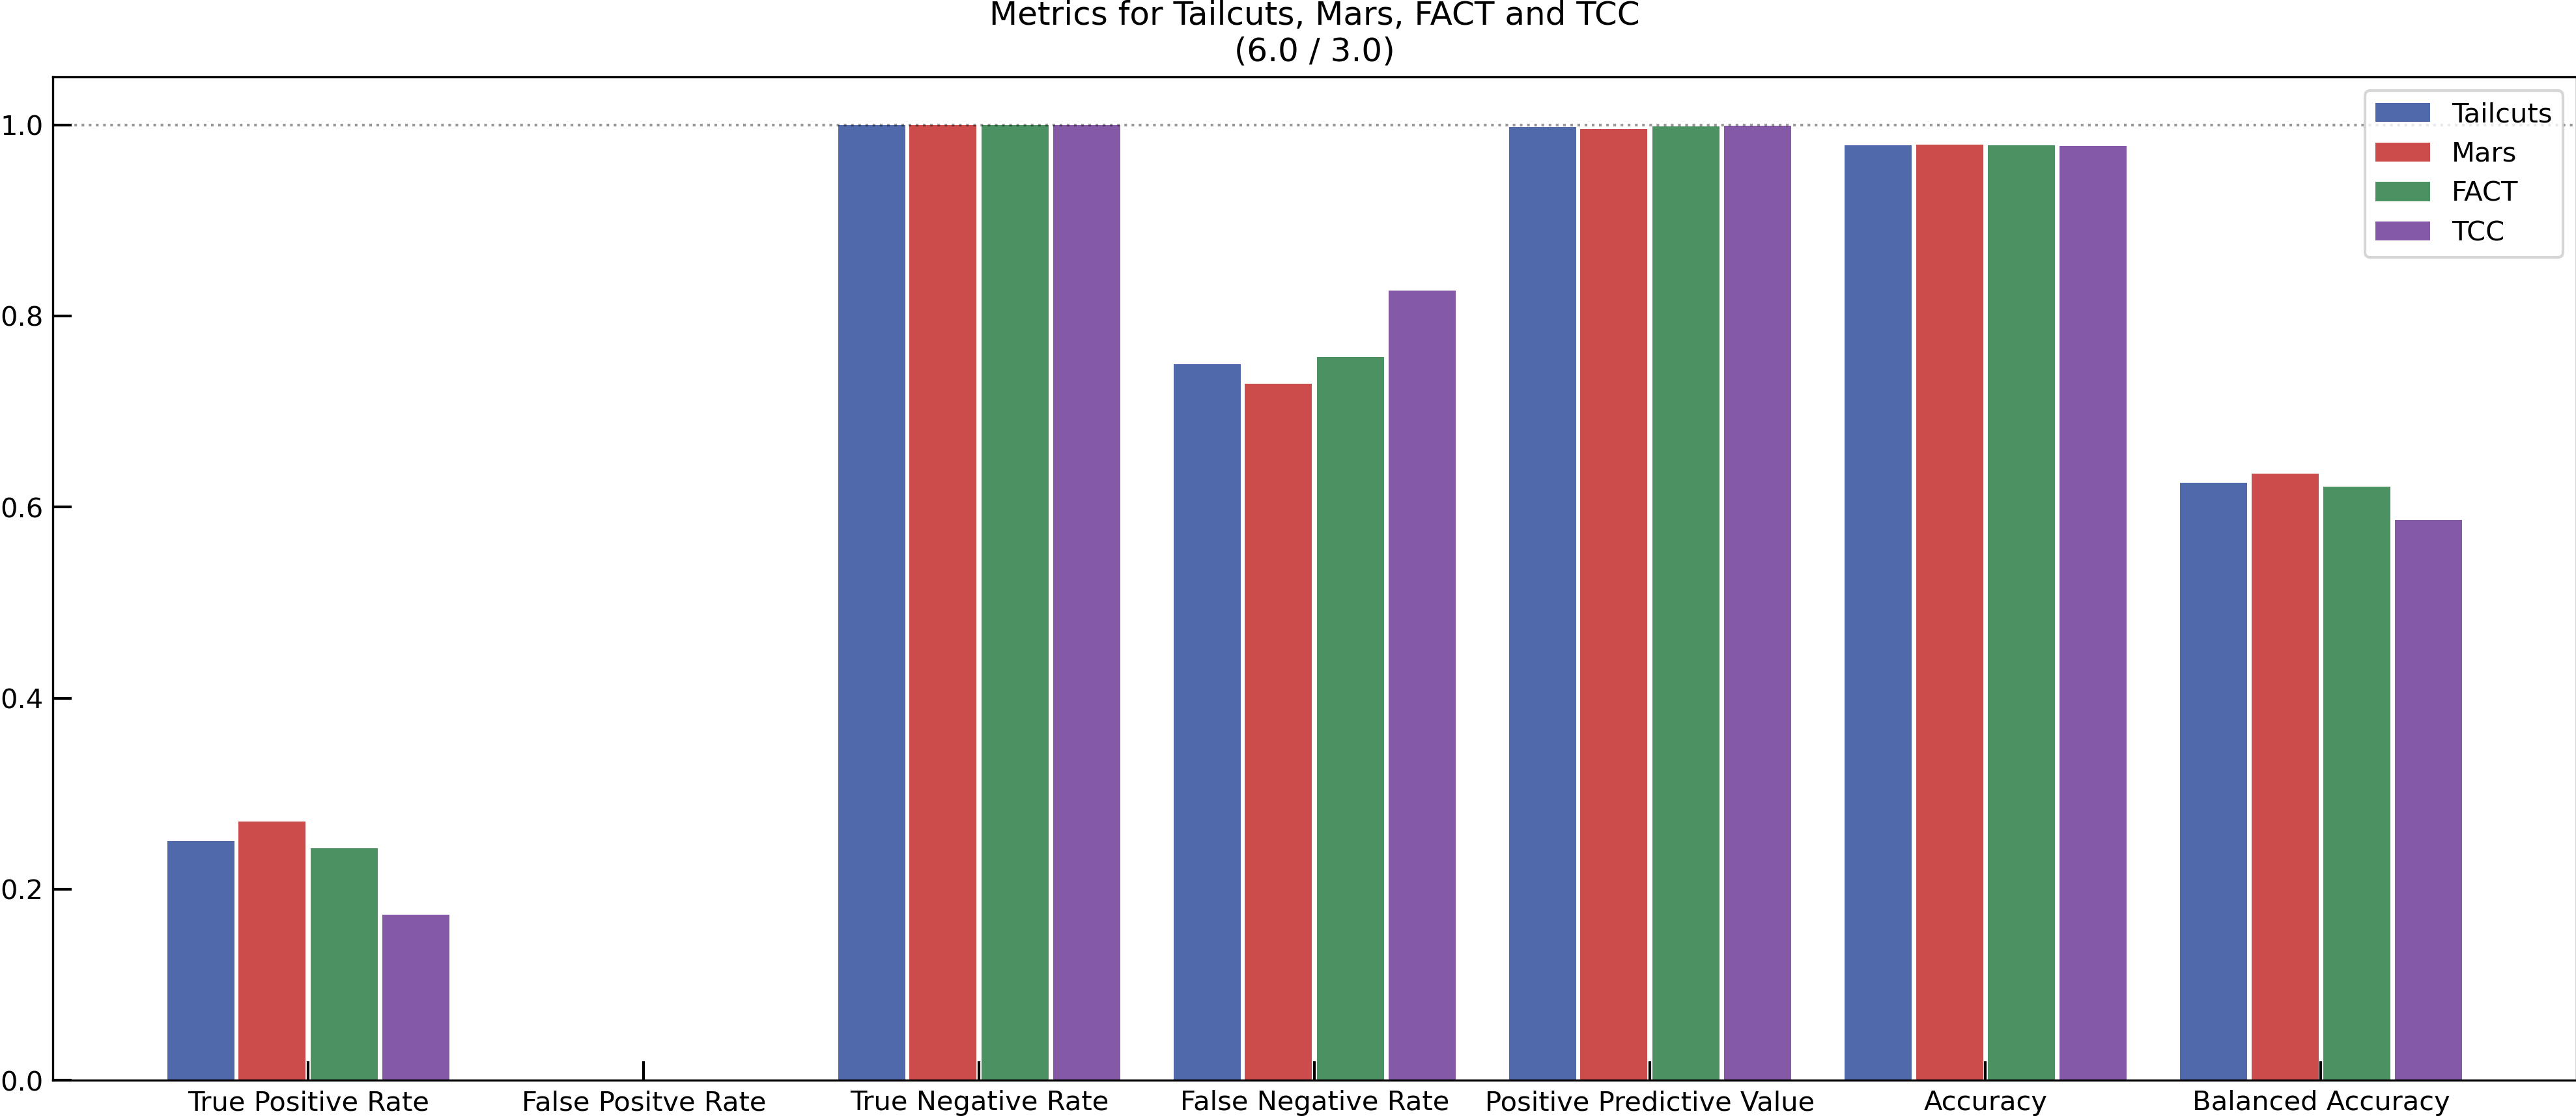
\includegraphics[width=\textwidth]{plots/metrics/metrics_6.0_3.0_light.png}
    \fi
  }
  \only<3>{
    \ifdefined\darktheme
      \centering
      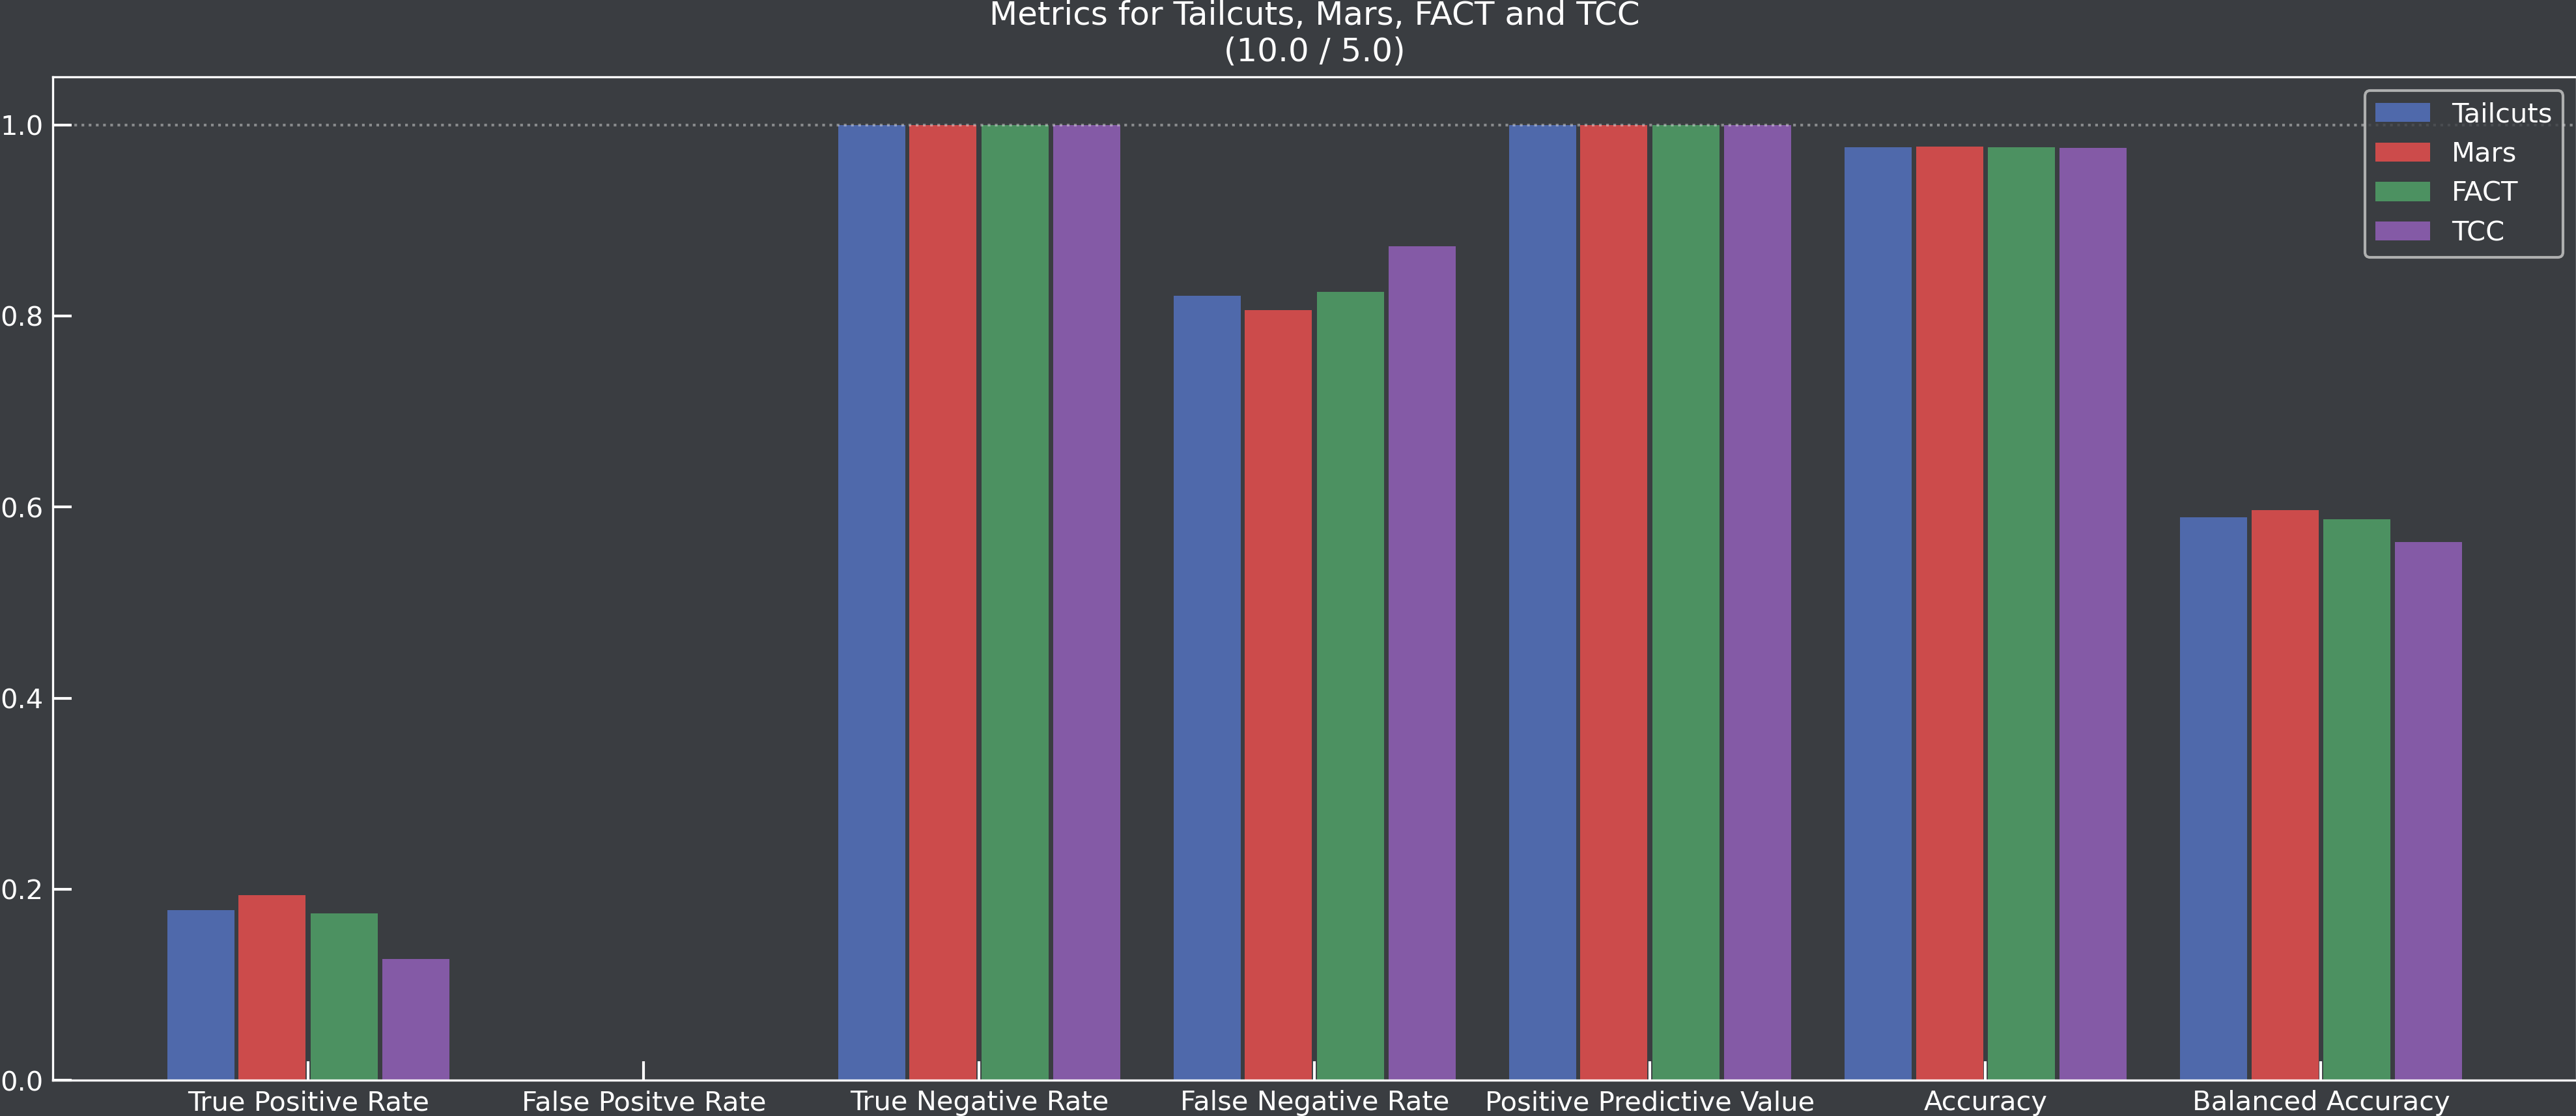
\includegraphics[width=\textwidth]{plots/metrics/metrics_10.0_5.0_dark.png}
    \else
      \centering
      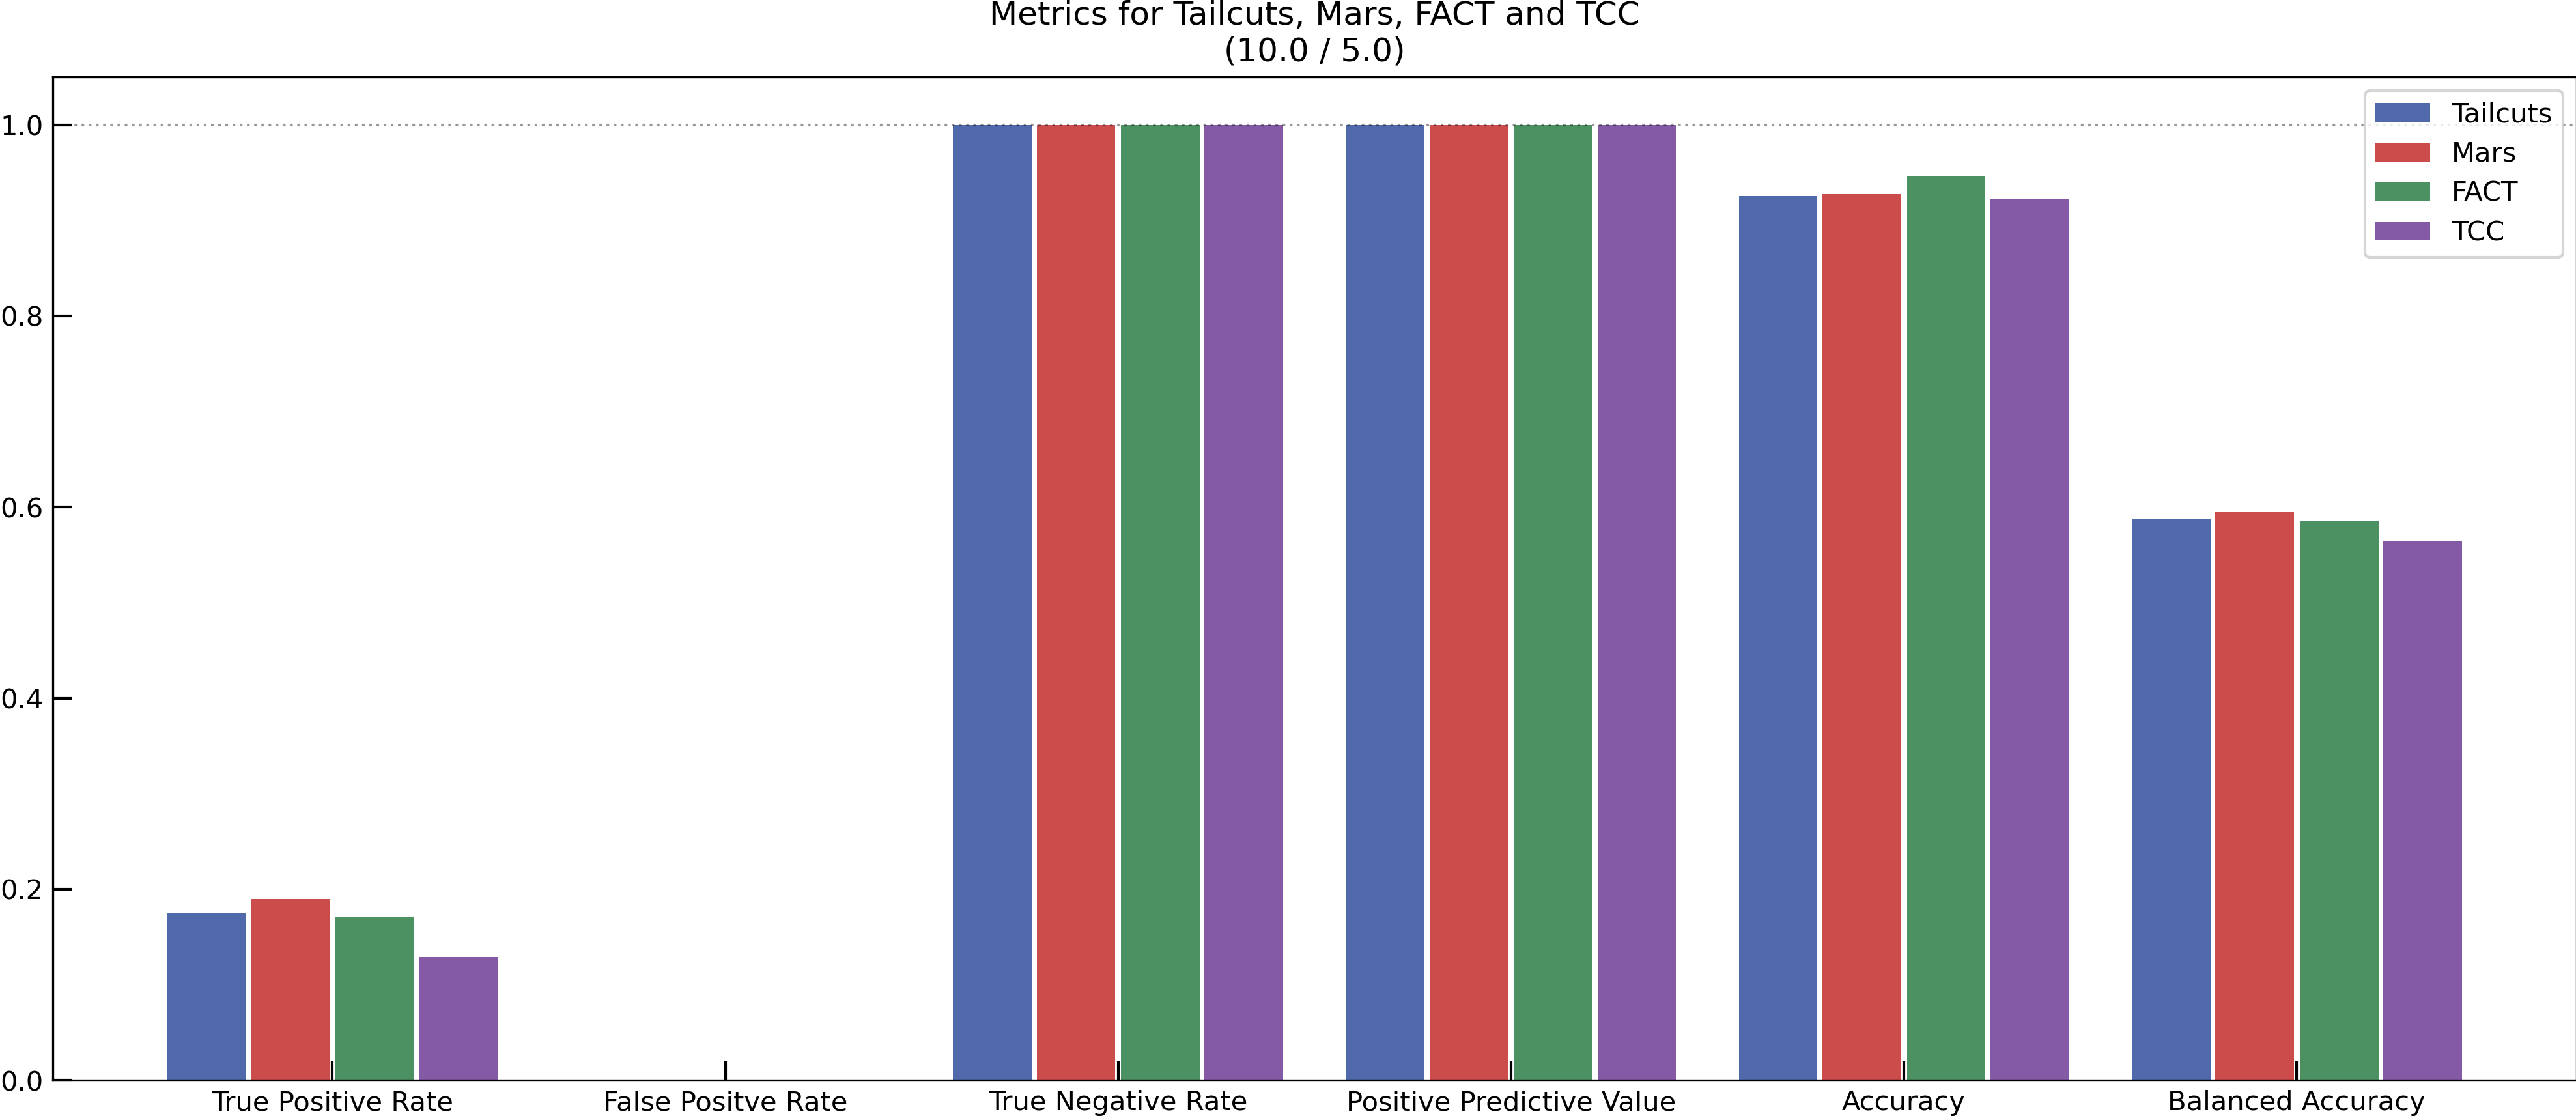
\includegraphics[width=\textwidth]{plots/metrics/metrics_10.0_5.0_light.png}
    \fi
  }
\end{frame}



\section{Outlook and Summary}
\begin{frame}
  \begin{center}
    \textbf{\huge Outlook and Summary}\\
    \begin{tikzpicture}
      \ifdefined\darktheme
        \draw [color=white] (0,0) -- (6,0);
        \draw [color=tugreen] (0,0) -- (6,0);
      \else
        \draw [color=darkgray] (0,0) -- (6,0);
        \draw [color=tugreen] (0,0) -- (6,0);
      \fi
    \end{tikzpicture}
  \end{center}
\end{frame}

\begin{frame}{Outlook}
    \begin{minipage}{0.7\textwidth}
        \begin{itemize}
            \ifdefined\darktheme
                \item Compare cleaners for other parameters than the \code{white!70!black}{picture} and \code{white!70!black}{boundary thresholds}
            \else
                \item Compare cleaners for other parameters than the \code{lightgray}{picture} and \code{lightgray}{boundary thresholds}
            \fi
            \begin{itemize}
                \ifdefined\darktheme
                    \item [\rightarrow] Use \code{white!70!black}{sklearn.model_selection.Parametergrid} to find the best parameters for each cleaner
                \else
                    \item [\rightarrow] Use \code{lightgray}{sklearn.model_selection.Parametergrid} to find the best parameters for each cleaner
                \fi
            \end{itemize}
            \ifdefined\darktheme
                \item Instead of letting the \code{white!70!black}{picture threshold} vary from \(\num{0}\) to \(\num{10}\), use quantiles
                \item Vary the \code{white!70!black}{boundary thresholds} as \(\num{0.25}\), \(\num{0.33}\), \(\num{0.5}\) and \(\num{0.75}\) of the \code{white!70!black}{picture threshold}
            \else
                \item Instead of letting the \code{lightgray}{picture threshold} vary from \(\num{0}\) to \(\num{10}\), use quantiles
                \item Vary the \code{lightgray}{boundary thresholds} as \(\num{0.25}\), \(\num{0.33}\), \(\num{0.5}\) and \(\num{0.75}\) of the \code{lightgray}{picture threshold}
            \fi
        \end{itemize}
    \end{minipage}
    \begin{minipage}{0.28\textwidth}
        
\includegraphics[width=\textwidth]{logos/sklearn.png}
    \end{minipage}
\end{frame}

\begin{frame}{Problems}
    \begin{itemize}
        \item Run time and number of datasets increase with the number of parameters
        \begin{itemize}
            \ifdefined\darktheme
                \item [\rightarrow] For \code{white!70!black}{TailcutsImageCleaner} and \code{white!70!black}{MarsImageCleaner} alone, this results in \(\num{32}\) possible combinations of parameters:
            \else
                \item [\rightarrow] For \code{lightgray}{TailcutsImageCleaner} and \code{lightgray}{MarsImageCleaner} alone, this results in \(\num{32}\) possible combinations of parameters:
            \fi
            \begin{center}
                \begin{tabular}{l}
                    \code{yamlblue}{params} \texttt{=} \textcolor{yamlyellow}{\{}\\
                    \qquad\code{yamlorange}{"picture_quantiles"}\texttt{:} \code{yamlyellow}{(}\texttt{0.9, 0.99, 0.995, 0.999}\code{yamlyellow}{)}\texttt{,}\\
                    \qquad\code{yamlorange}{"boundary_threshold_ratio"}\texttt{:} \code{yamlyellow}{(}\texttt{0.25, 0.33, 0.5, 0.75}\code{yamlyellow}{)}\texttt{,}\\
                    \qquad\code{yamlorange}{"min_number_picture_neighbors"}\texttt{:} \code{yamlyellow}{(}\texttt{1, 2}\code{yamlyellow}{)}\\
                    \qquad\textcolor{yamlyellow}{\}}
                \end{tabular}
            \end{center}
            \ifdefined\darktheme
                \item [\rightarrow] Add only two parameters for \code{white!70!black}{FACTImageCleaner} and this number increases to 64 possible combinations
            \else
                \item [\rightarrow] Add only two parameters for \code{lightgray}{FACTImageCleaner} and this number increases to 64 possible combinations
            \fi
            \begin{center}
                \begin{tabular}{l}
                    \code{yamlblue}{fact_params}\code{yamlyellow}{[}\code{yamlorange}{"time_limit"}\code{yamlyellow}{]} \texttt{=} \code{yamlyellow}{(}\texttt{2, 5}\code{yamlyellow}{)}
                \end{tabular}
            \end{center}
        \end{itemize}
    \end{itemize}
\end{frame}

\begin{frame}{Summary}
    \begin{minipage}[T]{0.48\textwidth}
    \begin{itemize}
        \setlength\itemsep{1em}
        \ifdefined\darktheme
            \item So far, a \code{white!70!black}{picture threshold} of \(\approx\num{6.0}\) seems to be the best choice w.r.t. the metrics
        \else
            \item So far, a \code{lightgray}{picture threshold} of \(\approx\num{6.0}\) seems to be the best choice w.r.t. the metrics
        \fi
        \begin{itemize}
            \item [\rightarrow] Has to be tested again for combinations with other parameters
        \end{itemize}
        \ifdefined\darktheme
            \item Testing other ratios than \(\num{0.5}\) for the \code{white!70!black}{boundary thresholds} seems to be a rational next step
            \item With \code{white!70!black}{sklearn}s \code{white!70!black}{ParameterGrid}, it is hopefully possible to find the best parameters for each cleaner
        \else
            \item Testing other ratios than \(\num{0.5}\) for the \code{lightgray}{boundary thresholds} seems to be a rational next step
            \item More combinations of parameters should help finding the optimal parameters for each cleaner
        \fi
    \end{itemize}
    \end{minipage}
    \begin{minipage}{0.48\textwidth}
        \begin{tikzpicture}
        \ifdefined\darktheme
            \roundpic[xshift=0cm,yshift=0, fill=darkmode]{7.8cm}{8cm}{plots/metrics_double_dark.pdf}{5}{2.3}
            \roundpic[xshift=-.1cm,yshift=-.2cm, fill=darkmode]{3.8cm}{3cm}{plots/simple_roc_dark.png}{0}{3.5}
            \roundpic[xshift=0cm,yshift=0, fill=darkmode]{3cm}{2.5cm}{plots/ang_res/ang_res_6.0_3.0_dark.png}{2}{1}
        \else
            \roundpic[xshift=0cm,yshift=0, fill=white]{7.8cm}{8cm}{plots/metrics_double_light.pdf}{5}{2.3}
            \roundpic[xshift=-.1cm,yshift=-.2cm, fill=white]{3.8cm}{3cm}{plots/simple_roc_light.png}{0}{3.5}
            \roundpic[xshift=0cm,yshift=0, fill=white]{3cm}{2.5cm}{plots/ang_res/ang_res_6.0_3.0_light.png}{2}{1}
        \fi
        \end{tikzpicture}
    \end{minipage}
\end{frame}

\end{document}
